%%%%%%%%%%%%%%%%%%%%%%%%%%%%%%%%%%%%%%%%
% Classe do documento
%%%%%%%%%%%%%%%%%%%%%%%%%%%%%%%%%%%%%%%%

% Nós usamos a classe "unb-cic".  Deixe apenas uma das linhas
% abaixo não-comentada, dependendo se você for do bacharelado ou
% da licenciatura.

%\documentclass[bacharelado]{unb-cic}
\documentclass[licenciatura]{unb-cic}



%%%%%%%%%%%%%%%%%%%%%%%%%%%%%%%%%%%%%%%%
% Pacotes importados
%%%%%%%%%%%%%%%%%%%%%%%%%%%%%%%%%%%%%%%%

\usepackage[brazil,american]{babel}
\usepackage[T1]{fontenc}
\usepackage{indentfirst}
\usepackage[square, numbers]{natbib}
\usepackage{xcolor,graphicx,url}
\usepackage[utf8]{inputenc}
\usepackage{array}
\graphicspath{{/image}}
\usepackage{dcolumn}
\usepackage{multirow}
\usepackage{longtable}
\newcolumntype{C}[1]{>{\centering\let\newline\\\arraybackslash\hspace{0pt}}m{#1}}




%%%%%%%%%%%%%%%%%%%%%%%%%%%%%%%%%%%%%%%%
% Cores dos links
%%%%%%%%%%%%%%%%%%%%%%%%%%%%%%%%%%%%%%%%

% Veja o arquivos cores.tex se quiser ver que outras cores estão
% pré-definidas.  Utilizando o comando \hypersetup abaixo nós
% evitamos aquelas caixas vermelhas feias em volta dos links.

%%%%%%%%%%%%%%%%%%%%%%%%%%%%%%%%%%%%%%%%
% Cores do estilo Tango
%%%%%%%%%%%%%%%%%%%%%%%%%%%%%%%%%%%%%%%%

\definecolor{LightButter}{rgb}{0.98,0.91,0.31}
\definecolor{LightOrange}{rgb}{0.98,0.68,0.24}
\definecolor{LightChocolate}{rgb}{0.91,0.72,0.43}
\definecolor{LightChameleon}{rgb}{0.54,0.88,0.20}
\definecolor{LightSkyBlue}{rgb}{0.45,0.62,0.81}
\definecolor{LightPlum}{rgb}{0.68,0.50,0.66}
\definecolor{LightScarletRed}{rgb}{0.93,0.16,0.16}
\definecolor{Butter}{rgb}{0.93,0.86,0.25}
\definecolor{Orange}{rgb}{0.96,0.47,0.00}
\definecolor{Chocolate}{rgb}{0.75,0.49,0.07}
\definecolor{Chameleon}{rgb}{0.45,0.82,0.09}
\definecolor{SkyBlue}{rgb}{0.20,0.39,0.64}
\definecolor{Plum}{rgb}{0.46,0.31,0.48}
\definecolor{ScarletRed}{rgb}{0.80,0.00,0.00}
\definecolor{DarkButter}{rgb}{0.77,0.62,0.00}
\definecolor{DarkOrange}{rgb}{0.80,0.36,0.00}
\definecolor{DarkChocolate}{rgb}{0.56,0.35,0.01}
\definecolor{DarkChameleon}{rgb}{0.30,0.60,0.02}
\definecolor{DarkSkyBlue}{rgb}{0.12,0.29,0.53}
\definecolor{DarkPlum}{rgb}{0.36,0.21,0.40}
\definecolor{DarkScarletRed}{rgb}{0.64,0.00,0.00}
\definecolor{Aluminium1}{rgb}{0.93,0.93,0.92}
\definecolor{Aluminium2}{rgb}{0.82,0.84,0.81}
\definecolor{Aluminium3}{rgb}{0.73,0.74,0.71}
\definecolor{Aluminium4}{rgb}{0.53,0.54,0.52}
\definecolor{Aluminium5}{rgb}{0.33,0.34,0.32}
\definecolor{Aluminium6}{rgb}{0.18,0.20,0.21}

\hypersetup{
  colorlinks=true,
  linkcolor=DarkScarletRed,
  citecolor=DarkScarletRed,
  filecolor=DarkScarletRed,
  urlcolor= DarkScarletRed
}



%%%%%%%%%%%%%%%%%%%%%%%%%%%%%%%%%%%%%%%%
% Informações sobre a monografia
%%%%%%%%%%%%%%%%%%%%%%%%%%%%%%%%%%%%%%%%

% definições prévias do documento
\title{Mineração de Dados Aplicada ao Estudo da Evasão e Desempenho dos Alunos do Bacharelado em Ciência da Computação da Universidade de Brasília}

\orientador{\prof \dr Jan Mendonça Correa}{CIC/UnB}
\coorientador[a]{\prof \drª Maria Emília Machado Telles Walter}{CIC/UnB}

\coordenador{\prof \dr Wilson Henrique Veneziano}{CIC/UnB}

\diamesano{26}{agosto}{2015}

                           
\membrobanca{\prof \drª Maria Emília Machado Telles Walter}{CIC/UnB}

\membrobanca{\drª Maria Inez Machado Telles Walter}{DPO/UnB}

\autor{Luiza Alencar}{Azevedo}
\coautor{Yago da Silva}{Santos}


\CDU{004.4}

\palavraschave{Evasão, Mineração de Dados, Informação, Análise Estatística, Ciência da Computação, Universidade de Brasília}
\keywords{Evasion, Data Mining, Information, Statistics Analysis, Computer Science, University of Brasilia}


%%%%%%%%%%%%%%%%%%%%%%%%%%%%%%%%%%%%%%%%
% Texto
%%%%%%%%%%%%%%%%%%%%%%%%%%%%%%%%%%%%%%%%

\begin{document}
  \maketitle
  \pretextual

  \begin{dedicatoria}
  	  	\begin{center}
  		"À minha família, que sempre esteve comigo me apoiando."
  		
  	- Luiza Alencar Azevedo
  	\end{center}
  	
  		\begin{center}
  			"À minha irmã Gilvânia \textit{(em memória)}, que foi e sempre será essencial em minha vida, minha história e em meu coração."
  			
  			- Yago da Silva Santos
  		\end{center}
  	
  \end{dedicatoria}

  \begin{agradecimentos}
   	
   	\begin{center}
   		"Agradeço à Deus por tudo que Ele proporcionou, agradeço também aos meus lindos pais Luiz Carlos e Júlia Alencar que sempre tiveram paciência, dedicação e amor em todos os momentos de minha vida. Agradeço à minha querida e maravilhosa irmã Marina Alencar que me deu suporte não somente durante minha graduação, mas sim durante meus vinte e três anos e também ao meu cunhado Leon Sólon. Agradeço imensamente ao meu atual noivo e futuro marido Vinícius Ramos que ajudou em todos os momentos difíceis e comemorou vitórias ao meu lado. 
   		\newline
   		Agradeço à todos meus colegas de graduação, em especial meu amigo Yago Santos que esteve comigo desde o início da graduação e que realizou esse trabalho ao meu lado, Guilherme Resende, José Fonseca, Érico Vinícius, Jéssica Naiara e Luísa Behrens que estiveram por perto durante toda essa jornada. Agradeço também aos meus amigos externos à UnB, que entenderam os momentos de ausência.
   		\newline
   		Agradeço aos professores que me apoiaram e principalmente aos meus queridos orientadores Jan Mendonça Correa e Maria Emilia Machado Telles Walter que não mediram esforços para nos ajudar."
   		
   		- Luiza Alencar Azevedo
   	\end{center}
   	
   	\begin{center}
   		"Agradeço primeiramente a Deus, pelo dom da vida e da fé. Aos meus familiares e amigos, em especial aos meus pais, José e Catarina, ao meu irmão Gilvan e minha cunhada Sheila, por todo o apoio e incentivo prestado desde o meu ingresso na Universidade, por entenderem as minhas ausências, por estarem sempre ao meu lado e acreditarem em mim. A minha irmã Gilvânia (em memória), que enquanto em vida sempre me acompanhou nos estudos e se preocupou com o meu futuro. A minha madrinha Juciléia, pelo constante apoio nos momentos mais difíceis.  Aos meus colegas de curso, pela convivência diária, pelos momentos de descontração e ajuda ao decorrer da graduação. A minha colega de trabalho e amiga Luiza Alencar e ao Vinícius Ramos, que me acompanharam desde o ínicio do curso e divertiram as tardes de estudo (sem contar os cafés tomados juntos). Aos professores do Departamento de Ciência da Computação, em especial aos orientadores Jan Mendonça Correa e Maria Emília Machado Telles Walter, por todo suporte prestado durante o desenvolvimento deste trabalho, pelas ideias, sugestões e dedicação em nos ajudar. "
   		
   		- Yago da Silva Santos
   	\end{center}
   	
  \end{agradecimentos}

\selectlanguage{brazil}  
\begin{resumo}
 A evasão no ensino superior é um problema que aflige as Instituições de Ensino públicas e privadas. A aprovação do aluno em uma Instituição de Ensino Superior não é suficiente para garantir que o mesmo permaneça e conclua a graduação. Analisando estudos anteriores realizados no Departamento de Ciência da Computação da Universidade de Brasília, verificou-se que as taxas de reprovação nas disciplinas obrigatórias iniciais são altas e que as taxas de evasão estão em crescimento. Por meio do processo de mineração de dados e análise estatística, esse trabalho visa obter informações que permitam ao Departamento identificar as principais causas de evasão nos semestres iniciais no Bacharelado em Ciência da Computação.
  \end{resumo}

  \selectlanguage{american}
  \begin{abstract}
  The evasion in higher education is a problem that afflicts the institutions of public and private education. The approval of the student in a higher education institution is not enough to ensure that it remains complete and graduation. Analyzing previous studies in the Department of Computer Science at the University of Brasilia, it was found that repetition rates in the early compulsory subjects are high and the dropout rates are on the rise. Through data mining and statistical analysis process, this work aims to obtain information to enable the Department to identify the main causes of dropout in the early semesters Bachelor of Computer Science.
  \end{abstract}
  \selectlanguage{brazil}

  \tableofcontents
  \listoffigures
  \listoftables

  \textual
  \textual

\chapter{Introdução} \label{1title1}
	
Todo ser humano tem o direito a educação, que deve ser garantida pelo Estado. Na verdade, é a própria Constituição de 1988 \citep{constituicao} que a enuncia como direito de todos, dever do Estado e da família, com as funções de garantir a realização plena do ser humano, inseri-lo no contexto do Estado Democrático e qualificá-lo para o mundo do trabalho. A um só tempo, a educação representa tanto mecanismo de desenvolvimento pessoal do indivíduo, como da própria sociedade em que ele se insere~\citep{raposo2005}.

A educação é mais que uma simples aquisição de saber. Ela propicia o desenvolvimento e a participação política ativa. É imprescindível para o desenvolvimento político e econômico, para a democracia e para a igualdade social, trazendo sustentabilidade para uma sociedade que deseja evoluir.

\section{Evasão no Ensino}

Um grande problema enfrentado pelas Instituições de Ensino fundamental e médio, e também de nível superior, é a saída dos estudantes sem conclusão dos estudos. A admissão não assegura a inclusão efetiva desses estudantes e tampouco sua permanência, sendo necessárias medidas mais eficazes que garantam a finalização escolar e acadêmica.

A evasão no ensino é um fenômeno social complexo, definido como interrupção no ciclo de estudos~\citep{gaioso2005} e tornou-se um problema que vem preocupando as Instituições de Ensino em geral, sejam elas públicas ou particulares, pois a saída de alunos provoca graves consequências sociais, acadêmicas e econômicas~\citep{baggi_lopes2010}. A perda com a evasão dos alunos pode ser mensurável em termos quantitativos, mas em termos qualitativos, torna-se uma tarefa com maior grau de complexidade. Isso porque a saída do aluno, sem a consequente conclusão de seu curso, traz perdas implícitas. Para ~\citet[p. 1]{lobo2011}, a evasão representa \textit{“uma perda social, de recursos e de tempo de todos os envolvidos no processo de ensino, pois perdeu o aluno, seus professores, a instituição de ensino, o sistema de educação e toda a sociedade (ou seja, o País)”}.

A evasão é um problema que aflige as Instituições de Ensino em geral. Conforme o Resumo Técnico do Censo da Educação Superior de 2009, desenvolvido pelo Ministério da Educação em parceria com Instituto Nacional de Pesquisas Anísio Teixeira (MEC/INEP) \citep{censo_2009}, os índices no âmbito universitário são altos e vêm sendo uma realidade cada vez mais presente nas Instituições de Ensino Superior. Em 2007, o Plano Nacional de Educação (PNE) fixou o objetivo de diminuir a taxa de evasão de alunos do ensino superior \citep{dias2010}.

Segundo ~\citet{braga2003}, o estudo e a análise sobre a evasão no ensino superior brasileiro apresenta-se  como uma proposta relevante, mas em contrapartida há poucas pesquisas disponíveis, visto que os estudos desenvolvidos a respeito de evasão escolar no Brasil iniciaram-se a partir de 1980. Para os autores, a evasão pode ser resultada por dois aspectos diferentes, seja pela própria iniciativa do aluno em sair do sistema de ensino ou pela conjuntura de fatores escolares, econômicos e pessoais, em que os dois primeiros aspectos podem corroborar mais para uma exclusão do que para uma evasão propriamente dita. Essa é uma questão atual, que está em pauta e que se agrava cada vez mais, conforme veremos adiante neste trabalho. E a construção de um modelo que permita identificar as causas e reduzir os índices de evasão no ensino superior brasileiro ainda é uma incógnita.

Em algumas análises divulgadas sobre o ingresso e evasão no Ensino Superior no Brasil, é notório o baixo percentual de alunos formados nos cursos pertencentes à área de Exatas \citep{censo2013}, tais como Ciências, Matemática e cursos ligados à área de Computação (tais como Ciência da Computação, Sistemas de Informação, Processamento de Dados e Automação). No levantamento  realizado pelo Sindicato das Entidades Mantenedoras de Estabelecimentos de Ensino Superior no Estado de São Paulo (Semesp), divulgado pelo portal  \citet{portalg1}, foi apontado que nos cursos de Sistemas de Informação, a cada três estudantes ingressantes, um chega a concluir os estudos. No caso da Ciência da Computação, a cada quatro ingressantes, apenas um conclui o curso, o que representa uma taxa de evasão de 75\%. O estudo divulgado pela Associação Brasileira das Empresas de Tecnologia da Informação e Comunicação ~\citep{brasscom} apontou que em 2010 o índice de evasão nos cursos de Tecnologia da Informação no Brasil foi de 87\%. No mesmo estudo, foi projetado que até o ano de 2014 poderia haver um \textit{déficit} de 45 mil profissionais para a área, e até 2022 seriam necessários 900 mil novos profissionais. Um segundo estudo realizado pela Associação Brasileira das Empresas de Tecnologia da Informação e Comunicação (Brasscom) sobre matrículas e concluintes para os cursos relacionados à TIC em Instituições de Ensino Superior ~\citep{brasscom2} (levando em consideração o triênio 2007-2009), apontou que no Distrito Federal, o número de concluintes dos cursos relacionados à TIC representam apenas 12,5\% sobre os matriculados, tendo sido registrados 7.779 matriculados e apenas 970 concluintes.

Sob essa perspectiva, alguns estudos foram realizados no Departamento de Ciência da Computação da Universidade de Brasília (CIC-UnB), com o objetivo de avaliar dados e informações que possibilitariam caracterizar as informações gerais sobre os cursos ofertados, as disciplinas e o público atendido pelo Departamento, o que envolveu a análise das taxas de ingresso, reprovação e evasão dos alunos matriculados. Atualmente, o Departamento de Ciência da Computação é responsável pela oferta de disciplinas em quatro cursos superiores: Bacharelado em Ciência da Computação, Licenciatura em Computação, Bacharelado em Engenharia da Computação  e Bacharelado em Engenharia Mecatrônica. Destes estudos, foi detalhado que a taxa de evasão dos alunos do Bacharelado em Ciência da Computação era de 55,76\% \citep{palmeira_santos2014}, o que pode ser considerado um número preocupante, assim como a diferença de matrícula e formandos por gênero, em que os alunos do sexo masculino representavam a maior proporção do público atendido pelo curso.

\section{Justificativa} \label{1title4}

Tendo em vista a alta taxa de evasão dos cursos ofertados pelo Departamento de Ciência da Computação da Universidade de Brasília, principalmente para o Bacharelado em Ciência da Computação, torna-se necessário um estudo que permita avaliar os motivos que podem levar o aluno à evasão, e estabelecer critérios que permitam identificar quais alunos têm maior propensão a evadir do curso logo nos semestres iniciais. Esse estudo pode contribuir para que o Departamento, em conjunto com os coordenadores e docentes, possam estabelecer medidas a fim de evitar que esse percentual aumente ao longo dos semestres consecutivos, e assim possibilitar a formação de um número maior de alunos para a área de Computação na Universidade de Brasília.

Nos últimos anos, a evasão no Bacharelado em Ciência da Computação na Universidade de Brasília está sendo utilizada como objeto de estudo de alunos e professores, que buscam identificar fatores que possam acarretar a desistência do aluno, e que auxiliem na identificação de alunos que estejam ou venham a estar sob risco de evasão.
Em trabalhos anteriores, foram identificados que os quatro primeiros semestres do curso são os que apresentam maiores taxas de evasão. Partindo desse pressuposto, surge a proposta de aprofundar o estudo de causas ou variáveis que possam estar relacionadas ao processo de evasão nos períodos iniciais, e formular uma análise que permita identificar novos padrões nos dados do departamento e predizer qual perfil de aluno tem maior propensão a evadir do curso.

\section{Problema} \label{1title6}

Atualmente, não há variáveis ou informações que permitam identificar alunos em risco de evasão no Bacharelado em Ciência da Computação da Universidade de Brasília.

\section{Objetivos} \label{1title2}

O objetivo geral deste trabalho é analisar e identificar as variáveis e fatores que justifiquem ou que estejam relacionadas a evasão nos primeiros semestres do curso de Ciência da Computação da Universidade de Brasília.


Os objetivos específicos constituem em:
\begin{itemize}
	\item Selecionar e organizar os dados fornecidos para análise;
	\item Realizar experimentos com dados oficiais do Bacharelado em Ciência da Computação;
	\item Identificar variáveis e padrões que possam estar relacionados com o processo de evasão no Bacharelado em Ciência da Computação da Universidade de Brasília;
	\item Discutir os resultados obtidos.     
\end{itemize}


\section{Hipótese} \label{1title3}
É possível identificar, por meio da mineração de dados, padrões nas causas de evasão dos alunos nos primeiros semestres do Bacharelado em Ciência da Computação da Universidade de Brasília.


\section{Descrição dos Capítulos} \label{1title5}

O Capítulo \ref{2title} aborda a evasão no Ensino Superior, destacando as causas e implicações na gestão das Instituições de Ensino Superior, além de apresentar trabalhos relacionados à evasão nos cursos de Computação realizados no Brasil, incluindo análises no Departamento de Ciência da Computação da Universidade de Brasília.

O Capítulo \ref{chapter4} aborda os conceitos de dado, informação e conhecimento, e a importância dos sistemas de informação e a gestão do conhecimento para as organizações. O Capítulo \ref{chapter3} apresenta o conceito, os componentes e as técnicas de mineração de dados, além das etapas do processo de extração do conhecimento, conhecido como KDD. É apresentado o \textit{software} Weka, utilizado na etapa de mineração de dados e algumas das funcionalidades disponíveis. 

O Capítulo \ref{chapter5} descreve a metodologia adotada para a análise e mineração dos dados, baseado nas etapas do processo KDD. Os resultados obtidos da análise estatística e mineração de dados são apresentados no Capítulo \ref{chapter6}, e o Capítulo \ref{chapter7} apresenta as conclusões obtidas e sugestões para trabalhos futuros.





	


  \chapter{A Evasão nas Instituições de Ensino Superior} \label{2title}

A evasão nas Instituições de Ensino Superior é um problema antigo, mas pouco explorado no meio educacional. Os cursos de Ciências Exatas, tais como Matemática, Física e Ciência da Computação, geralmente apresentam taxas de alunos formados inferiores se comparadas às outras áreas de conhecimento \citep{censo2013}. Neste capítulo, será abordado o conceito, fatores e situações que justifiquem as taxas de evasão na área de Computação, objeto de estudo desta pesquisa. A Seção \ref{2title1} retrata o panorama da Educação Superior conforme o Censo da Educação Superior de 2013. A Seção \ref{2title2} aborda os conceitos de evasão, exclusão e mobilidade, além das implicações que a evasão acarreta ao aluno e ao sistema de ensino. A Seção \ref{2title3} aponta os principais motivos apontados para justificar a evasão dos alunos dos cursos de graduação, incluindo análises de evasão no âmbito da Universidade de Brasília. A Seção \ref{2title4} apresenta estudos relacionados à evasão nos cursos de Computação no Brasil. A Seção \ref{2title5} apresenta estudos realizados sobre evasão nos cursos de Computação da Universidade de Brasília, e a Seção \ref{2title6} apresenta a análise dos resultados observados nas  Seções \ref{2title4} e \ref{2title5}. 

\section{O Cenário da Educação Superior no Brasil} \label{2title1}

Anualmente, o Censo da Educação Superior, realizado pelo Instituto Nacional de Estudos e Pesquisas Educacionais Anísio Teixeira (INEP)~\footnote{\url{http://portal.inep.gov.br}}, vinculado ao Ministério da Educação~\footnote{\url{http://www.mec.gov.br}} fornece dados que permitem analisar a Educação Superior no Brasil. O Censo Escolar consiste na levantamento e análise de dados estatísticos educacionais do cenário nacional.

De acordo com os resultados obtidos pelo Censo da Educação Superior de 2013 \citep{censo_site}, no Brasil haviam 32.049 cursos de graduação, sendo 30.791 presenciais e 1.258 a distância. Também foram contabilizadas 2.391 Instituições de Ensino Superior, sendo 301 públicas e 2.090 particulares, conforme mostrado na Tabela \ref{instituiçoes}. As Instituições particulares correspondem a 87,41\% das Instituições de Ensino Superior no Brasil, e deste total, 89,76\% correspondem à faculdades privadas.

\begin{table}[!h]
	\caption{Número de Instituições de Ensino Superior no Brasil em 2013.} 	\label{instituiçoes}
	\centering
	\begin{tabular}{C{4cm}|C{3cm}C{3cm}}
		\hline
		Categoria & \multicolumn{2}{c}{Quantidade}\\
		\hline
		& Pública & Privada\\ \hline
		Universidade & 111 & 84\\
		Centro Universitário & 10 & 130\\
		Faculdade & 140 & 1.876\\
		IF e Cefet~\footnote{IF: Institutos Federais; Cefet: Centro Federal de Educação Tecnológica.} & 40 & -\\
		\hline
	\end{tabular}
\end{table}

Em 2013, foram registrados 7,3 milhões de alunos matriculados no ensino superior, representando um crescimento de 3,8\% em relação ao ano de 2012. Entre o ano de 2012 e 2013, foi verificado um crescimento de 4,5\% na rede privada e 1,9\% na rede \citep{censo2013}. Em 2013, as universidades atendiam 53,4\% e as faculdades 29,2\% das matrículas. Em relação ao ano de 2003, foi verificado um crescimento de 76,4\% no número de matrículas, conforme apresentado na Figura \ref{graficoCenso}. 

\begin{figure}[!h]
	\centering
	{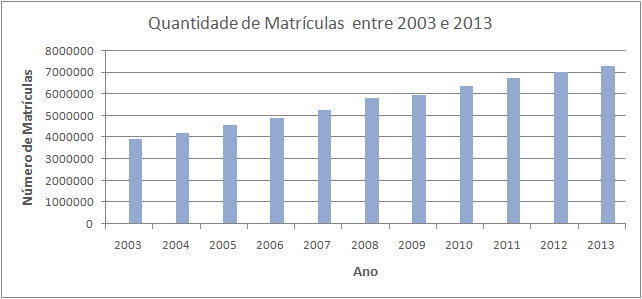
\includegraphics[width=13cm, height=6cm]{images/censo_matriculas}}
	\caption {Quantidade de matrículas registradas pelo Censo da Educação Superior entre o ano de 2003 e 2013.}
	\label{graficoCenso}
\end{figure}

A Figura \ref{distribuicao} apresenta a distribuição das matrículas por tipo de Instituição de Ensino Superior. As universidades eram responsáveis por 70,8\%, os centros universitários por 25,2\%, as faculdades por 3,2\%, e os institutos federais e centros federais de educação tecnológica por 0,8\% das matrículas efetivas em 2013. As Instituições privadas eram responsáveis por 86,6\% e as Instituições públicas 13,4\% das matrículas.

\begin{figure}[!h]
	\centering
	{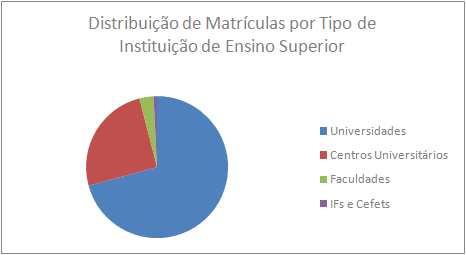
\includegraphics[width=12cm, height=6cm]{images/distribuicao}}
	\caption {Distribuição de Matrículas por tipo de Instituição de Ensino Superior. As universidades eram responsáveis pelo maior percentual de matrículas efetivas em 2013.}
	\label{distribuicao}
\end{figure}

Dos 1.951.354 alunos ingressantes em 2013, 56,44\% são do sexo feminino e 45,34\% do sexo masculino. Das 6.152.405 matrículas registradas, 55,52\% são do sexo feminino e 44,48\% do sexo masculino. Dos 829.938 alunos concluintes, 59,24\% são do sexo feminino e 40,76\% do sexo masculino. Analisando o quantitativo de matrículas efetivas, alunos formados e concluintes por tipo de Instituição, as Instituições de Ensino Superior privadas são responsáveis por atender uma maior demanda de alunos, conforme apresentado na Tabela \ref{atendimento}. Outro dado revelado pelo Censo é que as Instituições de Ensino Superior públicas abrangem aproximadamente 28,9\% das matrículas efetivas, e as Instituições de Ensino Superior privadas aproximadamente 71,1\%.

\begin{table}[!h]
	\caption{Número de alunos atendidos pelas Instituições de Ensino Superior públicas e privadas.} 	\label{atendimento}
	\centering
	\begin{tabular}{C{4cm}|C{3cm}C{3cm}}
		\hline
		Categoria & \multicolumn{2}{c}{Quantidade}\\
		\hline
		& Pública & Privada\\ \hline
		Alunos Ingressantes & 456.864 & 1.494.490\\
		Matrículas Efetivas & 1.777.974 & 4.374.431\\
		Alunos Concluintes & 206.261 & 623.677\\ \hline
	\end{tabular}
\end{table}

A Tabela \ref{areas} mostra o percentual de matrículas, ingressantes e concluintes por área geral de curso. A área de Ciências Sociais, Negócios e Direito apresentou o maior percentual de matrículas, ingressantes e concluintes em 2013, seguida da área de Educação. Nas áreas de Engenharia, Produção e Construção, Ciência, Matemática e Computação, e Agricultura e Veterinária, o percentual de concluintes é menor se comparado ao percentual de matriculados e ingressos.

\begin{table}[!h]
	\caption{Percentual de Matrículas, Ingressantes e Concluintes por Área de Atuação em 2013.} 	\label{areas}
	\centering
	\begin{tabular}{C{7cm}|C{2cm}C{2,5cm}C{2,5cm}}
		\hline
		Área de Atuação & \multicolumn{3}{c}{Percentual (\%)}\\
		\hline
		& Matrículas & Ingressantes & Concluintes \\ \hline
		Ciências Sociais, Negócios e Direito & 40,6 & 41,5 & 44,3\\
		Educação & 18,8 & 17,2 & 20,3\\
		Saúde e Bem Estar Social & 13,5 & 12,5 & 14,1\\
		Engenharia, Produção e Construção & 14 & 14,8 & 8,2\\
		Ciência, Matemática e Computação & 6,1 & 6,5 & 5,6\\
		Agricultura e Veterinária & 2,4 & 2,1 & 1,9\\
		Humanidades e Artes & 2,2 & 2,4 & 2,7\\
		Serviços & 2,3 & 3,1 & 2,9\\
		\hline
	\end{tabular}
\end{table}

 
Em contraste ao crescimento do número de ingressantes, os resultados também apontaram uma redução na quantidade de alunos formados nas Instituições de Ensino Superior brasileiras. Em 2013, foram contabilizados 991.010 alunos formandos nos cursos de graduação em todo o Brasil, 5,7\% a menos em relação ao ano de 2012, que contabilizou 1.050.413 alunos formandos \citep{censo2012}. Analisando a taxa de concluintes por tipo de Instituição de Ensino Superior, foi verificada uma redução aproximada de 6,7\% nas Instituições privadas e de 3,5\% nas Instituições públicas em relação ao ano de 2012. 

Apesar do crescimento e expansão do acesso ao Ensino Superior nos últimos anos no Brasil, percebe-se ainda que o número de concluintes é inferior ao número de matrículas efetivas. Tomando como exemplo a área de Ciências, Matemática e Computação, apenas 12,5\% dos alunos foram identificados como concluintes em 2013, se comparado ao total matrículas efetivas para a área no mesmo período. Conforme destacado por \citet{tigrinho2008}, apenas o ingresso do aluno nos cursos de graduação não é suficiente para garantir a permanência e conclusão do ensino superior. 

A fim de identificar e compreender as causas de desistência ou abandono escolar nos cursos de graduação, estudos e pesquisas a respeito da evasão escolar vêm crescendo e ganhando destaque no meio educacional. \citet{lobo2011} e \citet{dias2010} destacam a evasão como uma dos principais problemas em qualquer nível de ensino, que aflige as Instituições de Ensino em geral, sejam elas públicas ou particulares.
 

\section{O Conceito de Evasão e sua Implicação na Gestão das Instituições de Ensino Superior} \label{2title2}

A evasão escolar tem se tornado um  objeto de estudo nos diferentes níveis da educação, desde a educação básica até o ensino superior. Embora no Brasil o número de pesquisas relacionadas ao assunto tenha crescido nos últimos anos, \citet{lobo2011} afirma que ainda não existem estudos suficientes que abordem a evasão no cenário nacional, sendo a maioria das análises limitadas a casos isolados (limitados a uma Instituição de Ensino Superior ou a um docente), se comparados aos países desenvolvidos. No sentido geral, a evasão escolar pode ser caracterizada pelo abandono ou interrupção dos estudos, de forma voluntária ou involuntária, que pode ser influenciado por uma conjunção de fatores internos ou externos ao indivíduo. \citet{gaioso2005} interpreta a evasão escolar como a interrupção dos estudos, sem a sua conclusão. 

O conceito de evasão, por sua vez, pode ser confundido com o conceito de exclusão e mobilidade. Para \citet[p. 13]{bueno1993}, a evasão é caracterizada pelo desligamento voluntário do aluno, por sua própria vontade e responsabilidade, enquanto que a exclusão \textit{"implica na admissão de uma responsabilidade da escola e de tudo que a cerca por não ter mecanismos de aproveitamento e direcionamento do adolescente que se apresenta para uma formação profissionalizante."} Do mesmo modo, \citet{ristoff1997} traz o paralelo entre os conceitos de evasão e mobilidade, onde a evasão corresponde ao abandono dos estudos, enquanto a mobilidade caracteriza-se pela mudança de curso, como uma tentativa de se encontrar êxito ou felicidade sobre suas reais possibilidades e potencialidades.

A evasão pode estar relacionada a fatores institucionais, pessoais e externos. E pode consistir em evasão de um curso, de uma universidade ou do sistema de ensino superior. Nesse sentido, a Comissão Especial de Estudos sobre Evasão \citep{mec_1997} define o processo de evasão em três níveis: evasão do curso, evasão da instituição e evasão do sistema.

A evasão do curso é aquela que o aluno deixa o curso por alguma razão, podendo permanecer na mesma Universidade, ou mudar para outro curso de outra Instituição de Ensino Superior ou abandonar os estudos universitários. De acordo com o \citet{mec_1997}, esse tipo de evasão pode ocorrer por abandono, mudança de curso, desistência ou exclusão por norma institucional. Em qualquer dos casos, o aluno é desligado do curso, o que consiste em uma evasão, e essa deverá ser estudada para que outras perdas de mesma natureza sejam evitadas. A evasão da instituição é aquela que ocorre quando um estudante vai para uma outra Instituição de Ensino Superior, o que ocorre na maior parte das vezes por um problema de gestão e de insatisfação do estudante com o ambiente educacional. E existe também a evasão do sistema, onde o aluno interrompe o ensino superior, seja temporariamente ou definitivamente. Esse tipo de evasão é que demanda mais atenção por parte do Governo, pois pode implicar em mudanças na políticas públicas de educação, desde questões institucionais, acadêmicas ou até mesmo individuais. A evasão escolar não é problema restrito somente ao Brasil. Segundo \citet{silvafilho2007}, a evasão no ensino superior é uma problemática internacional, que exerce impacto nos resultados sobre os sistemas educacionais. 

Um apontamento interessante  destacado por \citet{silvafilho2007} é a ausência de programas que visem a permanência do aluno junto à instituição de ensino. Nas instituições privadas, um grande esforço de propaganda e \textit{marketing} é empregado para atrair novos alunos, porém tal esforço não é destinado à manutenção dos alunos já matriculados. Para \citet[p. 642]{silvafilho2007}, \textit{"as perdas de estudantes que iniciam mas não terminam seus cursos são desperdícios sociais, acadêmicos e econômicos"}, o que acarreta na perda de recursos e receitas, pois tornam-se investimentos sem retorno, sejam estes financeiros ou não. Segundo o pesquisador Oscar Hipólito, do Instituto Lobo para o Desenvolvimento da Educação, da Ciência e da Tecnologia~\footnote{Publicação disponível em \url{http://g1.globo.com/educacao/noticia/2011/02/pais-perde-r-9-bilhoes-com-evasao-no-ensino-superior-diz-pesquisador.html}}, as perdas financeiras com evasão no ensino superior em 2009 alcançou a marca de 9 bilhões de reais.

\citet{tigrinho2008} também caracteriza as perdas ocorridas no processo de evasão escolar. Para o autor, há perdas de caráter econômico, tanto para o aluno quanto para a Instituição de Ensino. As instituições podem ser afetadas pela perda de prestígio e impactos financeiros, principalmente as Instituições de Ensino Superior privadas. \citet{lobo2011} também salienta os possíveis prejuízos para as Instituições de Ensino Superior privadas. Uma vez que os cursos são planejados tomando por base a quantidade de alunos pagantes, a geração de vagas ociosas pode acarretar em problemas gerenciais e afetar a viabilidade dos cursos e das próprias Instituições, visto que a redução das receitas podem comprometer os planos administrativo-financeiro e acadêmico.

\citet{braga2003} demonstram que, ao estudar a evasão, outros aspectos relacionados à Instituições de Ensino Superior também devem ser considerados, tais como a avaliação da estruturas curriculares dos cursos, participação dos docentes e discentes na elaboração das propostas curriculares, metodologias pedagógicas empregadas, cultura organizacional do ambiente escolar e a figura do docente em sala de aula. Conforme \citet{baggi_lopes2010}, uma análise abrangente do âmbito da instituição é capaz de revelar informações que podem ser úteis para a resolução de problemáticas enfrentadas, na revisão de processos utilizados e no aprimoramento do ensino. Portanto, a evasão não deve ser atribuída somente ao aluno, passando a ser também uma reflexão sobre a própria estrutura geral da Instituição, o que envolve um processo de análise qualitativa e quantitativa como um todo. \citet[p. 59]{favero2013}  \textit{apud} \citet{lobo2011} salientam que a questão da evasão deve ser trabalhada em conjunto com todos os membros da Instituição de Ensino Superior, num esforço coletivo entre os profissionais da área acadêmica e administrativo-financeira, de modo que as ações desenvolvidas de combate à evasão não sejam vistas \textit{"apenas como uma gestão de marketing ou atendimento, mas fazer parte das ações estratégicas, com planejamento, execução, acompanhamento e avaliação".} Conforme o \citet[p. 19]{mec_1997}, 
\begin{quotation}
\textit{"Compreender a evasão como um processo implica superar a postura economicista, derivada de visão essencialmente utilitarista da formação universitária que, se levada a extremos, conduziria, por exemplo, à extinção de alguns cursos que são hoje mantidos quase que exclusivamente pelas universidades públicas. Logo, os índices de diplomação, retenção e evasão devem ser examinados em conjunto, não como um fim em si mesmos, ou apenas com objetivos "rankeadores", mas sim como dados que possam contribuir tanto à identificação dos problemas a eles relacionados, como à adoção de medidas pedagógicas e institucionais capazes de solucioná-los".}
\end{quotation}

\section{Motivos para Evasão} \label{2title3}

A evasão é um problema complexo, que pode ser resultante de uma conjunção de vários fatores que pesam na decisão do aluno de permanecer ou não no curso \cite{tigrinho2008}. As causas para a desistência são variadas, mas o essencial é que o aluno não pare de estudar por falta de condições. Alguns fatores são citados como os mais recorrentes:

\begin{itemize} 
\item \textit{Repetência:} O baixo rendimento e a reprovação em disciplinas consideradas difíceis influenciam na decisão de continuar ou não os estudos, principalmente se esta ocorre nos semestres iniciais. Essa é considerada a causa principal de evasão. Um fator que também pode contribuir para repetência, conforme destaca \citet{tigrinho2008}, é a forma de avaliação utilizada pela Instituição de Ensino;

\item\textit{ Baixa eficiência durante o Ensino Médio:} Esse item relaciona-se diretamente com a repetência, pois o aluno que passa na seleção do vestibular mas não possui uma base de conhecimento consolidada provavelmente encontrará dificuldades de adaptação e não conseguirá realizar um bom acompanhamento durante o curso;

\item \textit{Falta de conhecimento acerca dos cursos e escolha precoce da especialidade funcional:} São mais de 150 opções de cursos superiores e, a cada dia, surgem novas opções de carreiras e de oportunidades de trabalho. A escolha da profissão geralmente acontece muito cedo, geralmente logo após o término do Ensino Médio. A indecisão é normal nessa fase e muitas vezes não se investiga as opções de cursos pelos melhores critérios. A escolha pode advir de uma expectativa irreal que é frustrada após a entrada do estudante na Universidade. A falta de informações sobre a profissão e o curso em que os alunos ingressam leva muitos à evasão. Ao perceberem que agiram movidos por ideias infundadas a respeito da instituição ou da profissão escolhida, se decepcionam com o curso superior e a Instituição de Ensino. Logo passam a considerar a possibilidade de desistência;

\item \textit{Mudança de curso:} Há vários fatores que podem levar o estudante a mudar de curso, como a não identificação com o curso atual, dificuldades nas disciplinas, mudança de área em que se deseja atuar, entre outros. A mudança pode ocorrer tanto na mesma Instituição de Ensino (no caso ocorre somente a mudança de curso), como para outras Instituições de Ensino Superior (neste caso, pode ser que o aluno queira continuar no mesmo curso, mas em outra Instituição). Em muitos casos, há a possibilidade de aproveitamento de disciplinas equivalentes, o que facilita tal mobilidade entre cursos;

\item \textit{Desprestígio da profissão:} Conforme destacado por Tigrinho (2008), esse fator está muitas vezes está relacionado à visão que foi e é construída sobre o curso e a área de atuação. Áreas como Medicina, Engenharia e Direito, por exemplo, pressupõem para muitas pessoas prestígio social, salários acima da média e maiores e facilitadas chances de empregabilidade. Por outro lado, percebe-se o oposto em cursos como as Licenciaturas, marcadas por sobrecarga na jornada de trabalho e salários reduzidos se comparados à outras áreas de atuação, o que contribui para que a falta de prestígio e visibilidade da profissão diante do mercado de trabalho;

\item \textit{Restrições nos financiamentos estudantis e dificuldades financeiras:} Mesmo com a existência e expansão de programas que visem contribuir com os custos de um curso superior, tais como o Fundo de Financiamento Estudantil (FIES) e o Programa Universidade para Todos (PROUNI), ainda não é suficiente para atender todos os alunos que não possuem meios financeiros para se manter na Universidade;

\item \textit{Horário do trabalho:} Muitas pessoas trabalham que têm a necessidade de trabalhar e estudar ao mesmo tempo podem encontrar dificuldades quanto à conciliação de horários. As pessoas, na maioria das vezes, trabalham durante o dia e estudam a noite, ou vice-versa. Quando ocorre esse conflito de horários, conforme destaca \citet{tigrinho2008}, os estudos tendem a ser deixados em segundo plano;

\item \textit{Desmotivação:} Motivação é um impulso que faz que as pessoas ajam e deem o melhor de si para atingir um determinado objetivo. Conforme destaca \citet{tigrinho2008} \textit{"ao ingressar na educação superior, o aluno é motivado, dentre outras razões, pela expectativa de melhores condições de vida e de realização profissional".} Porém, o autor ressalta que o fato de ser aprovado em um vestibular e realizar a matrícula em um curso superior não são fatores determinantes para a continuidade no curso ou na Instituição de Ensino Superior, tendo em vista que são motores diversos os que estimulam o estudante a continuar os estudos. A motivação é uma força intrínseca e descobrir formas de recriá-la sempre que necessário é a chave para que os estudantes não desistam;

\item \textit{Docentes despreparados para o ensino:} Muitas vezes o professor tem muito conhecimento, mas não tem o preparo para lidar com o aluno na sala de aula. Não possui didática para o ensino e pode estar desmotivado devido à pouca valorização da carreira, não se importando com o aluno de forma individual. E a cobrança de desempenho do professor por parte da Instituições de Ensino Superior e dos alunos é baixa;

\item \textit{Fatores externos:} Outros fatores que não estejam relacionados diretamente com a Instituição de Ensino Superior, mas ao próprio aluno, podem influenciar no processo de evasão. \citet{tigrinho2008} lista alguns fatores que são baseados na visão de alunos, tais como a falta de orientação e imaturidade na escolha do curso, busca por herança profissional (quando os filhos seguem a mesma profissão dos pais) e a falta da mesma (quando os pais conseguem ser bem-sucedidos sem possuir um curso superior), reprovações sucessivas devido à dificuldade de aprendizagem e assimilação dos conteúdos, assim como nascimento de filhos e casamentos não planejados, o que reflete na evasão, principalmente de mulheres que possuem piores condições financeiras. Há outros razões para desligamento com menor peso e que são imprevisíveis, como problemas de saúde (o que pode impedir o acesso do aluno à Instituição de Ensino Superior por algum tempo), falecimento e mudança de endereço dos alunos (o que pode dificultar a locomoção por meios de transporte até a Instituição de Ensino Superior).
\end{itemize}

Os fatores que podem levar o aluno à evasão são distribuídos em três categorias, a saber \citep{mec_1997}:

\begin{itemize}
	\item Fatores externos às Instituições;
	\item Fatores internos às Instituições;
	\item Fatores individuais dos estudantes.
\end{itemize}

Os fatores externos às Instituições de Ensino estão relacionados ao mercado de trabalho, reconhecimento da carreira escolhida, qualidade das instituições de ensino fundamental e médio, conjuntura econômica, inferiorização da profissão (exemplo das Licenciaturas), dificuldades financeiras do discente, adaptação ao ambiente da Instituição de Ensino Superior nos campos tecnológicos, econômicos e sociais e a ausência de políticas governamentais voltadas para a graduação. 

Os fatores internos as Instituições de Ensino estão relacionados com questões de caráter particular da própria Instituição de Ensino Superior, tais como questões acadêmicas  (como matrizes curriculares desatualizadas e falta de esclarecimentos sobre o Projeto Pedagógico de Curso - PPC), didático-pedagógicas (critérios adotados inadequadamente para realizar a avaliação do ensino), despreparo ou desinteresse do corpo docente, ausência de programas institucionais voltados ao estudante, cultura institucional que não valoriza a atividade docente e insuficiência na estrutura de apoio ao ensino de graduação.

Os fatores individuais dos estudantes estão ligados às características particulares do indivíduo, tais como personalidade, habilidade de estudo, formação acadêmica anterior, dificuldades de adaptação à vida universitária, escolha precoce do curso, incompatibilidades entre os campos de estudo e trabalho, desmotivação diante da opção de curso, dificuldades no processo de ensino-aprendizagem e mudanças de curso em decorrência de novos interesses. Nessa categoria, um ou mais fatores podem contribuir para o processo de evasão, e estão intimamente ligados ao sujeito, que podem ser influenciados de forma direta ou indireta pelo meio ao qual está inserido. Uma das causas apontadas por \citet{mec_1997} é a idade precoce onde se estabelece a escolha do curso e da profissão, além da falta de informações complementares sobre a carreira a ser escolhida. Geralmente, em torno dos 17 anos, o aluno se vê de certa forma obrigado a escolher qual carreira seguir. A mudança para o cenário do ensino superior também é um fator a ser considerado, o que requer transformações socioculturais de adaptação ao meio acadêmico e profissional. 

\subsection{Situações de Evasão na Universidade de Brasília} \label{2title31}

De acordo com a Secretaria de Administração Acadêmica da \citet{unb_saa}, a evasão (aqui mencionada como desligamento) no âmbito da Instituição de Ensino pode ser caracterizada pelas seguintes situações:
\begin{itemize}
	\item \textit{Desligamento por Abandono de Curso:} ocorre quando o aluno deixa de matricular-se em disciplinas ou quando registra 25\% ou mais de faltas nas disciplinas cursadas durante dois semestres letivos consecutivos;  
	\item \textit{Desligamento por Jubilamento:} ocorre quando o aluno ultrapassa o tempo máximo de permanência para conclusão do curso, conforme previsto pelo Conselho Nacional de Educação (CNE);
	\item \textit{Desligamento por Não-Cumprimento de Condição:} ocorre quando o aluno é identificado com risco de desligamento (seja por rendimento acadêmico ou por tempo de permanência no curso), e não tenha cumprido a condição que lhe foi imposta pelos órgãos colegiados;
	\item \textit{Desligamento Voluntário:} ocorre quando o aluno, por própria vontade, tenha desistido de manter seu vínculo com determinado curso na Universidade de Brasília, ou tenha sido aprovado por novo vestibular, obrigando o aluno a escolher entre o curso atual ou o novo curso; 
	\item \textit{Transferência para Outras Instituições de Ensino Superior:} ocorre quando o aluno, por meio de solicitação formal e declaração de reserva de vaga, tenha garantida sua vaga em outra IES por meio de transferência obrigatória ou facultativa, a fim de dar continuidade aos estudos.
	
\end{itemize}

O levantamento realizado em 2011 pela Diretoria de Acompanhamento e Integração Acadêmica (DAIA), setor vinculado ao Decanato de Ensino e Graduação (DEG) da Universidade de Brasília \citep{unb1}, apontou que a média de desligamentos dos alunos ingressantes entre o ano de 2002 e 2006 era de 34\%. O principal motivo apontado pela pesquisa foi o baixo rendimento dos alunos, onde foi verificada uma taxa de evasão de 44\% nos cursos da área de Exatas, e nos cursos de Licenciatura, onde em alguns cursos como Letras, História e Ciências Sociais, a evasão chega a superar 60\%. Seguido do baixo rendimento, outros motivos apontados para a evasão foi o abandono e desligamento voluntário, que representaram 41\% dos motivos apontados para a evasão. A Tabela \ref{evasao1} apresenta as taxas de evasão por motivos entre o ano de 2002 e 2006, conforme divulgação no portal da \citet{unb1}. 

\begin{table} [!h]
	\centering
	\caption{Percentual de evasão entre 2002 e 2006 na Universidade de Brasília \citep{unb1}.} 
	\begin{tabular}{C{5,5cm}|C{1,5cm}C{1,5cm}C{1,5cm}C{1,5cm}C{1,5cm}}
		\hline
		\multicolumn{1}{c}{Motivo} & \multicolumn{5}{|c}{Ano}\\ \hline
		& 2002 & 2003 & 2004 & 2005 & 2006\\
		\hline
		Baixo Rendimento & 38,2\% & 38,6\% & 35,1\% & 36,5\% & 34,5\%\\
		Abandono & 33,5\% & 29\% & 28,7\% & 28,7\% & 28,5\%\\
		Desligamento Voluntário & 16,8\% & 16,9\% & 18,9\% & 17,3\% & 16,9\%\\
		Outros & 11,4\% & 15,4\% & 17,3\% & 17,5\% & 20,1\%\\\hline
	\end{tabular}
	\label{evasao1}
\end{table}

Ao analisar as principais formas de ingresso na Universidade de Brasília (vestibular e Programa de Avaliação Seriada - PAS) entre 2002 e 2006, o estudo apontou que a taxa de evasão por baixo rendimento acadêmico é maior para os alunos que ingressaram pelo vestibular, em torno de 12\%, enquanto que pelo PAS a média é de 9\%. Em relação ao índice de formatura, foi verificado que dos alunos que ingressaram pelo vestibular em 2006, aproximadamente 39\% formaram-se nos cursos de graduação. Para os alunos ingressantes pelo PAS no mesmo período, esse percentual aumenta para 47\%.

Outro estudo divulgado pela \citet{unb2} em 2012 mostrou que entre o ano de 2002 e 2010, a taxa de evasão caiu de 42\% para 11\%. Mesmo com a diminuição do percentual de abandono, este valor ainda foi considerado alto de acordo com o Decanato de Ensino e Graduação (DEG) da Universidade de Brasília. Durante o período observado, obteve-se uma taxa média de evasão de 25\%. Entre o ano de 2009 e 2010, a taxa de evasão diminuiu de 27\% para 11\%. Dentre os motivos apontados para a evasão, foram verificados a demora no tempo para a conclusão da graduação, mudança de curso e falta de condições financeiras, fator este que contribui para o aumento das taxas de abandono dos cursos de graduação.

\section{Estudos sobre Evasão nos Cursos de Computação no Brasil} \label{2title4}

Alguns estudos foram realizados no Brasil por autores que buscaram investigar as causas e fatores que influenciam no processo de evasão dos cursos de Computação, com o objetivo de detalhar ou descobrir informações que possam justificar as crescentes taxas de evasão na área de Informática. 

O estudo desenvolvido por \citet{carniel2013} consistiu em identificar fatores que poderiam influenciar na evasão de alunos do curso de Ciência da Computação ofertado pela Universidade do Vale do Itajaí (UNIVALI), utilizando algoritmos e técnicas de mineração de dados em suas análises. Durante o processo, foram analisados dados dos alunos do período de 2008 a 2012, com o auxílio de banco de dados e da ferramenta Weka \citep{weka} (a ser detalhada no Capítulo \ref{chapter3})para o processo de mineração dos dados. Dos resultados obtidos pela pesquisa, foram constatados alguns aspectos:

\begin{itemize}
\item A diminuição do número de ingressantes durante o período analisado, assim como o aumento das taxas de evasão por abandono do curso;
\item As taxas de evasão tendem a ser maiores entre o  primeiro e terceiro períodos;
\item No semestre que evadem, a maioria dos alunos estão cursando disciplinas correspondentes às áreas de Matemática, Programação e Infraestrutura;
\item Algoritmos e Programação, Matemática Computacional, Álgebra Linear, Cálculo e Computação Básica são as disciplinas com maior frequência de alunos matriculados no período em que ocorre a evasão;
\item A faixa etária dos alunos com maior índice de evasão corresponde a 18 e 21 anos de idade;
\item 16\% dos alunos do total de evadidos obtiveram menções nas disciplinas acima de 8, e desta porcentagem, a maioria possui idade igual ou superior a 22 anos;
\item As notas obtidas nas disciplinas cursadas pelos alunos não mostraram influenciar de forma direta no processo de evasão.
\end{itemize}

O trabalho de \citet{prietch_pazeto2010} buscou investigar a evasão nos cursos de Licenciatura em Informática ofertados pela no \textit{campus} universitário de Rondonópolis, pertencente à Universidade Federal do Mato Grosso (UFMT). A análise foi realizada sobre dados dos alunos correspondentes entre 2001 (período em que o curso foi implantado) e 2009. Na pesquisa, foram empregadas técnicas de contato telefônico e via \textit{e-mail} com os alunos para a obtenção dos dados, assim como um levantamento sobre o índice de reprovação nas disciplinas que compõem a matriz curricular do curso. No estudo, fica evidente a dificuldade dos alunos em relação às disciplinas introdutórias do curso, tais como as que envolvem a aplicação de matemática e programação, que constituem os pilares para o conhecimento a ser adquirido no decorrer do curso. Da análise realizada, foram constatados os seguintes aspectos:

\begin{itemize}
\item As taxas de matriculados no curso são maiores no primeiro ano, e reduzem nos anos subsequentes;
\item As disciplinas com maior índice de reprovação no primeiro ano são as disciplinas de Cálculo 1, Álgebra para Computação, Programação I e Lógica Matemática, com média de reprovação em torno de 50,51\%;
\item As turmas são menores a partir do segundo ano de curso;
\item As disciplinas de Cálculo Numérico e Projeto e Análise de Algoritmos apresentam a maior taxa de reprovação dentre as matérias do terceiro ano;
\item A disciplina Projeto Final de Curso apresenta o maior grau de reprovação do último ano de curso;
\item Como justificativas para a dificuldade em disciplinas na área de Exatas, foram apontados aspectos como dificuldade em interpretação, métodos aplicados ao ensino pelo docente, divergências entre o que trabalhado em aula e o que é cobrado como avaliação, assim como a falta de articulação entre teoria e prática.
\end{itemize}

Outro estudo sobre evasão foi detalhado por \citet{rissi_marcondes2013}, realizado na Universidade Estadual de Londrina (UEL), tomando por base os dados relacionados à retenção (2010), reprovação (entre 2010 e 2012) e evasão (entre 2003 e 2012) dos cursos de graduação da Instituição de Ensino. No curso de Ciência da Computação, foi identificado em 2010 que a maior porcentagem de retenção\footnote{De acordo com a UEL, foram descritos os seguintes critérios para retenção de um aluno: \textit{"(i) reprovar por nota ou falta em mais de duas atividades acadêmicas; (ii) reprovar por nota e falta em mais de uma disciplina; e (iii) reprovar na disciplina essencial"}. \cite{rissi_marcondes2013}} encontra-se no terceiro e quarto ano do curso. 

Em relação a análise de reprovação entre 2010 e 2012, observou-se no primeiro ano de curso um maior grau de reprovação nas disciplinas de Matemática Discreta e Finita, Cálculo A  e Álgebra Linear. Já no segundo ano, as disciplinas com maior índice de reprovação foram Cálculo B  e Linguagens Formais e Autômatos. Nos anos seguintes, as taxas de reprovação em sua maioria eram superiores à 50\% para as disciplinas listadas acima. Em contrapartida, ao analisar os índices de evasão durante 2003 e 2012, percebeu-se uma diminuição entre o total de evadidos a partir de 2009 e um aumento na quantidade de alunos ativos, passando de 2,27\% em 2004 para 90\% em 2012. Na análise, os anos com maiores índices de evasão foram os de 2004, com uma taxa registrada de 50\% (22 evadidos entre 44 ingressantes) e de 2009, com uma taxa de 41,03\% (16 evadidos do total de 39 ingressantes).

No trabalho de \citet{jose_andreoli2011} realizado na Universidade Federal do Pampa (UNIPAMPA), foi elaborado um relatório quantitativo dos alunos evadidos de todos os cursos oferecidos pelos \textit{campus} pertencentes à Instituição de Ensino. Segundo os dados obtidos pela Plataforma de Integração de Dados das Instituições Federais de Ensino Superior (PingIFES) em, 2010, foram contabilizados 123 casos de evasão nos cursos relacionados à Informática, sendo 44 casos no curso de Ciência da Computação, 69 no curso de Engenharia de Computação e 10 de Engenharia de Software. Dos evadidos da Ciência da Computação,  10 casos foram por abandono, 4 por cancelamento, 3 por transferência e 27 por trancamento do curso. Na Engenharia da Computação, foram contabilizados 30 casos por abandono, 6 por cancelamento, 25 por trancamento, 4 por transferência interna e 2 por serem classificados e não matriculados.  No caso da Engenharia de Software, são 3 casos por cancelamento e 7 por trancamento. 

Outro resultado do estudo mostra que, dos cursos ofertados pelo \textit{campus} Alegrete, o de Ciência da Computação apresentou o maior número de evasões em relação aos demais, tais como Engenharia Civil e Engenharia Elétrica. No \textit{campus} Bagé, o curso de Engenharia de Computação apresenta o segundo maior número de evadidos, atrás somente do curso Licenciatura em Matemática. As Tabelas \ref{tabela1}, \ref{tabela2} e \ref{tabela3} mostram o levantamento realizado para os anos de 2006 à 2011, tomando por base o quantitativo de evadidos por semestre de cada ano para os cursos de Ciência da Computação, Engenharia de Computação e Engenharia de Software. Para os três cursos na área de Informática, o principal motivo apontado para a evasão foi o abandono, seguidos por cancelamento e transferência.

\begin{table} [!h]
\centering
\caption{ Número de evadidos por ano/motivo (Ciência da Computação).} 
\begin{tabular}{C{1,5cm}|C{2cm}C{2cm}C{2cm}C{2,5cm}C{2cm}}
\hline
\multicolumn{1}{c}{Semestre/Ano} & \multicolumn{5}{|c}{Motivos}\\ \hline
 & Abandono & Cancelamento & Transferido & Classificado e Não Matriculado & Desligamento\\
\hline
1/2006 & 0 & 0 & 0 & 1 & 0\\
1/2007 & 7 & 0 &  0 & 1 & 0\\
2/2007 & 13 & 0 & 0 & 0 & 0 \\
1/2008 & 11 & 0 & 1 & 1 & 0\\
2/2008 & 20 & 0 & 2 & 1 & 0\\
1/2009 & 6 & 1 & 3 & 0 & 0\\
2/2009 & 18 & 0 & 0 & 0 & 0\\
1/2010 & 10 & 3 & 2 & 0 & 0\\
2/2010 & 17 & 1 & 1 & 0 & 0\\
1/2011 & 6 & 0 & 0 & 0 & 0\\
\hline
Total  & 108 & 4 & 9 & 4 & 0\\
\hline
\end{tabular}
\label{tabela1}
\end{table}

\begin{table} [!h]
\centering
\caption{ Número de evadidos por ano/motivo (Engenharia da Computação).} 
\begin{tabular}{C{1,5cm}|C{2cm}C{2cm}C{2cm}C{2,5cm}C{2cm}}
\hline
\multicolumn{1}{c}{Semestre/Ano} & \multicolumn{5}{|c}{Motivos}\\ \hline
 & Abandono & Cancelamento & Transferido & Classificado e Não Matriculado & Desligamento\\
\hline
2/2006 & 0 & 1 & 0 & 0 & 0\\
1/2007 & 7 & 2 &  0 & 0 & 3\\
2/2007 & 12 & 0 & 0 & 0 & 0 \\
1/2008 & 8 & 0 & 0 & 0 & 0\\
2/2008 & 15 & 2 & 0 & 0 & 0\\
1/2009 & 5 & 1 & 2 & 0 & 0\\
2/2009 & 17 & 0 & 0 & 0 & 0\\
1/2010 & 15 & 3 & 0 & 0 & 0\\
2/2010 & 14 & 2 & 0 & 2 & 0\\
1/2011 & 1 & 1 & 0 & 0 & 0\\
\hline
Total  & 94 & 12 & 2 & 2 & 3\\
\hline
\end{tabular}
\label{tabela2}
\end{table}

\begin{table} [!h]
\centering
\caption{ Número de evadidos por ano/motivo (Engenharia de Software).} 
\begin{tabular}{C{1,5cm}|C{2cm}C{2cm}C{2cm}C{2,5cm}C{2cm}}
\hline
\multicolumn{1}{c}{Semestre/Ano} & \multicolumn{5}{|c}{Motivos}\\ \hline
 & Abandono & Cancelamento & Transferido & Classificado e Não Matriculado & Desligamento\\
\hline
1/2010 & 0 & 3 & 0 & 0 & 0\\
2/2010 & 8 & 0 & 0 & 0 & 0\\
1/2011 & 0 & 2 & 0 & 0 & 0\\
\hline
Total  & 8 & 5 & 0 & 0 & 0\\
\hline
\end{tabular}
\label{tabela3}
\end{table}

Na Universidade Federal do Rio Grande do Sul (UFRGS), \citet{rodrigues2013} utilizou relatórios descritivos, por meio de representações gráficas e tabulares, para apresentar a análise sobre evasão no curso de Ciência da Computação. Foram analisados os dados obtidos dos alunos matriculados entre o ano de 2000 e 2013, e utilizado um questionário contendo 18 questões que foi aplicado aos alunos do curso. Do total de 67 respostas,  foi constatado que  68,66\% dos alunos estavam atrasados em relação ao período atual do curso, 28,36\% estavam no período correto e 2,99\% estavam adiantados. Em relação à expectativa sobre o curso, 26,87\% estavam além das expectativas,  53,73\% afirmaram estar de acordo com as expectativas do curso e 19,40\% estavam aquém das expectativas. Em relação ao grau de dificuldade do curso, 53,74\% consideraram o curso com um grau de dificuldade elevado (acima de 8, numa escala de 0 a 10).

Outro fato interessante constatado na pesquisa de \citet{rodrigues2013} é que 66\% dos alunos que responderam ao questionário afirmaram não estarem satisfeitos com o curso. Outros resultados quantitativos apontados pela aplicação do questionário aos entrevistados foram:

\begin{itemize}
\item 63\% não estavam satisfeitos com a metodologia de ensino utilizada pelos professores;
\item 79\% já tiveram necessidade de trancar o curso;
\item 51\% afirmaram que o horário das cadeiras\footnote{Entende-se \textit{cadeiras} como disciplinas cursadas.} do curso não atendem às necessidades dos mesmos; entretanto, 60\% afirmaram que o turno diurno atende;
\item 52\% já pensaram em abandonar ou desistir do curso;
\item 54\% já pensaram em trocar de curso, enquanto que 79\% dos afirmaram que escolheriam o curso novamente;
\item 51\% afirmaram que  curso não prepara os alunos para o mercado de trabalho;
\item 67\% não fizeram todas as cadeiras obrigatórias de cada semestre;
\item 73\% afirmaram não trocar a Instituição de Ensino por uma Instituição de Ensino Privada;
\item 81\% afirmaram conhecer algum colega que tenha abandonado ou desistido do curso. 
\end{itemize}

Na Universidade Federal da Paraíba (UFPB), \citet{duarte2013} lista as disciplinas com as maiores taxas de reprovação do curso de Ciência da Computação, com base em dados obtidos entre 2000 e 2012. Dentre as disciplinas, as que correspondem à área de Matemática (tais como Cálculo Diferencial I e II e Introdução a Álgebra Linear) e Física (Física Aplicada à Computação I) são as disciplinas que apresentam as maiores taxas de retenção e reprovação. Dentre as disciplinas da área de Computação, foram listadas Estruturas de Dados e Introdução a Programação. Considerando como fatores para evasão as taxas de reprovação por faltas e as taxas de trancamento, as disciplinas Introdução a Microeletrônica e Matemática Elementar apresentaram as maiores taxas de evasão (60\% e 44,1\%, respectivamente). Embora fosse apontado o aumento no número de matriculados no curso, foi observada também a diminuição das taxa média de aprovação, passando de 75,8\% em 2000 para 58\% em 2012. As taxas de evasão por motivo de trancamento caíram de 17,6\% em 2000 para 7,3\% em 2012, registrando valores mínimos de 4,9\% no período de 2010. Em contrapartida, foi observado um aumento nas taxas de reprovação por faltas, que passou de 7\% no ano 2000 para 21,3\% em 2010 e retornando para 18,2\% em 2012 \cite{duarte2013_2}. 

\section{Estudos Sobre Evasão nos Cursos de Computação na Universidade de Brasília} \label{2title5}

Duas pesquisas relacionadas à evasão nos cursos do Departamento de Ciência da Computação da Universidade de Brasília (CIC-UnB) foram realizadas por \citet{dantas2014} e \citet{palmeira_santos2014}. Ambos os trabalhos envolveram a análise de dados sobre os alunos do departamento fornecidos pelo Sistema de Informação Acadêmica de Graduação (SIGRA), desde 1983 até 2013/2014~\footnote{O trabalho de Dantas e Couto (2014) explorou dados obtidos até o segundo semestre de 2013. Já o trabalho de Palmeira e Santos (2014) explorou dados até o primeiro semestre de 2014.}. Através de técnicas de mineração de dados, com o auxílio da ferramenta Weka, foram realizadas análises para se detectar informações a respeito das taxas de evasão. Antes de apresentar os resultados obtidos pelos autores, faz-se necessário descrever a história e formação do curso de Ciência da Computação na Universidade de Brasília.

\subsection{O Departamento de Ciência da Computação da Universidade de Brasília} \label{2title51}

O Departamento de Ciência da Computação da Universidade de Brasília (CIC-UnB) foi criado em 1987, através da Resolução do Conselho Universitário nº002/87 em 28/05/1987 e está vinculado ao Instituto de Ciências Exatas (IE). 

Em 1976, foi criado o curso tecnólogo em Processamento de Dados, que mais tarde, em 1988, foi transformado em Bacharelado em Ciência da Computação. Em 1997, foi criado o curso de Licenciatura em Computação, e em 2009 foi criado o curso Bacharelado em Engenharia da Computação em parceria com o Departamento de Engenharia Elétrica (ENE-UnB). Além desses três cursos mencionados, o CIC-UnB oferta o curso de Engenharia de Controle e Automação (Mecatrônica) em parceria com os Departamentos de Engenharia Elétrica (ENE-UnB) e Engenharia Mecânica (ENM-UnB). Todos os cursos, com exceção da Licenciatura em Computação, são ministrados no período diurno. A Tabela \ref{tabela4} apresenta a duração, o mínimo e máximo de semestres para cada curso.

\begin{table} [!h]
\centering
\caption{Fluxo, mínimo e máximo de semestres por curso oferecido pelo CIC-UnB}.
\begin{tabular}{C{7cm}|C{2cm}C{2cm}C{2cm}}
\hline
\multicolumn{1}{c}{Curso} & \multicolumn{3}{|c}{Duração}\\ \hline
 & Fluxo & Mínimo & Máximo\\
\hline
Ciência da Computação & 9 & 7 &14\\
Licenciatura em Computação & 9 & 7 & 14\\
Engenharia da Computação & 10 & 8 & 18\\
\hline
\end{tabular}
\label{tabela4}
\end{table}

O Departamento funciona fisicamente junto ao Departamento de Estatística da Universidade de Brasília (EST-UnB). Recentemente, ambos os departamentos foram transferidos para uma nova estrutura, com uma área total de $4.485m^{2}$. Atualmente, o CIC conta com 8 laboratórios, salas de estudo e laboratórios para a  pós-graduação, além de sala de estudo com disponibilidade de materiais para alunos de graduação. 

O Departamento tem como missão a constituição e formação de recursos humanos na área de Computação, com ênfase em pesquisa, aplicação de tecnologias e conhecimentos na promoção, e crescimento do bem-estar e desenvolvimento social~\footnote{\url{http://www.cic.unb.br}}. O Departamento conta também com a Empresa Júnior de Computação (CJR), que visa desenvolver o empreendedorismo e formação profissional para o ramo de Informática. 

Os bacharéis em Ciência da Computação podem atuar na área de desenvolvimento de \textit{software}, redes de comunicações, suporte e manutenção. Os licenciados em Computação, além de atuar na área de programação, também podem atuar na formação de profissionais para a Computação. Os cursos de Engenharia visam a formação de profissionais voltados a lidar com tecnologias complexas, tais como aplicações e sistemas distribuídos \cite{proposta_cic2007}. Ambos os cursos obrigatoriamente trabalham disciplinas de Programação, Matemática e Física (opcional para a Licenciatura), o que exige dos alunos afinidade com a área de Exatas. No caso dos licenciados, o curso trabalha com disciplinas da área de Pedagogia e Psicologia ofertadas pela Faculdade de Educação (FE-UnB).

Além dos cursos de graduação, o Departamento oferece cursos de pós-graduação \textit{lato-sensu} (especialização) e \textit{stricto-sensu} (mestrado e doutorado). Os projetos de pesquisa desenvolvidos pelo Departamento têm suporte de diversos órgãos de pesquisa, tais como o CNPq (Conselho Nacional de Desenvolvimento Científico e Tecnológico), Capes (Coordenação de Aperfeiçoamento de Pessoal de Nível Superior), Finep (Financiadora de Estudos e Projetos), além de órgãos vinculados ao governo federal. Atualmente, o Departamento atua em projetos nas seguintes áreas \citep{proposta_cic2007}: Bioinformática; Computação Paralela; Computação Sônica e Imagens; Engenharia de Software; Informática na Educação; Inteligência Artificial; Mineração de Dados e Descoberta de Conhecimento; Processamento de Imagens e Visão Computacional; Processamento de Sinais Digitais, Redes, Segurança de Redes e Aplicações; Sistemas de Informação e Gestão de TIC; Sistemas Distribuídos; Sistemas Embarcados; Teoria da Computação; e Lógica Computacional.

\subsection{O Curso de Ciência da Computação} \label{2title52}

O curso de Ciência da Computação da Universidade de Brasília \citep{unb_cic} tem por objetivo a formação de novos profissionais capazes de lidar com diferentes tipos de tecnologias, de modo a atender à demanda do mercado de trabalho para a área de informática.

Como pré-requisitos, estima-se que o estudante tenha facilidade e criatividade em propor novas soluções, além de afinidade com a área de Exatas em geral, visto que o currículo do curso é composto por várias disciplinas que trabalham conceitos de Matemática, Física e Sistemas de Computação.

Atualmente, o fluxo de disciplinas do curso de Bacharelado em Ciência da Computação na Universidade de Brasília encontra-se organizado conforme a Tabela \ref{fluxograma} \citep{fluxo_cic}.
\\ \\
\begin{longtable}{c|ccc}

		\caption{Fluxo de Disciplinas do Curso de Bacharelado em Ciência da Computação na UnB} 	\label{fluxograma} \\
			\hline
		Período & Código & Nome & Créditos\\ 
		\hline
		\multirow{6}{*}{1} & 116301 & Computação Básica & 006\\
		& 118001 & Física 1 & 004\\
		& 118010 & Física 1 Experimental & 002\\ 
		& 113034 & Cálculo 1 & 006\\
		& 140481 & Leitura e Produção de Textos & 004\\
		& 145971 & Inglês Instrumental 1 & 004\\
		\hline
		\multirow{5}{*}{2} & 116319 & Estruturas de Dados & 004\\
		& 115045 & Probabilidade e Estatística & 006\\
		& 118028 & Física 2 & 004\\ 
		& 118036 & Física Experimental 2 & 004\\
		& 113042 & Cálculo 2 & 006\\
		\hline
		\multirow{5}{*}{3} & 118044 & Física 3 & 004\\
		& 118052 & Física Experimental 3 & 004\\
		& 113956 & Programação Sistemática & 002\\ 
		& 113051 & Cálculo 3 & 006\\
		& 117366 & Lógica Computacional 1 & 004\\
		\hline
		\multirow{5}{*}{4} & 116327 & Organização de Arquivos & 004\\
		& 116351 & Circuitos Digitais & 006\\
		& 113123 & Álgebra Linear & 006\\ 
		& 116416 & Sistemas de Informação & 004\\
		\hline
		\multirow{5}{*}{5} & 116378 & Bancos de Dados & 004\\
		& 116394 & Organização e Arq. de Computadores & 004\\
		& 113115 & Teoria dos Números 1 & 004\\ 
		& 116343 & Linguagens de Programação & 004\\
		& 113107 & Álgebra 1 & 004\\
		& 116726 & Informática e Sociedade & 002\\
		& 113417 & Cálculo Numérico & 004\\
		\hline
		\multirow{5}{*}{6} & 116882 & Autômatos e Computabilidade & 006\\
		& 116432 & Software Básico & 004\\
		& 204315 & Teleinformática e Redes 1 & 004\\ 
		& 116441 & Engenharia de Software & 006\\
		& 116670 & Levantamento de Dados e Pesquisa & 004\\
		\hline
		\multirow{7}{*}{7} & 116459 & Tradutores & 006\\
		& 116467 & Sistemas Operacionais & 006\\
		& 117536 & Projeto e Análise de Algoritmos & 004\\ 
		& 113930 & Introdução a Teoria dos Grafos & 004\\
		& 117188 & Análise e Projeto de Sistemas & 006\\
		& 117196 & Modelagem Orientada a Objetos & 004\\
		& 204323 & Teleinformática e Redes 2 & 004\\
		\hline
		\multirow{6}{*}{8} & 170054 & Introdução a Atividade Empresarial & 004\\
		& 116700 & Gerência de Projetos & 004\\
		& 116564 & Arquiteturas Avançadas & 004\\ 
		& 116530 & Segurança de Dados & 004\\
		& 117200 & Gerência de Redes & 004\\
		& 116912 & Trabalho de Graduação 1 & 002\\
		\hline
		9 & 116921 & Trabalho de Graduação 2 & 004\\
		\hline
\end{longtable}


\subsection {Análise de Gênero nos Cursos de Computação - Dantas e Couto (2014)} \label{2title53}

O trabalho desenvolvido por \citet{dantas2014} teve como objeto de estudo a análise de gênero nos cursos ofertados pelo CIC-UnB (Ciência da Computação, Licenciatura em Computação e Engenharia de Computação). Além de identificar informações a respeito do público atendido pelo departamento e pelo projeto \textit{Meninas na Computação}~\footnote{Para maiores informações sobre o projeto, acesse \url{http://meninas.cic.UnB.br/}} desenvolvido no Departamento, foram realizadas análises sobre os dados com o objetivo de identificar os fatores envolvidos nas taxas de reprovação das disciplinas e abandono dos cursos. Do estudo foram observados os aspectos descritos a seguir.

\subsubsection{Desligamentos}

Foi constatado que o desligamento voluntário é maior no Bacharelado em Ciência da Computação, enquanto que na Licenciatura em Computação a maior causa dos desligamentos é por não cumprimento de condição. O mesmo parece não ocorrer em Engenharia de Computação, que apresentou taxas inferiores em relação aos demais. Entretanto, foi observado que a taxa de desligamentos entre os alunos do sexo masculino está crescendo gradativamente no curso de Engenharia de Computação, passando de 2 casos em 2009 para 27 casos registrados em 2013. A Tabela \ref{tabela5} apresenta o quantitativo de ingressantes, formados~\footnote{Devido ao curso de Engenharia da Computação ser relativamente novo se comparado aos demais, na análise realizada não foram identificados alunos formados.} e desligados por curso e gênero, correspondente ao período de implantação do curso até 2013. Os números apresentados para o curso de Ciência da Computação levam em consideração o período entre os anos de 1988 e 2013, para a Licenciatura em Computação o período entre os anos de 1997 e 2013 e para a Engenharia de Computação o período entre os anos de 2008 e 2014.

\begin{table} [!h]
\centering
\caption{Quantitativo de Ingressantes, Formados e Desligados por Gênero e Curso} 
\begin{tabular}{C{2,5cm}|C{2,5cm}|C{3cm}C{3cm}C{3cm}}
\hline
\multicolumn{1}{c}{Gênero} & \multicolumn{1}{|c|}{Situação} & \multicolumn{3}{c}{Cursos}\\ \hline
& & Ciência da Computação & Licenciatura em Computação & Engenharia da Computação\\ \hline
\multirow{2}{*}{Masculino} & Ingressantes & 1.671 & 900 & 356\\
& Formados & 645  & 252  & -\\
& Desligados & 741 & 595 & 71\\ 
\hline
\multirow{2}{*}{Feminino} & Ingressantes &  242 & 122 & 47\\
& Formados & 121 & 26 & -\\
& Desligados & 99 & 59  & 11\\ 
\hline
 \end{tabular}
\label{tabela5}
\end{table}

Em 2012 e 2013, foram registradas as maiores taxas de desligamentos em Ciência da Computação para os alunos do gênero masculino (ambos com 57 casos), enquanto que para o gênero feminino as maiores taxas foram registradas em 1993 e 2008 (ambos com 8 casos). Entre os principais motivos para o desligamento, foram apontados como a principal causa o não cumprimento de condição para o gênero masculino (41\%) e abandono para o gênero feminino (31\%). Para a Licenciatura em Computação, os anos com maiores índices de desligamento para o gênero masculino foram os de 2007 e 2012 (62 e 65 casos), e para o sexo feminino foram os de 2004 e 2008 (ambos com 7 casos). Tanto para o gênero masculino (51\%) quanto para o feminino (50\%), a principal causa para o desligamento foi o não cumprimento de condição, seguido de abandono (28\% masculino e 24\% feminino). Já no curso de Engenharia de Computação, o ano com maior índice de desligamento para o gênero masculino foi o de 2013 (27 casos) e para o gênero feminino foram os anos de 2011 e 2012 (ambos com 4 casos). Entre os motivos apontados, para ambos os gêneros foram constatados o não cumprimento de condição (42\% masculino e 36\% feminino), seguidos de mudança por novo vestibular (27\% masculino e 36\% feminino).

\subsubsection{Análise de Desempenho}

Foram observados nos três cursos que as alunas apresentam um melhor desempenho se comparadas aos alunos, com uma diferença aproximada de 0,5\% a 1\% a mais nas médias de notas. As médias de desempenhos dos alunos e alunas matriculadas no Bacharelado de Ciência da Computação são maiores, se comparadas às medias dos alunos de Licenciatura em Computação e Engenharia da Computação. 

\subsubsection {Análise de Disciplinas e Semestres}

Foram observadas que as disciplinas de Cálculo 1, Física 1 e Computação Básica, consideradas disciplinas introdutórias para ambos os cursos, são as que apresentam as menores médias obtidas pelos alunos. Ao relacionar a média dos três cursos para a disciplina de Cálculo 1, notou-se que a Licenciatura em Computação apresenta a menor média, e entre os alunos, o sexo feminino apresentaram médias inferiores se comparadas aos alunos do sexo masculino. Notou-se também, que apesar das disciplinas de Organização de Arquivos e Software Básico serem consideradas disciplinas difíceis pelos alunos em geral, estes apresentam maiores menções em relação às demais.

Para o gênero feminino, os semestres que apresentaram um maior índice de desligamento foram o segundo e terceiro semestres, enquanto que para o gênero masculino os resultados foram notórios no terceiro semestre.

Fazendo o comparativo entre a proporção de desligamentos por gênero (considerando os desligamentos voluntário, por abandono, por não cumprimento de condição e por novo vestibular), percebe-se que 35,9\% dos alunos do sexo feminino já foram desligados do curso, e para o sexo masculino, o percentual aumenta para 40.1\%.

\subsection{Evasão no Bacharelado de Ciência da Computação - Palmeira e Santos (2014)} \label{2title54}

O estudo realizado por \citet{palmeira_santos2014} teve como enfoque o tema evasão voltado especificamente ao curso de Ciência da Computação. Como a diferença de tempo entre os trabalhos desenvolvidos \cite{dantas2014} e \citet{palmeira_santos2014} é de apenas um semestre, muitos dos resultados obtidos foram similares, visto que a base de dados utilizada no segundo projeto é a mesma do primeiro, com a diferença que os dados estão filtrados somente para os alunos de Ciência da Computação. Contudo, aqui vale destacar dois aspectos diferenciais entre as pesquisas: no primeiro trabalho, foram utilizados dados do Departamento como um todo, tendo em vista detalhar o maior número de informações sobre o público atendido pelos cursos do CIC, o que envolve uma explanação mais ampla dos dados. No segundo trabalho, o enfoque foi mais específico na evasão sobre somente um determinado curso, o que poderia (ou não) resultar em informações diferenciadas para as duas pesquisas.

A seguir, são detalhados alguns dos resultados obtidos para a evasão no curso de Ciência da Computação da UnB:

\begin{itemize}
\item Os semestres que registraram as maiores taxas de evasão foram o segundo e terceiro (2º e 3º). No segundo semestre, o principal motivo apontado foi o abandono do curso, enquanto no terceiro semestre foi o desligamento por não cumprimento de condição. Em relação aos formados, os semestres com as maiores taxas de formaturas foram o décimo, décimo primeiro e décimo segundo (10º, 11º e 12º);
\item A taxa de evasão de alunos do sexo masculino é maior se comparada ao sexo feminino (40,46\% contra 38,52\%). Outro dado interessante apontado por Palmeira e Santos (2014) é que a taxa de formatura das alunas é superior à dos alunos (33,73\% contra 31,75\%). O principal fator para evasão do sexo masculino é o desligamento por não cumprimento de condição, enquanto que para o sexo feminino constam o abandono de curso, desligamento voluntário e por não cumprimento de condição;
\item A faixa etária da maioria dos alunos evadidos está entre 19 e 22 anos, sendo que a maioria dos alunos evadem em torno dos 20 anos. Já entre os formados, a faixa etária que corresponde à maioria está entre 22 e 24 anos, e o maior número de alunos conclui o curso com 23 anos. Foi verificado que o abandono é o principal motivo para a evasão aos 17 anos, desligamento voluntário aos 18 e não cumprimento de condição aos 19;
\item A maioria dos alunos são oriundos de escolas particulares;
\item A taxa de evasão dos ingressantes pelo vestibular é aproximadamente 68,73\% maior se comparada com a taxa de evasão dos alunos ingressos pelo Programa de Avaliação Seriada (PAS);
\item Foi verificado que a maioria dos alunos evadidos tem um desempenho médio abaixo de 70\%;
\item A maioria dos alunos evadidos obtiveram reprovações em mais de 30\% dos créditos obrigatórios cursados durante os semestres ativos;
\item Os Departamentos que oferecem disciplinas para o curso de Ciência da Computação que apresentam as maiores taxas de reprovação são o de Matemática (MAT-UnB), o Instituto de Física (IF-UnB) e o próprio Departamento de Ciência da Computação (CIC-UnB). Desde 2009, foi observado um crescimento nas taxas de reprovação nos anos consecutivos;
\item Foi apontado que as disciplinas cursadas durante o primeiro semestre  apresentaram as taxas mais altas de reprovação;
\item Comparando a média de créditos por semestre, foi verificado que os alunos formados cursam mais créditos por semestre que os evadidos. A quantidade de menções SR (Sem Rendimento), TJ (Trancamento Justificado) e TR (Trancamento Automático) são maiores entre os evadidos;
\item Considerando as menções \textit{TJ (Trancamento Justificado), TR (Trancamento Automático), SR (Sem Rendimento), II (Inferior) e MI (Médio Inferior)}, as disciplinas analisadas por Palmeira e Santos (2014) com as maiores taxas de reprovação entre os evadidos são Cálculo 1 (62,69\%) para o 1º semestre, Cálculo 2 (53,41\%) para o 2º semestre, Cálculo 3  (67,79\%) para o 3º semestre, Álgebra Linear (49,16\%) e Cálculo Numérico (62,32\%). Todas as disciplinas listadas são ofertadas pelo Departamento de Matemática da Universidade de Brasília (MAT-UnB).
\end{itemize}

\section {Discussão dos Resultados} \label{2title6}

Analisando os resultados apresentados nas Seções \ref{2title4} e \ref{2title5}, é possível perceber a semelhança de alguns fatores que estão relacionados de forma direta à evasão dos alunos dos cursos de Computação.  As altas taxas de reprovações durante os semestres tendem a reduzir o número de alunos ao longo do curso, constatado pelo baixo número de formados que foram observados em relação ao número de ingressantes. A dificuldade com disciplinas de Física, Computação e Matemática (principalmente nas disciplinas introdutórias, tais como Cálculo 1,  Computação Básica, Programação de Algoritmos e Estruturas de Dados) exercem grande influência na decisão do aluno em desistir do curso, visto que essas disciplinas geralmente são pré-requisitos para as próximas dos semestres consecutivos. Conforme Sérgio Sgobbi, diretor de Educação e Recursos Humanos da Associação Brasileira das Empresas de Tecnologia da Informação e Comunicação (Brasscom)~\footnote{\url{http://www.brasscom.org.br/brasscom/Portugues/detNoticia.php?codArea=2&codCategoria=26&codNoticia=400}}, 

\begin{quotation}
\textit{"A concorrência de alunos por vaga em cursos de TI é baixa, e muitos deles chegam à graduação com pouca base em Matemática, por exemplo, por conta de deficiências nos níveis fundamental e médio. Com o tempo, esse aspecto diminui o interesse do aluno pela área".}
\end{quotation}

Percebe-se também que uma das causas que pode justificar a crescente evasão é a falta de informações sobre o curso de Computação e suas áreas de atuação. Conforme \citet{prietch_pazeto2010}, muitas pessoas limitam a visão do curso ao uso de \textit{softwares} utilizados no cotidiano, tais como editores de texto, planilhas e Internet, não conhecendo áreas como lógica computacional ou programação de algoritmos. A idade para a escolha do curso também é um fator interessante, visto que muitas pessoas ingressam nos cursos superiores logo após terminar o ensino médio, com idades em torno de 16 aos 18 anos, e muitas vezes não possuem certeza sobre o curso ou carreira a seguir. Embora as porcentagens apontem para um melhor desempenho das mulheres na Computação, percebe-se que o percentual de ingresso das mesmas ainda é baixo, se comparados com o sexo masculino, o que pode indicar que se tornam necessário a divulgação e o desenvolvimento de programas que incentivem a permanência e a participação de mulheres durante a graduação, assim como os alunos identificados com risco de evasão. 
  
\chapter{BioNimbuZ} \label{cap3}

Introduzir e descrever o BioNimbuZ em seu estado atual (anterior ao desenvolvimento desta Monografia)
- Camadas
- Módulos
- Provedores (Amazon, Microsoft, UnB) 

 

	


  
\chapter{Mineração de Dados} \label{chapter3}

Neste capítulo será apresentada a \textit{mineração de dados} como uma abordagem de apoio para análise de  dados e descoberta de informações. Além do conceito geral, serão apresentados as etapas, técnicas e alguns dos algoritmos utilizados na exploração de dados. A Seção \ref{3title1} apresenta o conceito de mineração de dados e as etapas do processo de extração do conhecimento. A Seção \ref{3title2} apresenta os componentes que constituem um sistema de mineração de dados. A Seção \ref{3title3} apresenta algumas das técnicas de mineração de dados empregadas neste trabalho. A Seção \ref{3title4} lista algumas sugestões de programas \textit{(softwares)} computacionais disponibilizados para análise e mineração de dados, e a Seção \ref{3title5} aborda o \textit{software} Weka, ferramenta utilizada neste trabalho, listando aspectos e recursos disponibilizados pela ferramenta.

\section{Conceitos e Etapas do Processo de Extração do Conhecimento} \label{3title1}

No Capítulo \ref{2title}, foram descritos alguns trabalhos acadêmicos sobre a evasão nos cursos de Computação. Todas as pesquisas consistiram na análise de dados obtidos sobre as Instituições de Ensino, os cursos de graduação e os alunos, de forma a extrair informações que justificassem as taxas elevadas de evasão. No Capítulo \ref{chapter4}, foram apresentados os conceitos de dado, informação e conhecimento, e destacada a importância dos sistemas de gerenciamento de informações para o ambiente organizacional, a fim de facilitar a gestão do conhecimento e potencializar as atividades administrativas através do uso estratégico da informação. 

Com o avanço da tecnologia, várias ferramentas gerenciais foram desenvolvidas para que o processo de análise sobre grandes bases de dados, que podem conter de centenas a milhares de registros, seja realizado de forma automatizada e confiável. A mesma análise, quando realizada de forma manual, torna-se mais susceptível a erros, além de implicar em maiores custos de tempo e recursos, sejam estes humanos ou materiais.
 
Nesse sentido, a mineração de dados \textit{(data mining)} surge como uma metodologia de pesquisa e avaliação, que une conhecimentos e ferramentas da áreas de Computação e Estatística no tratamento de dados e informações e descobertas de padrões de comportamento. Os recursos computacionais disponibilizam algoritmos e \textit{softwares} que buscam otimizar o processo de captura, organização, filtragem, processamento e avaliação dos dados, o que segundo \citet[p. 6]{dantas2014}, \textit{"possibilita a aprendizagem de máquina, elevando a participação dos sistemas computacionais de simples entidades passivas de processamento a entidades com poder de decisão"}. A Estatística, por sua vez, provê subsídios para a interpretação de dados e seus possíveis resultados, tais como análise descritiva, inferência estatística e formas de visualização dos dados.

Na literatura, há várias definições para mineração de dados. \citet[p. 6]{dantas2014} definem como \textit{"o processo de descoberta de vários modelos, resumos e valores derivados de uma determinada coleção de dados".} Já \citet[p. 686]{galvao_marin2009} apresentam a mineração de dados como
\begin{quotation} \textit{"uma das alternativas mais eficazes para extrair conhecimento a partir de grandes volumes de dados, descobrindo relações ocultas, padrões e gerando regras para predizer e correlacionar dados, que podem ajudar as instituições nas tomadas de decisões mais rápidas ou, até mesmo, a atingir um maior grau de confiança".}
\end{quotation}

Embora utilize ferramentas de banco de dados e algoritmos de análise, a mineração de dados, conforme destaca \citet[p. 1-2]{cortes2002}, não é por si só um processo automático, que independe da intervenção humana. Para os autores, a mineração de dados consiste em um
\begin{quotation}
 \textit{"processo altamente cooperativo entre homens e máquinas, que visa a exploração de grandes bancos de dados, com o objetivo de extrair conhecimentos através do reconhecimento de padrões e relacionamento entre variáveis, conhecimentos esses que possam ser obtidos por técnicas comprovadamente confiáveis e validados pela sua expressividade estatística"}. 
\end{quotation}


O apoio ao uso da mineração de dados se estende por diversos motivos, conforme apontados por \citet[\textit{apud} Carvalho (2005)]{amorim2006} e \citet{witten2005}. O crescente volume de dados, a facilidade no armazenamento de dados nos computadores e em rede \textit{(online)}, a necessidade de gerenciamento e padronização dos dados e o atual cenário de competitividade empresarial exigem das organizações um estudo sobre os dados de tal forma que estes possam auxiliar nos processos decisórios, o que pode garantir um maior sucesso ou retorno financeiro para as mesmas. \citet{witten2005} observam que os padrões descobertos pela mineração de dados devem ser significativos, de modo que os resultados possibilitem alguma vantagem ou benefício (geralmente convertidos em benefícios econômicos). 

Para \citet{han_kamber2006}, a análise de informações é uma tarefa que tem ganhado destaque na indústria da informação e na sociedade como um todo, visto que o volume de dados cresce significativamente com o passar dos anos, assim como a necessidade de entendimento sobre os mesmos. A mineração de dados pode ser aplicada a diversos cenários, tais como economia (previsão da variabilidade das taxas de juros), publicidade (pesquisa de opinião, \textit{marketing}, lançamentos de novos produtos), administração (projeções de custos, controle de qualidade), vendas (projeções de vendas, estimativas de lucros), na educação (acompanhamento de resultados de avaliação, projeções de matrículas, estimativas de ingressantes, concluinte e evasão escolar) entre outras. 

Um erro comumente cometido, conforme destacado por \citet{palmeira_santos2014} e também por \citet{cardoso_machado2008}, é a relação de similaridade que se estabelece entre os conceitos de mineração de dados e extração de conhecimento \textit{(KDD - Knowledge-Discovery in Databases)}. A extração de conhecimento consiste na descrição dos processos utilizados para a geração de novos conhecimentos sobre um conjunto de dados, seja para realizar a detecção de novas relações, ou para a descoberta de novos padrões de comportamento ou informações implícitas. \citet[p. 22 \textit{apud} \citet{fayyad1996}]{macedo_matos2010} definem KDD como \textit{"um processo, de várias etapas, não trivial, interativo e iterativo, para identificação de padrões compreensíveis, válidos, novos e potencialmente úteis a partir de grandes conjuntos de dados."} A mineração de dados, por sua vez, é aplicação dos estágios operacionais para estabelecer a descoberta de novos conhecimentos, correspondendo a fase prática do processo.

\citet{fayyad1996} representam o processo operacional de extração de conhecimento (KDD) em cinco estágios, conforme a Figura \ref{fayaad_kdd}, consistindo das seguintes etapas: seleção, pré-processamento, transformação, mineração e interpretação dos dados. 

\begin{figure}[!htb]
\centering
{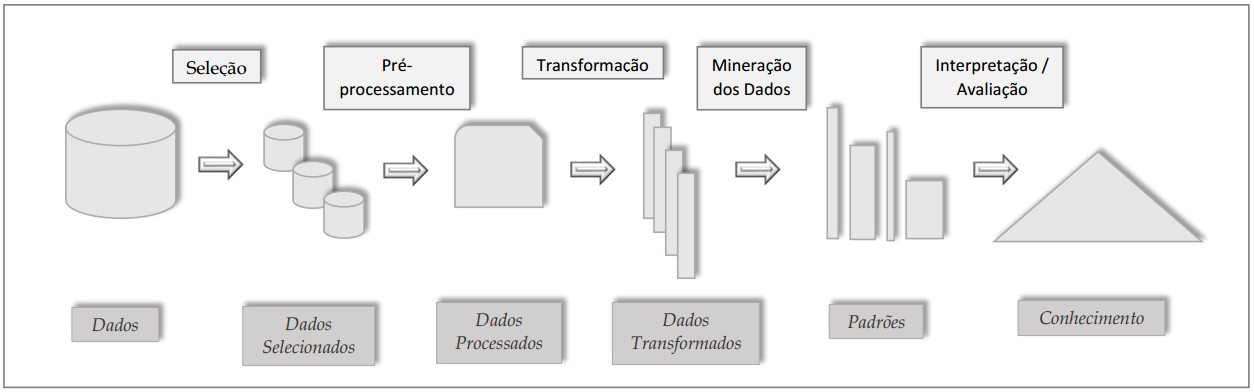
\includegraphics[width=16cm, height=6cm]{images/fases-kdd}}
\caption {Fases do Processo de Extração de Conhecimento (KDD)~\cite{fayyad1996}.}
\label{fayaad_kdd}
\end{figure}

\begin{itemize}
\item \textit{Seleção:} A fase de seleção diz a respeito à análise da disponibilidade e relevância dos dados. É nessa etapa que ocorre a seleção do conjunto ou subconjunto de variáveis ou amostras de dados, onde o processo de descoberta será executado;

\item \textit{Pré-processamento:} A fase de pré-processamento consiste na filtragem e limpeza dos dados. Os processos de filtragem e limpeza visam a remoção de dados inconsistentes, redundantes, valores faltantes ou extremos, que possam interferir nos resultados ou que sejam irrelevantes durante a mineração; 

\item \textit{Transformação:} A fase de transformação consiste na formatação  adequada dos dados, para que os algoritmos possam ser aplicados corretamente. Segundo \citet{han_kamber2006}, a fase de transformação pode envolver as atividades de suavização (remoção de ruídos nos dados),  agregação (sumarização dos dados), generalização (referência por conceitos de fácil entendimento \textit{(alto nível)}), normalização (dimensionamento dos dados em uma faixa de valores) e criação de novos atributos;

\item \textit{Mineração de Dados:} A fase de mineração de dados consiste na exploração e análise dos dados. Nessa fase, são aplicadas as técnicas de mineração de dados, como classificação, sumarização, regressão, clusterização, dentre outras aos atributos, de modo detectar-se padrões de comportamento dos dados e gerar novas descobertas; 

\item \textit{Interpretação e Avaliação:} A fase de interpretação e avaliação, consiste em alcançar propriamente as informações desejadas. Após a finalização da mineração de dados, os resultados obtidos são analisados, sintetizados, avaliados e organizados para apresentação e publicação. 
\end{itemize}

\section{Componentes de um Sistema de Mineração de Dados} \label{3title2}

Segundo \citet{han_kamber2006}, um sistema de mineração de dados é constituído por diversos componentes integrados, conforme a descrição da Figura \ref{componentes}.

\begin{figure}[!htb]
	\centering
	{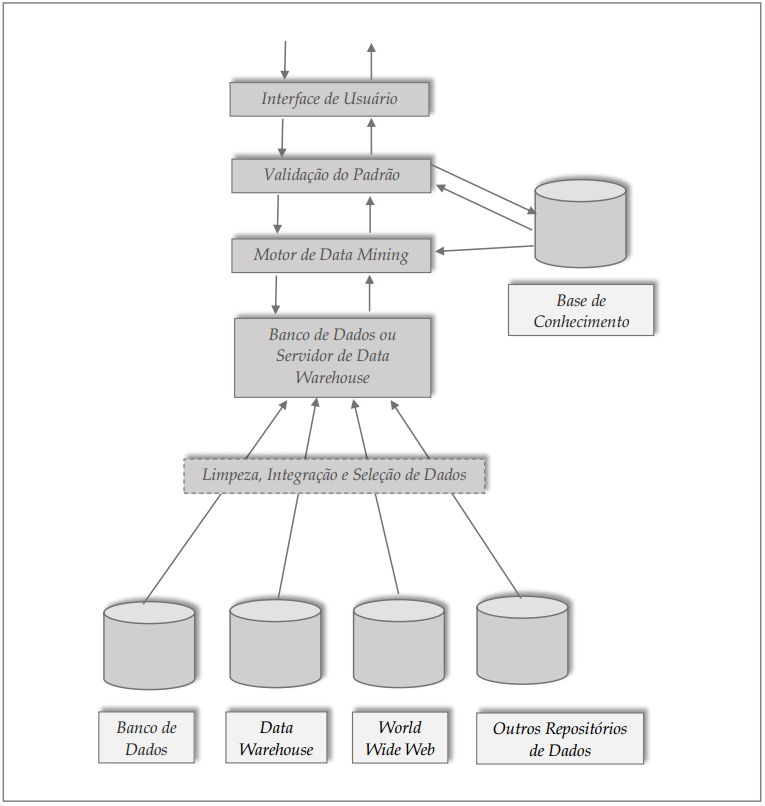
\includegraphics[width=10cm, height=11cm]{images/componentes_mineracao}}
	\caption {Componentes necessários em um sistema de \textit{data mining}~\citep{han_kamber2006}.}
	\label{componentes}
\end{figure}

\begin{itemize}
	\item \textit{Base de aquisição de dados:} podem ser compostos por bancos de dados, \textit{World Wide Web}, repositórios digitais ou \textit{data warehouse};
	
	\item \textit{Servidores de banco de dados ou data warehouse:} tem como função retornar os dados relevantes de acordo com as requisições do usuário;
	
	\item \textit{Base de Conhecimento:} corresponde ao domínio de conhecimento utilizado para orientar a busca dos dados e avaliar os padrões resultantes. Pode fazer uso de hierarquias de conceitos, crenças de usuário, metadados, restrições adicionais ou limites;
	
	\item \textit{Motor de Mineração de Dados:} é essencial na extração de dados. É formado por um conjunto de módulos funcionais que realizam tarefas como caracterização, associação e análise de correlação, classificação, predição, análise de \textit{clusters}, análise de dados ruidosos, entre outras;
	
	\item \textit{Módulo de Avaliação de Padrões:} este componente tem como função empregar medidas e interagir com módulos de mineração de dados com o objetivo encontrar padrões que sejam interessantes (relevantes), sendo possível também utilizar limites para filtrar valores que estejam fora dos padrões. Pode ser integrado ao módulo de mineração de dados, porém deve ser analisado a implementação dos métodos utilizados para mineração de dados;
	
	\item \textit{Interface de Usuário:} este módulo tem por objetivo a comunicação, permitindo a interação entre os usuários e o sistema, dando aos usuários a possibilidade de especificar uma determinada consulta, estabelecer uma tarefa de mineração de dados, inserir informações que aprimorem a pesquisa ou realizar a análise exploratória tomando por base dados intermediários. Entre outras funções, a interface de usuário permite
	a consulta em esquemas de banco de dados, \textit{data warehouse} ou estruturas de dados, avaliar padrões de mineração e visualizar os padrões em formatos diversos.
\end{itemize}

\section{Técnicas de Mineração de Dados} \label{3title3}

Diversas técnicas podem ser empregadas durante o processo de mineração de dados, tais como a classificação, regressão, clusterização, predição, sumarização, detecção de anomalias, dentre outras. Cada técnica fornece uma forma distinta de tratamento e organização dos dados, ficando a critério do avaliador utilizar a(s) que melhor se adequar(em) ao contexto da análise. 

A seguir, serão descritas as técnicas utilizadas na análise de dados neste trabalho, sendo elas a classificação, predição, árvores de decisão, clusterização e detecção de anomalias.

\subsection{Classificação} \label{3subtitle1}

Segundo \citet{han_kamber2006}, classificação é uma forma de análise de dados que extrai modelos que descrevem as classes de dados importantes. \citet{fayyad1996} definem a classificação como a aprendizagem de uma função que mapeia (classifica) um determinado item em uma entre várias classes pré-definidas. \citet[p. 506]{cardoso_machado2008} definem a classificação na mineração de dados como \textit{"o processo de criar modelos (funções) que descrevem e distinguem classes ou conceitos, baseados em dados conhecidos, com o propósito de utilizar esse modelo para predizer a classe de objetos que ainda não foram classificados".}


\citet{han_kamber2006} listam alguns exemplos práticos de classificação na análise de dados. Um agente bancário, durante a realização de um empréstimo, pode utilizar regras de classificação para determinar se um cliente é considerado seguro ou de risco para o banco. O mesmo processo de classificação pode ser utilizado por um gerente de uma loja, para saber o cliente com um determinado perfil pode realizar novas compras; ou por um médico, que pode avaliar dados de determinada doença a fim de prever qual tratamento pode ser mais adequado ou eficaz. 

\citet{han_kamber2006} definem a classificação como um processo de duas etapas. Na primeira fase, um classificador é criado descrevendo o conjunto de dados com classes pré-determinadas, sendo descrito como a \textit{fase de treinamento ou aprendizagem}, onde um algoritmo de classificação cria o classificador analisando ou aprendendo com o conjunto de treinamento. O conjunto de treinamento é uma composição de tuplas geradas pelo banco de dados e seus rótulos de classe associados. Na classificação, uma tupla pode ser constituída por amostras, instâncias, pontos de dados \textit{(data points)} ou objetos de dados. Cada tupla é assumida como pertencente a uma classe pré-definida, sendo determinada pelo atributo do rótulo de classe. Esta etapa também pode ser compreendida como a aprendizagem de um mapeamento ou função pelo classificador (por exemplo, \textit{y = f(t)}, donde \textit{f} pode prever o rótulo de classe \textit{y} de uma determinada tupla \textit{t}).

A segunda etapa consiste na aplicação do classificador sobre o conjunto de dados de teste, composta de tuplas de teste e seus respectivos rótulos de classe. As tuplas de teste são selecionadas aleatoriamente a partir do conjunto de dados geral, e são independentes das tuplas de treinamento, de modo que estas não são usadas na criação do classificador. Nesta etapa, é verificada a precisão (acurácia) do classificador, que é a porcentagem de tuplas do conjunto de testes que foram classificadas corretamente pelo classificador. \citet{han_kamber2006} e  \citet{witten2005} apontam a importância de se mensurar a acurácia do classificador, pois em alguns casos, o classificador pode obter um bom desempenho com dados de treinamento, mas quando aplicado sobre dados de testes, apresentam altas taxas de erro, principalmente quando são analisados dados com algum tipo de ruído (por exemplo, valores desproporcionais ou informados com erro). Caso o classificador apresente resultados considerados satisfatórios, este é considerado apropriado para classificar tuplas de dados cujos rótulos de classes são desconhecidos. 

As duas etapas da classificação são representadas pela Figura \ref{treinamento} (fase de treinamento) e pela Figura \ref{teste} (fase de teste) do classificador sobre as tuplas de dados. 

\begin{figure}[!htb]
	\centering
	{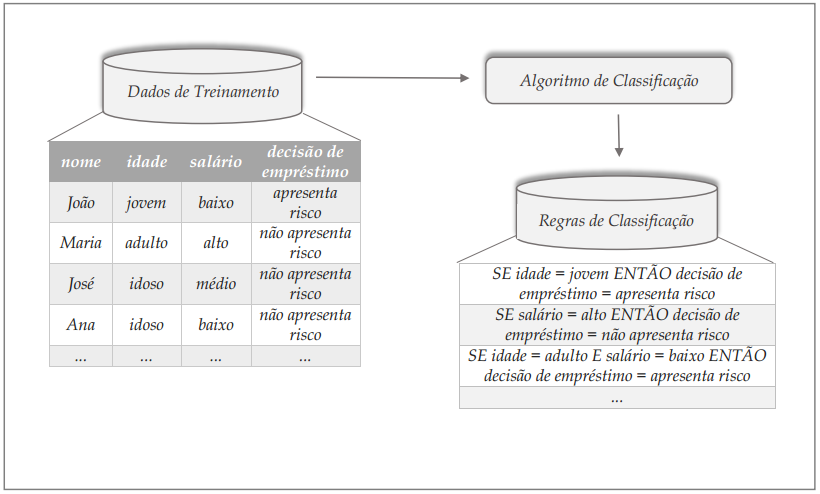
\includegraphics[width=15cm, height=8cm]{images/classificacao1}}
	\caption {Fase de treinamento, onde os dados são analisados por um classificador~\citep{han_kamber2006}.}
	\label{treinamento}
\end{figure}

\begin{figure}[!htb]
	\centering
	{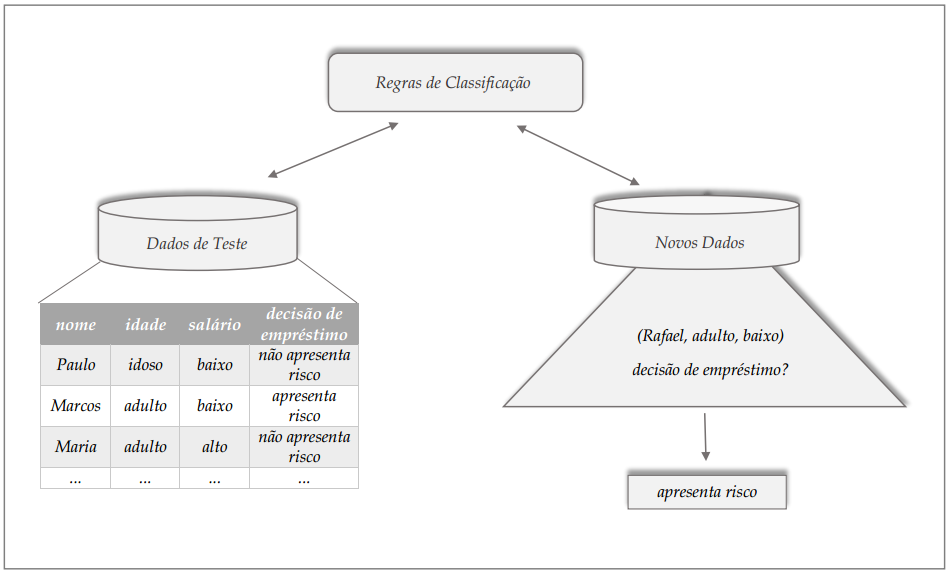
\includegraphics[width=15cm, height=8cm]{images/classificacao2}}
	\caption {Fase de teste, onde os dados de teste são aplicados para estimar a precisão (acurácia) do classificador~\citep{han_kamber2006}.}
	\label{teste}
\end{figure}

\subsubsection{Árvores de Decisão} \label{3subsubtitle3}

Para \citet{coelho_leite}, árvores de decisão são definidas como diagramas elaborados em modo sequencial, baseada em aprendizagem indutiva. \citet{han_kamber2006} definem indução por árvore de decisão como a aprendizagem de árvores de decisão a partir de classes rotuladas nas tuplas de treinamento. A estrutura da árvore de decisão é semelhante a um fluxograma, onde cada nó interno (não-folha) indica um teste de um atributo, cada ramo representa o resultado de um teste e cada nó da folha possui um rótulo de classe. \citet{correa2007} define árvore de decisão como 
\begin{quotation}
	"Uma árvore de decisão é formada por um conjunto de regras de classificação. Cada caminho da raiz até uma folha representa uma destas regras. A árvore de decisão deve ser definida de forma que, para cada observação da base de dados, haja um e apenas um caminho da raiz até a folha." 
\end{quotation}

A Figura \ref{arvore_decisao} apresenta um modelo de árvore de decisão, tomando por base a aprovação do aluno em Computação Básica. Dado que o aluno foi aprovado em Computação Básica, este é classificado como formado. Caso contrário, outras verificações são realizadas na estrutura da árvore, como por exemplo, se o aluno reprovou outras disciplinas. Dada a reprovação do aluno em outras disciplinas,  este é classificado como evadido, e caso contrário, formado.

\begin{figure}[!htb]
	\centering
	{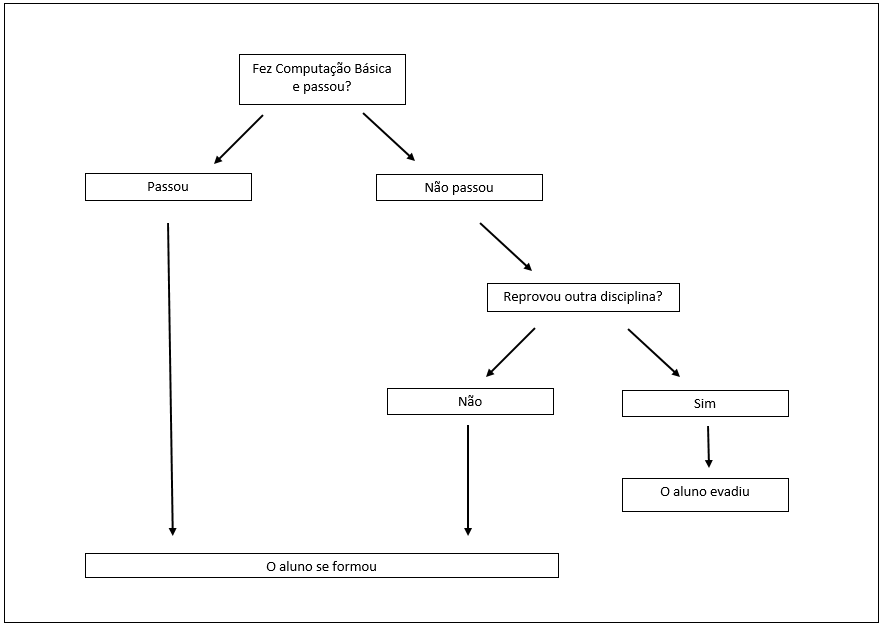
\includegraphics[width=10cm, height=8cm]{images/imagem7}}
	\caption {Exemplo de árvore de decisão.}
	\label{arvore_decisao}
\end{figure}

É importante observar, tomando o exemplo acima, que uma árvore de decisão pode ser usada com dois propósitos: previsão (descobrir se o aluno sairá formado) e descrição (fornecer informações relevantes a respeito da relação entre reprovações na disciplina Computação Básica e o processo de evasão).

Os algoritmos \textit{J48, J48graft} e o \textit{LADTree} são exemplos de algoritmos baseados em árvores de decisão. O algoritmo \textit{J48} gera uma árvore não binária e utiliza uma medida chamada relação de ganho para construir a árvore de decisão, onde o atributo com maior índice de ganho normalizado é tomado como o nó raiz e o conjunto de dados é dividido com base nos valores dos elementos da raiz. O atributo mais relevante é calculado para todos os sub-nós individualmente, e o processo é repetido até que a predição seja concluída. O algoritmo J48 pode lidar com atributos discretos e contínuos, dados de treinamento com valores faltantes e atributos com custos diferentes, além de fornecer uma opção para podar a árvore após sua geração \citep{rajput_arora}. 

O algoritmo \textit{J48graft} é uma versão estendida do J48 que considera a inserção de ramos adicionais para a árvore na fase de pós-processamento. \citet{wisaeng} define a técnica de enxerto como um processo indutivo que adiciona nós inferidos de uma tabela de decisão, com a finalidade de reduzir erros de predição. Ele identifica as regiões no espaço da instância que estão vazias ou contém somente exemplos classificados incorretamente e explora classificações alternativas, considerando diferentes testes que poderiam ter sido selecionados nos nós acima da folha que contém a região em questão \citep{witten2005}. Conforme \citet{rajput_arora}, o propósito é aumentar a probabilidade das instâncias que estão fora do conjunto abrangido pelos dados de treinamento serem classificadas corretamente. Ainda que a árvore torne-se mais complexa, apenas as ramificações (nós) que não introduzam quaisquer erros de classificação em dados já classificados corretamente são considerados.

O algoritmo \textit{LADTree (LAD - Análise Lógica de dados)} é definido por \citet{wisaeng} como um classificador de variável alvo binária, com base na aprendizagem de uma expressão  lógica que pode distinguir amostras positivas e negativas em um conjunto de dados. A construção de um modelo LAD para um conjunto de dados geralmente envolve a geração de amplos padrões estabelecidos e a seleção de um subconjunto que satisfaça a premissa, de modo que cada padrão no modelo satisfaça determinados requisitos em termos de prevalência e homogeneidade. Já \citet{witten2005} descrevem como função do LADTree a construção de multiclasses alternadas de árvores de decisão usando o algoritmo \textit{LogitBoost}.




\subsubsection{Classificação por Regras} \label{3subsubtitle2}

Segundo \citet{han_kamber2006}, a classificação baseada em regras é um modelo representado por um conjunto de regras \textit{'se-então'}, o qual estuda o relacionamento entre itens de dados que ocorrem com frequência, proporcionando a obtenção de associações relevantes em um conjunto de itens aplicados a outros itens e identificando grupos que apresentam uma coocorrência entre si. O condicional \textit{se} de uma regra corresponde ao antecedente da regra ou condição prévia. O condicional \textit{então} corresponde ao resultado da regra. Nas antecedências da regra, a condição pode consistir em um ou mais testes de atributos, e cada regra  pode resultar em uma previsão de classe. A Figura \ref{regras_classificacao} apresenta um exemplo de modelo baseado em regras para classificar um aluno como provável formando em um curso de graduação. A partir dos atributos relacionados à forma de ingresso e idade, foram geradas de regras de classificação para determinar a formatura ou desligamento do aluno.

\begin{figure}[!htb]
	\centering
	{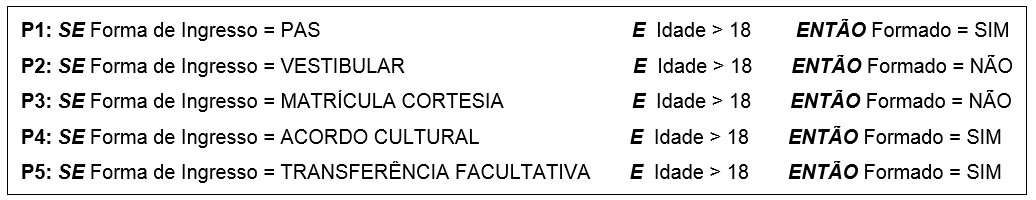
\includegraphics[width=14cm, height=3cm]{images/imagem8}}
	\caption {Exemplo de modelo baseado regras de decisão.}
	\label{regras_classificacao}
\end{figure}

Uma desvantagem apontada por \citet{witten2005} para a geração de regras é o \textit{overfit} (quando o modelo torna-se muito ajustado ao conjunto de dados de treinamento) dos dados de treinamento, não generalizando adequadamente para conjuntos de testes independentes, particularmente em dados ruidosos.  

Os algoritmos \textit{OneR} e \textit{DecisionTable} são exemplos de algoritmos baseados em regras. O algoritmo \textit{OneR}, também conhecido com \textit{1R (uma regra)}, utiliza apenas um dos atributos para realizar a classificação do conjunto de teste. Conforme \citet{zampirolli2014}, o algoritmo consiste, durante a fase de treinamento, em encontrar o atributo que apresente a maior taxa de acerto de classificação das instâncias. Esse algoritmo apresenta um bom desempenho sobre conjunto de dados no qual "um dos atributos é claramente mais importante que o restante, porque seus valores quase sempre darão uma pista de qual deve ser a classificação correta".

O algoritmo \textit{DecisionTable} constrói um classificador com base em tabela de decisão. O algoritmo avalia características de subconjuntos usando pesquisa \textit{best-first} (em tradução livre, primeiro melhor) e pode usar validação cruzada para avaliação. Uma opção utiliza o método \textit{nearest-neighbor} (vizinho mais próximo) para determinar a classe para cada instância que não é abrangida por uma entrada da tabela de decisão, ao invés de utilizar a tabela global, com base no mesmo conjunto de características \citep{witten2005}. 


\subsubsection{Meta-aprendizado} \label{subsubtitle3}

Para \citet[p. 188]{carrier2004}, o  meta-conhecimento consiste em \textit{“qualquer tipo de conhecimento que possa ser extraído da aplicação de um processo de aprendizagem para a resolução de um problema”}. \citet{bezerra2015} definem meta-aprendizado na mineração de dados como uma técnica que visa processar modelos de conhecimento sobre um meta-conhecimento no contexto da mineração de dados. No meta-aprendizado, os algoritmos são ajustados a partir das experiências obtidas de várias aplicações de um algoritmo em fase de treinamento. De acordo com \citet{souza2010}, o meta-aprendizado visa auxiliar a escolha de algoritmos em questões relacionadas a mineração de dados e aprendizagem de máquina, e pode ser utilizado em tarefas de caráter preditivo, tais como classificação. A aplicação do meta-aprendizado em tarefas de classificação é definida como \textit{metaclassificação} \citep{bezerra2015}.

De acordo com \citet{ferrari2014} e \citet{souza2010}, um \textit{meta-exemplo} de treinamento é construído da comparação de um conjunto de algoritmos utilizados em determinado processo de mineração de dados. Cada meta-exemplo é formada por dois conjuntos que armazenam:
\begin{itemize}
	\item (1)- características similares a diferentes instâncias em uma classe (exemplo: número de atributos);
	\item (2)-desempenho dos diferentes algoritmos aplicados ao conjunto de dados.
\end{itemize}

Dado um conjunto de meta-exemplos, um meta-algoritmo é aplicado a fim de verificar as características observadas da mineração e o melhor algoritmo a ser utilizado. O meta-conhecimento obtido sobre os meta-exemplos é utilizado para apontar os algoritmos mais eficientes para situações futuras.

A Figura \ref{meta-classificacao} apresenta o processo simplificado de metaclassificação apresentado por \citet{bezerra2015}. Primeiramente, os classificadores realizam o treinamento no conjunto de dados de treinamento. Em seguida, os classificadores geram predições por meio da análise de um conjunto de teste. A partir do conjunto de teste e das predições geradas, é construído um conjunto de treinamento do meta-nível, e por fim, o metaclassificador gerado é treinado sobre o conjunto de treinamento do meta-nível.

\begin{figure}[!htb]
	\centering
	{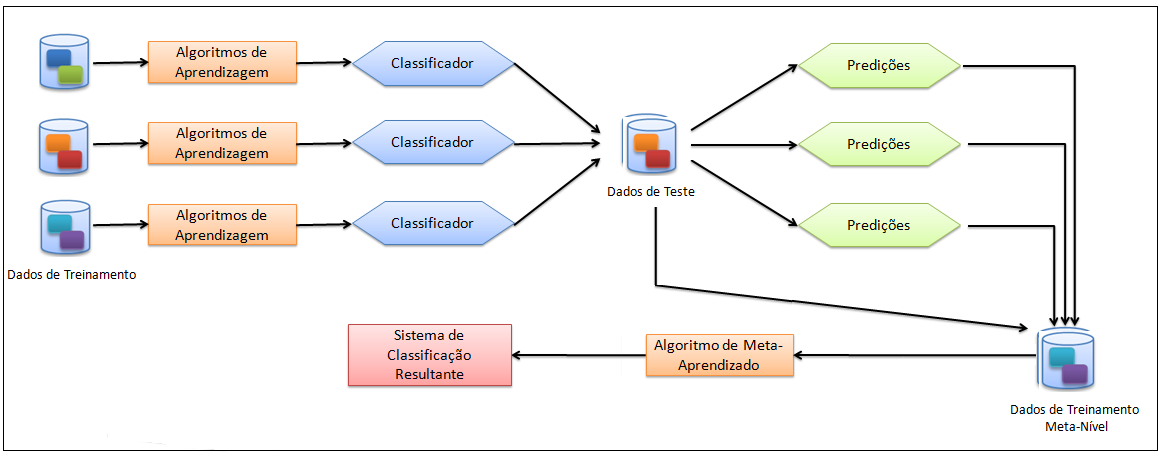
\includegraphics[width=15cm, height=7cm]{images/meta-aprendizado}}
	\caption {Etapas do processo de metaclassificação apresentado por \citet{bezerra2015}.}
	\label{meta-classificacao}
\end{figure}

Os algoritmos \textit{LogitBoost} e \textit{RandomCommittee} são exemplos de algoritmos baseados em meta-aprendizado. O algoritmo \textit{LogitBoost} realiza a regressão logística aditiva. O número apropriado de iterações pode ser determinado por meio de validação cruzada interna \citep{witten2005}. É utilizado para realizar a indução de árvores com modelos de regressão logística linear nas folhas.

O algoritmo \textit{RandomCommittee} constrói um conjunto de classificadores básicos randomicamente e realiza a média de suas previsões. Cada classificador é baseado nos mesmos dados, mas utiliza um número diferente de atributos. Apresenta um bom desempenho desde que a base do classificador seja aleatória, do contrário, todos os classificadores seriam iguais. \citep{witten2005}. 




\subsection{Predição} \label{3subtitle2}

A predição (ou predição numérica) consiste na aplicação de modelos de análise com o objetivo de determinar possíveis valores futuros para um determinado atributo. \citet{han_kamber2006} citam como exemplo um gerente de \textit{marketing} que deseja descobrir quanto um determinado cliente vai gastar durante um processo de venda em uma loja. 

Embora sejam processos similares, vale destacar aqui algumas distinções entre o processo de classificação e predição, conforme apontadas por \citet{han_kamber2006}. Na predição, o classificador consiste em prever valores ordenados, e na classificação rótulos categóricos. A precisão (acurácia), no caso da predição, é estimada calculando o erro com base na diferença entre o valor previsto e o valor efetivo para cada um dos dados do conjunto de teste.

Alguns critérios podem ser levados em consideração para comparar e avaliar os métodos de classificação e predição~\citep{han_kamber2006} a serem utilizados, tais como:
\begin{itemize}
	\item \textit{Acurácia (precisão)}: capacidade de prever corretamente rótulos categóricos ou valores para novos dados;
	
	\item \textit{Velocidade:} referentes aos custos computacionais empregados na geração e utilização de um classificador ou preditor;
	
	\item \textit{Escalabilidade:} capacidade de construir um dado classificador ou preditor de forma eficiente em bases com grandes quantidades de dados;
	
	\item \textit{Robustez:} capacidade de acerto do classificador ou preditor sobre dados com ruídos ou valores faltantes;
	
	\item \textit{Interpretabilidade:} refere-se ao nível de compreensão e entendimento sobre os métodos de classificação e predição. 
\end{itemize}

\subsection{Clusterização} \label{3subtitle4}

Segundo \citet{han_kamber2006}, a clusterização consiste em agrupar um conjunto de objetos, sejam estes físicos ou abstratos, em um grupo de objetos semelhantes. Por sua vez, um \textit{cluster} é definido como um conjunto de objetos de dados que possuem semelhanças entre si e que possuem características distintas em relação a outros conjuntos de objetos, não possuindo classes previamente definidas. A clusterização tem como vantagem a fácil adaptação a mudanças e ajuda a esclarecer características únicas e úteis que possam distinguir diferentes agrupamentos. \citet{han_kamber2006} descrevem que por agrupamento automatizado, é possível identificar regiões densas e esparsas no espaço do objeto, de modo a descobrir padrões globais de distribuição e correlações que sejam interessantes entre os atributos dos dados. A análise de \textit{clusters} pode ser aplicada a vários segmentos, tais como pesquisas de mercado, processamento de imagens e reconhecimento de padrões.

\begin{figure}[!htb]
\centering
{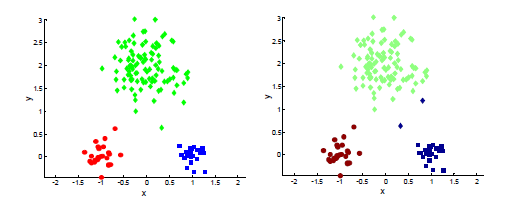
\includegraphics[width=12cm,height=6cm]{images/cluster}}
\caption {Exemplos de agrupamentos de dados \textit{(clusters)}}
\label{cluster}
\end{figure}

Conforme  destacado por \citet{dantas2014}, o processo de clusterização, por vezes, pode ser confundido com o processo de classificação. Na classificação, os objetos são manipulados e distribuídos em classes com características particulares, enquanto que no processo de clusterização os objetos são aglomerados em grupos definidos.

\citet{han_kamber2006} listam alguns requisitos típicos do processo de clusterização em mineração de dados:
\begin{itemize}
\item \textit{Escalabilidade:} muitos algoritmos de clusterização funcionam bem em pequenas bases de dados. No entanto, essas bases também podem conter de centenas a milhares de objetos para análise, o que pode implicar na necessidade de maior desempenho dos algoritmos de análise. Segundo \citet{palmeira_santos2014}, um algoritmo é dito escalável se o tempo de execução do mesmo cresce proporcionalmente ao tamanho do conjunto de dados, considerando os recursos da máquina, como tamanho de memória RAM e processador;

\item \textit{Capacidade de lidar com diferentes tipos de atributos:} os algoritmos devem ser capazes de trabalhar com os mais variados tipos de dados, sejam eles numéricos, nominais, booleanos, dentre outros;

\item \textit{Capacidade de lidar com a alta dimensionalidade dos dados:} um banco de dados pode armazenar registros que contenham várias dimensões ou atributos, o que aumenta o espaço de busca. Dados destas tipologias tornam-se mais difíceis de serem trabalhados, visto que os mesmos podem se encontrar dispersos ou enviesados;

\item \textit{Descobrir \textit{clusters} de forma arbitrária:} muitos algoritmos de agrupamento determinam \textit{clusters} com base em parâmetros de medidas. Baseados nessas medidas, os algoritmos podem reconhecer agrupamentos esféricos com tamanhos e densidades similares. No entanto, um \textit{cluster} pode assumir diferentes formatos, sendo necessário que os algoritmos possam detectar esses agrupamentos de forma arbitrária;

\item \textit{Possuir requisitos mínimos para o domínio de conhecimento para determinar parâmetros de entrada:} os algoritmos geralmente requerem parâmetros de entrada fornecidos pelo usuário para que a análise seja realizada, sendo os resultados  associados aos parâmetros de entrada. Esses parâmetros geralmente são difíceis de serem determinados, principalmente em conjunto de dados que contém objetos de alta dimensão;

\item \textit {Habilidade para lidar com ruídos de dados:} os banco de dados podem fornecer dados com valores extremos, ambíguos ou desconhecidos. Alguns algoritmos, ao trabalhar com estes tipos de dados, tendem a produzir resultados insatisfatórios ou diferentes da realidade;

\item \textit{Possibilitar o agrupamento incremental e insensível à ordem dos registros de entrada:} alguns algoritmos não possibilitam a inserção de novos dados, sendo necessário criar novos agrupamentos. Outros algoritmos são sensíveis à ordem de entrada dos dados, retornando assim agrupamentos diferentes dependendo dos dados de entrada. Daí a importância de algoritmos que sejam incrementais e insensíveis à entrada de novos registros.

\item \textit{Possuir base em restrições de agrupamento:} algumas aplicações trabalhadas no mundo real necessitam de estabelecer restrições sobre os dados, e o principal desafio sobre este aspecto é encontrar agrupamentos de dados que apresentem um bom comportamento sobre as restrições especificadas;

\item \textit{Ser interpretável e utilizável:} os resultados devem ser interpretáveis, compreensíveis e utilizados pelo usuário, onde os agrupamentos estejam relacionados ao contexto das interpretações e aplicações.
\end{itemize}


\subsection{Detecção de Anomalias} \label{3subtitle5}

A detecção de anomalias, também referenciada como detecção de desvios ou análise de \textit{outliers} (valores extremos), visa identificar dados que não se encontram de acordo com os padrões especificados para a mineração, considerados exceções ou ruídos, conforme mostrado na Figura \ref{anomalias}. Estes dados, na maioria das vezes, tendem a impactar de forma negativa os resultados obtidos na mineração de dados.

\begin{figure}[!htb]
\centering
{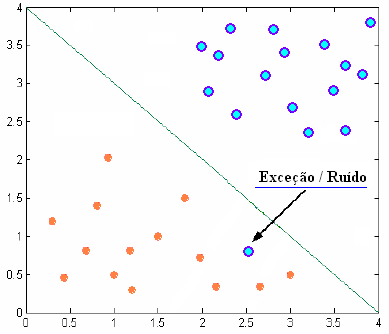
\includegraphics[width=8cm,height=7cm]{images/anomalia}}
\caption {Detecção de anomalia (exceção) no conjunto de dados.}
\label{anomalias}
\end{figure}

A análise e detecção de anomalias permite apresentar novos padrões e alterações de comportamento, tais como atividades suspeitas, potenciais ameaças e possibilidades de fraudes~\citep{witten2005}, contribuindo para o monitoramento e segurança de transações e sistemas. \citet{han_kamber2006} descrevem que no processo de detecção de anomalias, são constituídos modelos de comportamento normal para a rede, que são usados para comparar e identificar novos padrões que se afastam dos perfis pré-definidos. Como vantagem, a detecção de anomalias permite identificar mais claramente ruídos que até então não foram observados, porém apresenta como desvantagem a alta porcentagem de detecção de falsos positivos (por exemplo, uma pessoa saudável é classificada como doente). 

Uma observação importante a ser destacada é que conjunto de regras com muitas especificações também pode induzir o resultado ao erro. Conforme apontado por \citet{miranda2012}, dois aspectos se encaixam nesse cenário: o \textit{overfitting} e o \textit{underfitting}. 

O \textit{overfitting} diz respeito ao alto grau de complexidade dos modelos de regras, apresentando muitos parâmetros relativos ao número de observações. Nestes casos, pode-se ajustar o algoritmo para apresentar um alto grau de precisão para dados conhecidos. Porém, quando aplicados em novos dados, estes tendem a diminuir a precisão dos resultados. \citet{miranda2012} destaca que em situações de \textit{overfitting}, altas taxas de erros são identificadas no retorno dos dados utilizados na base de teste. 

Em contrapartida, o \textit{underfitting} pode ser resultado de um modelo que é demasiadamente simplificado, de tal forma que o algoritmo não consegue se ajustar aos dados. Assim, a probabilidade do algoritmo apresentar altas taxas de erro aumenta, tanto no conjunto de treinamento como no de teste. Ambos os casos devem ser analisados com cautela, pois podem interferir diretamente nos resultados obtidos pelo pesquisador.

\section{\textit{Softwares} para Mineração de Dados} \label{3title4}

No mercado, existem várias ferramentas proprietárias e \textit{open source}\footnote{\textit{Open Source} é o termo utilizado para designar \textit{softwares} de código aberto.}  que auxiliam na mineração de dados, desde a fase de pré-processamento até a visualização dos resultados obtidos. A seguir, serão explanados previamente alguns dos \textit{softwares} abertos que podem ser encontrados e baixados pela Internet \textit{(download)}.

\begin{itemize}

\item \textit{R:} É uma linguagem e ao mesmo tempo um ambiente para a realização de computação que envolvam cálculos estatísticos e gráficos. É semelhante a linguagem S, desenvolvida pela Bell Laboratories (antiga AT \& T, agora Lucent Technologies), embora sejam consideradas diferentes em termos de implementação~\footnote{\url{http://http://www.r-project.org/about.html}}. R fornece uma série de técnicas gráficas e estatísticas (modelos lineares e não-lineares, classificação, clusterização, análise de séries temporais, entre outras) que são altamente extensíveis. Pode ser utilizada e difundida por profissionais de diversas áreas de atuação, tais como economia, medicina e ciência da computação, devido à sua quantidade de materiais bibliográficos disponíveis na Internet. Uma das facilidades oferecidas pelo R é a disponibilização de símbolos e fórmulas matemáticas disponíveis que facilitam na geração e publicação de relatórios. Sua estrutura conta com um conjunto integrado que permite a manipulação e armazenamento de dados, contém operadores para cálculos em tabelas, ferramentas para análise de dados, instalações gráficas que permitem a visualização dos dados em tela ou de forma impressa, além de sua linguagem de programação permitir o uso de condicionais, funções recursivas, estruturas de repetição e manipulação de entrada e saída de dados. É uma ferramenta que está disponível para diferentes plataformas, como Windows, Mac OS e Unix (incluindo o FreeBSD e o Linux).

\item \textit{RapidMiner:} O RapidMiner~\footnote{ \url{https://rapidminer.com/}} é um \textit{software} produzido pela empresa com o mesmo nome, que fornece um conjunto integrado de aplicações que permitem a mineração de dados. É utilizado nos mais diversos contextos, tais como aplicações comerciais, bem como para a investigação, educação, formação, a modelagem e desenvolvimento de aplicativos, e provê suporte para todas as etapas do processo de mineração de dados, incluindo a visualização, otimização e validação dos resultados. Assim como para a mineração de dados, o RapidMiner pode ser aplicado para a aprendizagem de máquina, mineração de textos, análise preditiva e análise de negócios. Este se encontra disponíveis em versões pagas (\textit{Personal Edition} e \textit{Profissional Edition}), e na versão gratuita (\textit{Starter Edition}), que é mais limitada em recursos disponibilizados.

\item \textit{Pentaho:} Pentaho é um \textit{software} desenvolvido em Java, desenvolvido em 2004 pela Pentaho Corporation~\footnote{\url{http://www.pentaho.com/}}. É fortemente utilizado para aplicações que envolvam inteligência empresarial. Sua estrutura é composta por diversos componentes, que permitem realizar a extração, transformação e carregamento dos dados; mineração, análise de \textit{clusters}, processamento de grandes bases de dados; geração de relatórios e metadados.
\end{itemize}

Além das ferramentas listadas acima, outra que é amplamente utilizada no processo de mineração de dados é o \textbf{Weka}, a ser abordada mais detalhadamente na próxima seção, e que será a ferramenta base para o processo de mineração de dados a ser desenvolvido neste trabalho.

\section{\textit{Software} Weka} \label{3title5}

\textit{Weka} é uma abreviação para Waikato Environment for Knowledge Analisys, (em tradução livre, Ambiente Waikato para Análise do Conhecimento), desenvolvido pela Universidade de Waikato, localizada na Nova Zelândia. O \textit{software} é composto por algoritmos de aprendizagem de máquina e uma coleção de recursos que realizam o pré-processamento, regressão, classificação, clusterização, aplicação de regras de visualização dos dados e apresentação de resultados~\citep{weka}. A ferramenta é desenvolvida utilizando a linguagem de programação Java e sua distribuição segue os termos da GNU \textit{(General Public Licence, ou Licença Pública Geral)}. 

O Weka apresenta uma variedade de recursos e ferramentas, como amplo suporte a todas as etapas do processo experimental de mineração de dados, desde a preparação dos dados de entrada, análise estatística de esquemas de aprendizagem até a visualização dos dados e apresentação dos resultados. Possui uma variedade de algoritmos de treinamento e ferramentas de pré-processamento, que são apresentadas em uma interface amigável ao usuário, além de possibilitar a integração direta com bancos de dados, o que permite ao usuário obter os dados direto da base e salvá-los em formato adequado para uso posterior no Weka. Outra vantagem é que a ferramenta é de distribuição livre e multiplataforma, funcionando em diferentes sistemas operacionais, como Windows, Linux e Mac OS. A Figura \ref{weka} apresenta a interface de usuário inicial do Weka.

\begin{figure}[!htb]
	\centering
	{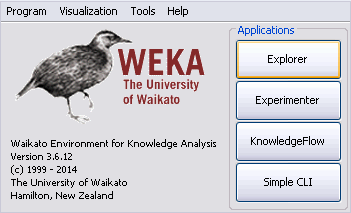
\includegraphics[width=9cm,height=6cm]{images/weka}}
	\caption {Interface inicial do Weka.}
	\label{weka}
\end{figure}


De acordo com \citet{witten2005}, o Weka pode ser trabalhado utilizando as interfaces gráficas \textit{Explorer}, \textit{Experimenter} e \textit{KnowledgeFlow}. 

A interface \textit{Explorer}, mostrada na Figura \ref{modo1}, oferece ao usuário a possibilidade de acesso às opções existentes na barra de menu, assim como possibilita ao usuário carregar os dados a serem utilizados e a verificar os resultados gerados pelos algoritmos de mineração. Porém, uma das desvantagens do modo \textit{Explorer} é que todo o conjunto de dados utilizado é mantido em memória, limitando-se a problemas de pequeno e médio porte.

\begin{figure}[!htb]
	\centering
	{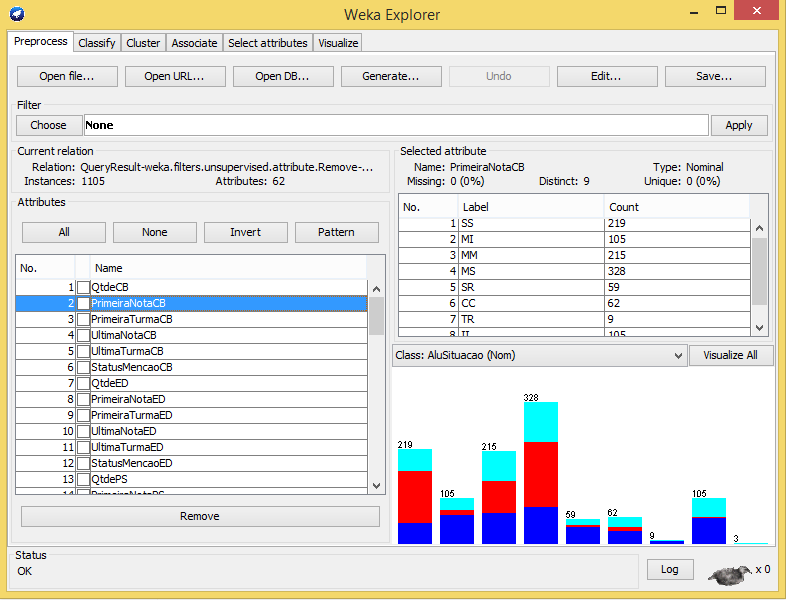
\includegraphics[width=10cm,height=7cm]{images/modo1}}
	\caption {Captura de tela da interface \textit{Explorer} do Weka.}
	\label{modo1}
\end{figure}


A interface \textit{KnowledgeFlow}, mostrada na Figura \ref{modo2}, permite a criação de configurações para o processamento de fluxo de dados. Pela interface gráfica do \textit{KnowledgeFlow}, é possível arrastar caixas que representam os algoritmos de aprendizagem e fontes de dados ao redor da tela, e juntá-los na configuração desejada. Também permite especificar um fluxo de dados por componentes conectados que representam  as fontes de dados, ferramentas de pré-processamento, algoritmos de mineração, métodos de avaliação e módulos de visualização.

\begin{figure}[!h]
	\centering
	{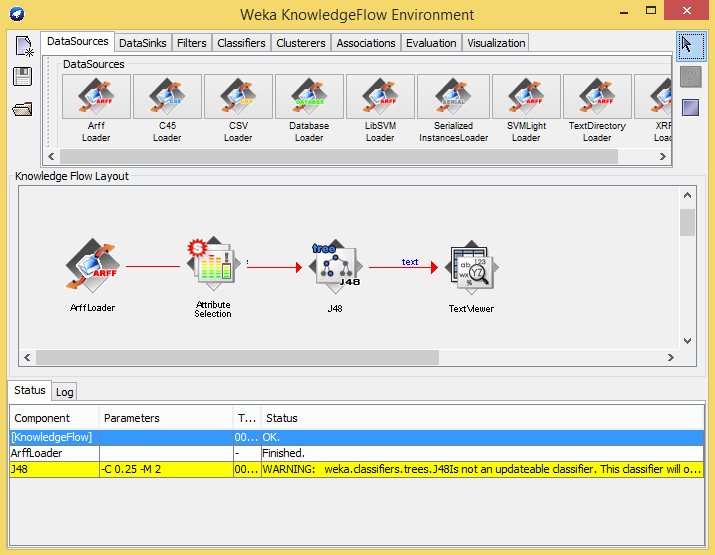
\includegraphics[width=10cm,height=7cm]{images/modo2}}
	\caption {Captura de tela da interface \textit{KnowledgeFlow} do Weka.}
	\label{modo2}
\end{figure}

A opção \textit{Experimenter}, mostrada na Figura \ref{modo3}, tem por objetivo facilitar a identificação de quais métodos e parâmetros nas técnicas de classificação e regressão são mais adequados para determinado problema. A interface foi desenvolvida com o intuito de facilitar ao usuário a comparação de várias técnicas de aprendizagem, tornando mais fácil a execução de classificadores e filtros com diferentes definições de parâmetros sobre um conjunto de dados, a coleta de estatísticas de desempenho e a execução de testes significativos. 

\begin{figure}[!htb]
	\centering
	{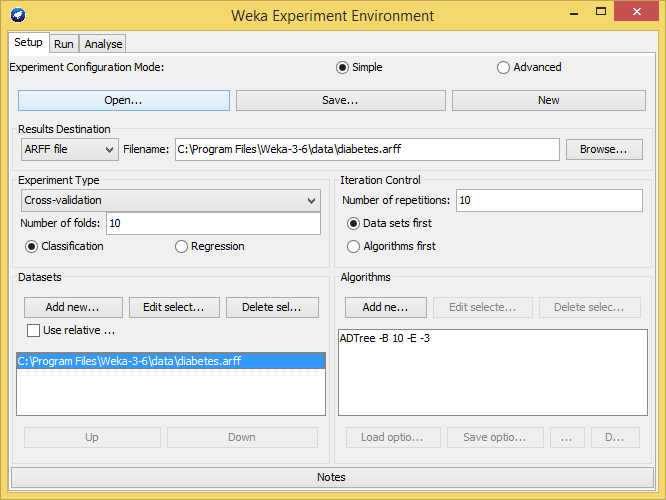
\includegraphics[width=10cm,height=7cm]{images/modo3}}
	\caption {Captura de tela da interface \textit{Experimenter} do Weka.}
	\label{modo3}
\end{figure}
 

Outra possibilidade, além das três interfaces apresentadas anteriormente, é utilizar o Weka pela interface \textit{Simple CLI}, mostrada na Figura \ref{modo4}. A opção \textit{Simple CLI} apresenta dicas de como utilizar o Weka por linha de comando (via \textit{Terminal} no Linux ou \textit{Prompt de Comando} no Windows), e permite ao usuário informar os comandos a serem utilizados na mesma janela.

\begin{figure}[!htb]
	\centering
	{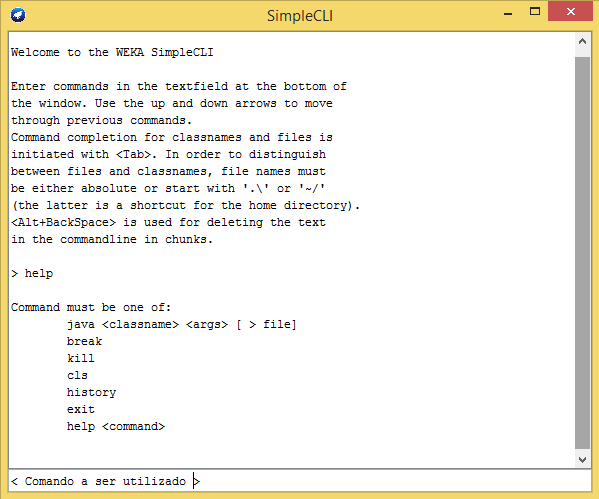
\includegraphics[width=10cm,height=7cm]{images/modo4}}
	\caption {Captura de tela da interface \textit{Simple CLI} do Weka.}
	\label{modo4}
\end{figure}
 
 
  
\chapter{Mineração de Dados dos Alunos de Ciência da Computação da UnB} \label{chapter5}

Neste capítulo, será descrita a metodologia utilizada para a análise dos dados e obtenção dos resultados propostos, orientado pelo processo de extração do conhecimento (KDD) descrito no Capítulo \ref{chapter3}.

Na Seção \ref{5title1}, é delimitado o objeto de pesquisa, que consiste dos objetivos a serem alcançados pela mineração de dados. A Seção \ref{5subtitle1} descreve a etapa de aquisição e seleção dos dados, além ferramentas utilizadas para armazenamento e manipulação desses dados. A Seção \ref{5subtitle2} descreve a etapa de pré-processamento dos dados, listando os atributos que foram removidos da mineração. A Seção \ref{5subtitle3} descreve a etapa de transformação dos dados, que envolve a modificação e criação de atributos e tabelas, além de descrever o processo de criação dos arquivos de dados a serem minerados pelo Weka. Finalizando, a Seção \ref{5subtitle4} descreve a etapa de mineração dos dados, que envolve a análise dos dados com os algoritmos de mineração e a seleção dos algoritmos utilizados para a análise dos dados.

\section{Delimitação do Objeto de Pesquisa} \label{5title1}

Da abordagem realizada nas Seções \ref{2title53} e \ref{2title54}, é possível identificar alguns aspectos em comum nos trabalhos de \citet{dantas2014} e \citet{palmeira_santos2014}, tais como:

\begin{itemize}
	\item Os três primeiros semestres são os que registram as maiores taxas de evasão;
	\item As disciplinas de Computação Básica e Estruturas de Dados apresentam altas taxas de reprovação;
	\item As disciplinas de Matemática e Física, tais como Cálculo 1, Cálculo 2, Cálculo 3, Física 1, Física 2 e Física 3 apresentam altas taxas de reprovação;
	\item Das disciplinas ofertadas pelo CIC-UnB, Computação Básica e Estruturas de Dados estão entre as disciplinas consideradas determinantes para a continuidade ou não do curso, por serem obrigatórias dos semestres iniciais e por serem pré-requisitos para as disciplinas subsequentes;
	\item Entre as formas de evasão, a maioria ocorre por abandono de curso.
\end{itemize}

Diante dos aspectos apresentados, a análise consistirá de dados sobre os alunos do curso de Bacharelado em Ciência da Computação e seus respectivos históricos acadêmicos. 

Entre as disciplinas a serem analisadas, foram selecionadas Computação Básica, Estruturas de Dados e Programação Sistemática (CIC-UnB); Cálculo 1, Cálculo 2 e Cálculo 3 (MAT-UnB); Física 1, Física 2 e Física 3 (IF-UnB). Essas disciplinas estão distribuídas entre o primeiro e terceiro semestre do fluxo acadêmico, e são consideradas disciplinas de base para a continuidade do curso. 

Neste trabalho a mineração de dados terá a finalidade de:
\begin{itemize}
	\item Verificar as variáveis que influenciaram no processo de evasão ao longo dos semestres;
	\item Identificar regras que permitam justificar a evasão para alunos de determinado semestre;
	\item Verificar se menções ou turmas das disciplinas analisadas exercem influência sobre o processo de evasão;
	\item Identificar os principais padrões e tendências que permitam justificar a evasão dos alunos ao longo dos anos.
\end{itemize}

Uma vez definidos os objetivos a serem alcançados pela mineração de dados, a próxima etapa consiste na implementação das fases do processo extração do conhecimento (KDD), conforme explicitado na Seção \ref{3title1} do Capítulo \ref{chapter3}. As Seções \ref{5subtitle1} até \ref{5subtitle4} detalham todo o processo de mineração de dados empregado neste trabalho, com a finalidade de alcançar os objetivos propostos.


\section{Seleção dos Dados} \label{5subtitle1}

Os dados obtidos para este trabalho foram os mesmos utilizados por \citet{palmeira_santos2014}, que foram recuperados do Sistema de Informação Acadêmica de Graduação (SIGRA) e disponibilizados pelo Decanato de Planejamento e Orçamento da Universidade de Brasília (DPO). Os arquivos de dados foram entregues em formato \textit{CSV} (disponibilizados pelo DPO) e \textit{SQL} (disponibilizados por \citet{palmeira_santos2014}). Junto aos arquivos, foi entregue um dicionário de dados, a fim de facilitar a compreensão do significado dos valores numéricos para determinados atributos. 

Com o objetivo de otimizar a busca e recuperação dos registros, optou-se por trabalhar com os arquivos em formato SQL, visto que os registros já se encontravam pré-processados para serem manipulados via banco de dados. 

O banco de dados escolhido para este trabalho foi o MySQL versão 5.5.12, e como ferramenta de apoio à edição de tabelas e dados foi escolhido o HeidiSQL versão 9.2.0~\footnote{\url{http://www.heidisql.com/}}, mostrado na Figura \ref{heidisql}, devido a disponibilidade de recursos para tratamento de dados, por possuir uma interface simples e intuitiva (disponível no idioma português brasileiro), por disponibilizar um guia de ajuda para a utilização dos comandos da linguagem SQL e por ser uma ferramenta gratuita para \textit{download}. O HeidiSQL pode ser utilizado com os bancos de dados MySQL, Microsoft SQL Server e PostgreSQL.

\begin{figure}[!htb]
	\centering
	{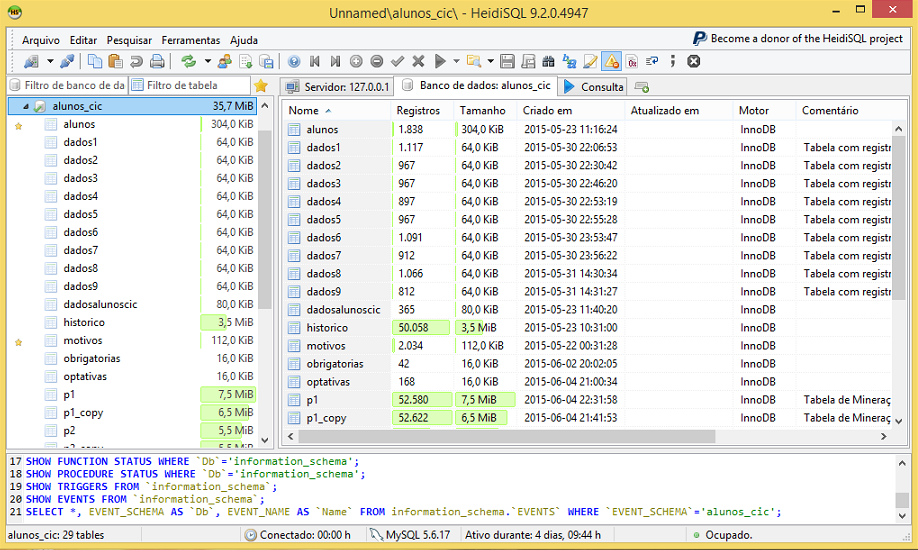
\includegraphics[width=13cm,height=8cm]{images/heidisql}}
	\caption {Interface do HeidiSQL.}
	\label{heidisql}
\end{figure}

\begin{figure}[!htb]
	\centering
	{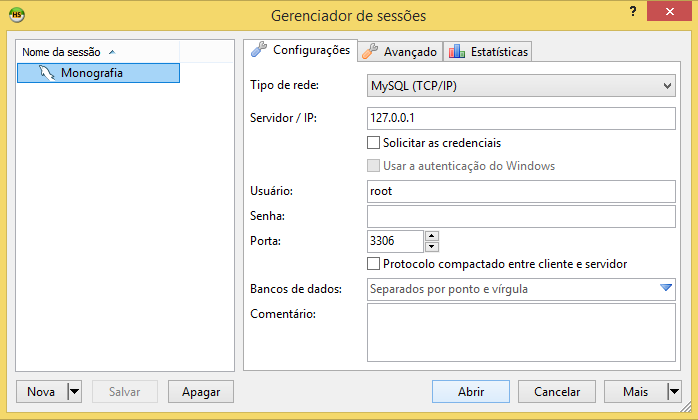
\includegraphics[width=11cm,height=7cm]{images/heidisqlinicio}}
	\caption {Tela de configuração de conexão no HeidiSQL.}
	\label{heidisqlinicio}
\end{figure}


Para manipular bases, tabelas e dados no MySQL via HeidiSQL, é necessário que o servidor do banco de dados esteja ativo. Ao executar o HeidiSQL, aparecerá a tela de configuração da conexão, conforme mostrado na Figura \ref{heidisqlinicio}. Na opção \textit{Tipo de Rede} é possível escolher o banco de dados a ser utilizado (\textit{MySQL (TCP/IP)}). O campo \textit{Servidor IP} requer o endereço IP do servidor ao qual o MySQL está vinculado (neste caso é utilizado o endereço local da máquina \textit{127.0.0.1}). Os campos \textit{Usuário, Senha} e \textit{Porta} são referentes às credencias de acesso ao banco de dados, sendo padrão o campo \textit{Usuário} como \textit{"root"}, o campo \textit{Senha} em branco (nula) e o campo \textit{Porta} como \textit{3306}.

Primeiramente, foi criada uma nova base de dados \textit{(database)}, denominada \textit{alunos\_cic}, onde foram armazenadas as tabelas criadas. Após a execução dos arquivos SQL, foram criadas quatro tabelas principais no MySQL, sendo estas:
\begin{itemize}
	\item \textit{Alunos:} Contém os dados gerais sobre os alunos ingressantes entre o primeiro semestre de 1983 e o primeiro semestre de 2014. Ao todo, foram contabilizados 2034 registros. Os atributos referentes estão descritos na Tabela \ref{5tab};
	\begin{longtable}{c|c}
		
		\caption{Atributos referentes aos alunos.} 	\label{5tab}\\
		\hline
		Atributos & Descrição\\
		\hline
			MatricAluno & Código do aluno no sistema\\
			AnoIngresso & Ano de ingresso na Universidade\\
			FormaIngresso & Forma de ingresso na Universidade\\
			SemestreIngresso & Semestre de ingresso na Universidade\\
			AnoSaida & Ano de saída da Universidade\\
			SemestreSaida & Semestre de Saída da Universidade\\
			FormaSaida & Forma de Saída da Universidade\\
			PerIngressoOpcao & Período de ingresso na opção\\
			SemestreIngressoOpcao & Semestre de ingresso na opção\\ 
			ForIngressoOpcao & Forma de ingresso na opção\\
			PerSaidaOpcao & Período de saída da opção\\
			SemestreSaidaOpcao & Semestre de saída na opção\\
			ForSaidaOpcao & Forma de saída da opção\\
			AlunoRegistrado & Se aluno está registrado ou não\\
			PeriodoCurricular & Ano do período curricular\\
			SemestrePeriodoCurricular & Semestre do período curricular\\
			AluSexo & Sexo do aluno\\
			AluNacionalidade & Nacionalidade do aluno\\
			AluDtNasc & Data de nascimento do aluno\\
			AluCotId & Sistema de ingresso do aluno\\
			AluEscola & Tipo de escola que o aluno cursou o Ensino Médio\\
		\hline
	\end{longtable}
	\item \textit{Histórico:} Contém todos os registros de histórico acadêmico dos alunos entre o ano de 2000 e 2013. Ao todo, foram contabilizados 52.900 registros. Os atributos referentes estão descritos na Tabela \ref{5tab1};
		\begin{longtable}{c|c}
			
			\caption{Atributos referentes ao histórico.} 	\label{5tab1}\\
			\hline
			Atributos & Descrição\\
			\hline
			MatricAluno & Código do aluno no sistema\\
			Ano & Ano em que a disciplina foi cursada\\
			Semestre & Semestre em que a disciplina foi cursada\\
			CodDisc & Código da Disciplina\\
			Créditos & Quantidade de créditos da disciplina\\
			Mencao & Menção obtida pelo aluno\\
			Frequencia & Quantidade de faltas, em porcentagem\\		
			\hline
		\end{longtable}
	\item \textit{Obrigatórias:} Contém informações sobre as disciplinas obrigatórias do curso. Ao todo, foram contabilizados 42 registros. Os atributos referentes estão descritos na Tabela \ref{5tab2};
	\begin{longtable}{C{4cm}|C{7cm}}
		
		\caption{Atributos referentes as disciplinas obrigatórias.} 	\label{5tab2}\\
		\hline
		Atributos & Descrição\\
		\hline
		CodDisciplina & Código da disciplina\\
		NomeDisciplina & Nome da disciplina\\
		Departamento & Departamento que oferta a disciplina\\	
		Fluxo & Semestre que a disciplina é ofertada\\	
		\hline
	\end{longtable}
	\item \textit{Optativas:} Contém informações sobre as disciplinas optativas do curso. Ao todo, foram contabilizados 168 registros. Os atributos referentes estão descritos na Tabela \ref{5tab3}.
	
		\begin{table}[!htb]
			\centering
			\caption{Atributos referentes as disciplinas optativas.} 	\label{5tab3}
			\begin{tabular}{C{3cm}|C{6cm}}
				\hline
				Atributos & Descrição\\
				\hline
				CodDisciplina & Código da disciplina\\
				NomeDisciplina & Nome da disciplina\\
				\hline
			\end{tabular}
		\end{table}
\end{itemize}

\section{Pré-processamento dos Dados} \label{5subtitle2}

Após a criação das tabelas \textit{Alunos}, \textit{Histórico}, \textit{Obrigatórias} e \textit{Optativas} no banco de dados, foi realizada uma análise a fim de identificar e remover os atributos considerados desnecessários, redundantes ou inconsistentes para o processo de mineração. Os atributos listados abaixo foram removidos, em sua maioria, por apresentarem informações redundantes ou por não serem úteis o alcance dos objetivos definidos na Seção \ref{5title1}.

Da tabela \textit{Alunos}, por apresentarem informações redundantes, foram removidos:
\begin{center}
	\textit{PerIngressoOpcao, SemestreIngressoOpcao, ForIngressoOpcao, PerSaidaOpcao, SemestreSaidaOpcao, ForSaidaOpcao, AlunoRegistrado, PeriodoCurricular, SemestrePeriodoCurricular, AluNacionalidade.}
\end{center}


Da tabela \textit{Histórico}, por não ser utilizado, foi removido:

\begin{center}
 \textit{Frequencia.}
\end{center}


Da tabela \textit{Obrigatórias}, por não serem utilizados, foram removidos:

\begin{center}
	\textit{Departamento, Fluxo.}
\end{center}


A tabela \textit{Optativas}, neste caso, foi removida completamente, visto que o foco da mineração está nas disciplinas obrigatórias dos três primeiros semestres, sendo desnecessário o seu uso.


\section{Transformação dos Dados} \label{5subtitle3}

Para facilitar a compreensão dos atributos, foram necessárias algumas modificações nas tabelas \textit{Obrigatórias} e \textit{Alunos}, além da criação de novas tabelas e atributos (colunas) no banco de dados, a serem descritas ao decorrer desta Seção.

Na tabela \textit{Obrigatórias}, a chave primária é definida pelo campo \textit{codDisciplina}, que é do tipo numérico, visto que cada disciplina possui seu próprio código. Como cada código de disciplina é composto por seis algarismos numéricos, torna-se mais difícil para o usuário identificar intuitivamente a qual disciplina o código se refere. Para facilitar a identificação das disciplinas pelo usuário, foi criado um novo atributo denominado \textit{sigla}, que é uma abreviação do nome da disciplina, composta de 3 a 5 caracteres. Para cada disciplina na tabela \textit{Obrigatorias}, foi criada uma sigla distinta. A Tabela \ref{novaObr} mostra a nova estruturação dos atributos da tabela \textit{Obrigatórias} no MySQL. A lista de disciplinas obrigatórias e suas respectivas abreviações estão disponíveis no Apêndice \ref{apendiceA}.

\begin{table}[!h]
		\caption{Nova estrutura da tabela \textit{Obrigatórias}.} 	\label{novaObr}
		\centering
	\begin{tabular}{C{4cm}|C{8cm}}
	\hline
	Coluna & Descrição\\
	\hline
	CodDisciplina & Código da disciplina\\
	NomeDisciplina & Nome da disciplina\\
	Sigla & Abreviação do nome da disciplina\\	
	\hline
		\end{tabular}
\end{table}


Na tabela \textit{Alunos}, foram realizadas algumas modificações nos atributos numéricos, que foram convertidos para valores nominais e vice-versa. Com base no dicionário de dados fornecidos junto aos arquivos de dados, os valores numéricos dos atributos \textit{FormaIngresso, FormaSaida, AluEscola} e \textit{AluCotId} foram substituídos por suas respectivas descrições. As Tabelas \ref{atualiza1}, \ref{atualiza2}, \ref{atualiza3} e \ref{atualiza4} apresentam as conversões realizadas para forma de ingresso, forma de saída, tipo de escola e tipo de cota dos alunos, baseado nos dados registrados nas tabela.

\begin{table}[!h]
	\caption{Atualização de valores para o atributo \textit{FormaIngresso}.} 	
	\label{atualiza1}
	\centering
	\begin{tabular}{C{1cm}|C{5cm}|C{8cm}}
		\hline
		Valor & Convertido para & Nomenclatura Completa\\
		\hline
		0 & Nao Informado & Não Informado\\
		1 & Vestibular &  Vestibular\\	
		2 & Trans Obrigatoria & Transferência Obrigatória\\
		3 & Trans Facultativa & Transferência Facultativa\\
		4 & Port Dipl Curso Superior & Portador de Diploma de Curso Superior\\
		5 & Acordo Cultural & Acordo Cultural-PEC\\
		6 & Convenio Intern & Convênio Internacional\\	
		7 & Matricula Cortesia & Matrícula Cortesia\\
		17 & Pas & Programa de Avaliação Seriada\\	
		20 & Convenio Andifes & Convênio Andifes\\
		24 & Pec-G Pepppfol & \\
		27 & Enem & Exame Nacional do Ensino Médio\\
		\hline
		\end{tabular}
	\end{table}
	
	
	\begin{table}[!h]
		\caption{Atualização de valores para o atributo \textit{FormaSaida}.} 	
		\label{atualiza2}
		\centering
		\begin{tabular}{C{1cm}|C{5cm}|C{8cm}}
			\hline
			Valor & Convertido para & Nomenclatura Completa\\
			\hline
			0 & Cursando & Cursando\\
			1 & Formatura & Formatura\\		
			3 & Desl Jubilamento & Desligamento por Jubilamento\\
			5 & Desl Forca de Convenio & Desligamento por Força de Convênio\\
			6 & Transferencia & Transferência\\	
			7 & Desl Voluntario & Desligamento Voluntário\\
			9 & Falecimento & Falecimento\\	
			12 & Desl Decisao Judicial & Desligamento por Decisão Judicial\\
			16 & Desl Abandono & Desligamento por Abandono\\
			17 & Desl Nao Cumpriu Condicao & Desligamento por não Cumprir Condição\\
			20 & Reprovou 3 Vezes Msm Disc Obr & Reprovou 3 Vezes a Mesma Disciplina Obrigatória\\
			21 & Novo Vestibular & Novo Vestibular\\
			\hline
		\end{tabular}
	\end{table}
	
		\begin{table}[!h]
			\caption{Atualização de valores para o atributo \textit{AluEscola}.} 	
			\label{atualiza3}
			\centering
			\begin{tabular}{C{2cm}|C{4cm}|C{5cm}}
				\hline
				Valor & Convertido para & Nomenclatura Completa\\
				\hline
				\"\#NULO!\" & Nao Informado & Não Informado\\
				0 & Nao Informado & Não Informado\\
				1 & Publica & Escola Pública\\	
				2 & Particular& Escola Particular\\	
				\hline
			\end{tabular}
		\end{table}
		
			\begin{table}[!h]
				\caption{Atualização de valores para o atributo \textit{AluCotId}.} 	
				\label{atualiza4}
				\centering
				\begin{tabular}{C{1cm}|C{6cm}|C{7cm}}
					\hline
					Valor & Convertido para & Nomenclatura Completa\\
					\hline
					0 & Universal & Universal\\
					1 & Negro & Negro\\	
					3 & Escola Publ Baixa Renda PPI & Escola Pública Baixa Renda PPI\\
					4 & Esc Publ Baixa Renda Nao PPI & Escola Pública Baixa Renda Não PPI\\
					5 & Escola Publ Alta Renda PPI & Escola Pública Alta Renda PPI\\
					6 &	Esc Publ Alta Renda Nao PPI & Escola Pública Alta Renda Não PPI\\
					\hline
				\end{tabular}
			\end{table}
	

	Após a conversão dos atributos numéricos em nominais, foi realizado um \textit{inner join}\footnote{O comando \textit{inner join} realiza a correspondência (junção) e retorna os dados de duas ou mais tabelas, desde que haja campos ou chaves correspondentes entre as tabelas.} das tabelas \textit{Alunos} e \textit{Histórico}, e os valores obtidos dessa junção foram salvos em uma nova tabela, denominada \textit{evasao\_todas}. 
	
	Além dos campos obtidos pela junção das tabelas, foram acrescentados três novos atributos na tabela \textit{evasao\_todas}, sendo estes \textit{AluSituacao}, \textit{DiscMateriaCursada} e {DiscStatusMencao}.
	
	 O atributo \textit{AluSituacao}  foi criado para definir a condição atual do aluno: \textit{"Formado"} caso o valor na coluna \textit{FormaSaida} seja "Formatura";  \textit{"Cursando"} caso o valor na coluna \textit{FormaSaida} seja "Cursando"; e \textit{"Desligado"} para os demais valores em \textit{FormaSaida}. 
	 
	 O atributo \textit{DiscMateriaCursada} foi criado com o objetivo de sintetizar os atributos \textit{Sigla} (tabela \textit{Obrigatórias}), \textit{Ano, Semestre} e \textit{Turma} (tabela \textit{Histórico}) em um único valor, por meio da função \textit{concat}~\footnote{A função \textit{concat} na linguagem SQL permite realizar a concatenação de diferentes valores em um único resultado.} no MySQL. 
	 
	 O atributo \textit{DiscStatusMencao} foi criado para identificar se o aluno foi aprovado ou reprovado em determinada disciplina com base na menção obtida. De acordo com as regras da Universidade de Brasília, ao cursar uma disciplina, o aluno poderá obter uma das seguintes menções classificadas conforme a Tabela \ref{mencoes1}.
	
		\begin{table}[!h]
			\caption{Classificação das Menções na Universidade de Brasília.} 	
			\label{mencoes1}
			\centering
			\begin{tabular}{C{2cm}|C{5cm}|C{3cm}}
				\hline
			Menção & Descrição & Nota\\
				\hline
				SR & Sem Rendimento & 0\\	
				II & Inferior & 0,1 a 2,9\\
				MI & Médio Inferior & 3,0 a 4,9\\
				MM & Médio & 5,0 a 6,9\\
				MS & Médio Superior & 7,0 a 8,9\\
				SS & Superior & 9,0 a 10,0\\
				\hline
			\end{tabular}
		\end{table}

	Caso o aluno tenha obtido menção MM, MS, SS ou CC (Crédito Concedido) para determinada disciplina, o valor do atributo \textit{DiscStatusMencao} é \textit{"Aprovado"}. Caso tenha obtido, SR, II ou MI ou tenha realizado o trancamento da disciplina, seja este parcial ou geral (TR, TJ, TM)~\footnote{TJ:Trancamento Parcial de Matrícula. Excepcional e Justificado; TR: Trancamento Parcial de Matrícula. Concessão Automática; TM: Trancamento Geral de Matrícula. Automático e justificado.} o valor do atributo \textit{DiscStatusMencao} é \textit{"Reprovado"}.
	
	Por último, os valores para o atributo \textit{DtNasc} também foram modificados, convertidos de nominais para numéricos. Da data de nascimento dos alunos, foram desprezados os valores do dia e do mês, considerando-se somente o ano.
	
	Após a criação e edição dos atributos na tabela \textit{evasao\_todas}, foi realizada uma cópia da mesma, incluindo os valores dos dados, e salva no banco de dados como \textit{evasao\_obrigatorias}. Nessa nova tabela, foram removidos os dados referentes às disciplinas optativas, visto que estes dados não serão objeto de análise para este trabalho.    
	
	\subsection{Organização dos Dados por Departamento e Disciplinas} \label{5subsubtitle1}
	
	Além das tabelas \textit{evasao\_todas} e \textit{evasao\_obrigatorias}, foram criadas outras três tabelas: \textit{evasao\_cic}, \textit{evasao\_mat} e \textit{evasao\_fis}, contendo dados sobre as disciplinas organizadas por departamento. A tabela \textit{evasao\_cic} contém dados de Computação Básica, Estruturas de Dados e Programação Sistemática; a tabela \textit{evasao\_mat} contém dados de Cálculo 1, Cálculo 2 e Cálculo 3; e  a tabela \textit{evasao\_fis} contém dados de Física 1, Física 2 e Física 3, que foram as disciplinas definidas na Seção \ref{5title1}.  
	
	Para realizar a recuperação e armazenamento dos dados, foi desenvolvido uma aplicação em Java (vide Apêndice \ref{apendiceB}) e executada na IDE~\footnote{IDE - \textit{Integrated Development Environment}, ou \textit{Ambiente Integrado de Desenvolvimento.}} Eclipse, capaz de contar a quantidade de vezes que determinada disciplina foi cursada, recuperar a primeira e última menção obtida pelo aluno, e recuperar a primeira e última turma na qual a disciplina foi cursada da tabela \textit{historico}. Tomando por base a disciplina pré-requisito do primeiro semestre de cada departamento, o método captura as informações para as disciplinas subsequentes, conforme mostrado na Figura \ref{metodoJava}. Por exemplo, a partir dos alunos que cursaram Computação Básica, foram verificados os registros para os alunos que cursaram Estruturas de dados; e a partir dos alunos que cursaram Estruturas de Dados, foram verificados os registros para os alunos que cursaram Programação Sistemática. 
	
	
	
	\begin{figure}[!htb]
		\centering
		{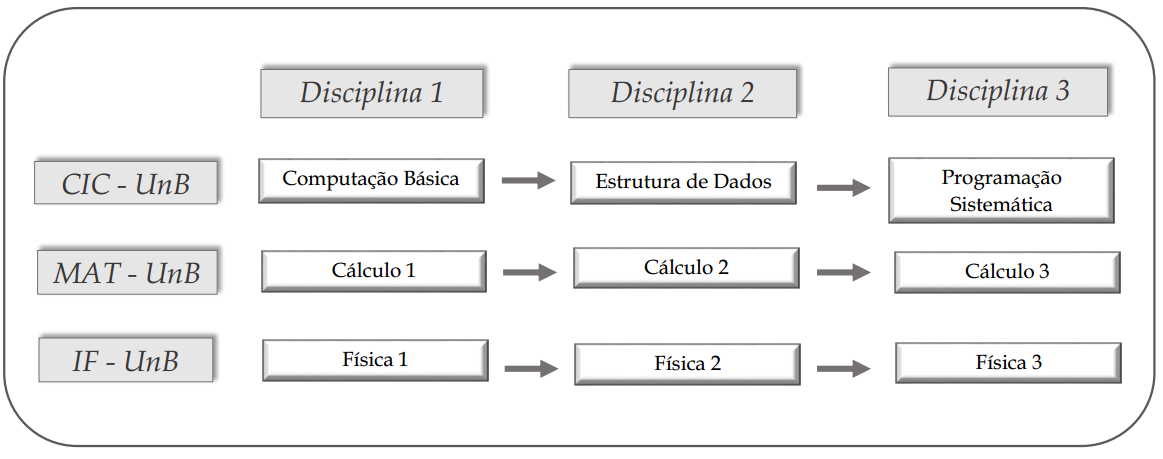
\includegraphics[width=10cm, height=4cm]{images/analiseJava}}
		\caption {Fluxo de Análise das Disciplinas pela aplicação Java. A partir da disciplina pré-requisito do primeiro semestre de cada departamento, foi verificado o histórico do aluno para as disciplinas subsequentes.}
		\label{metodoJava}
	\end{figure}
	
		\begin{figure}[!htb]
			\centering
			{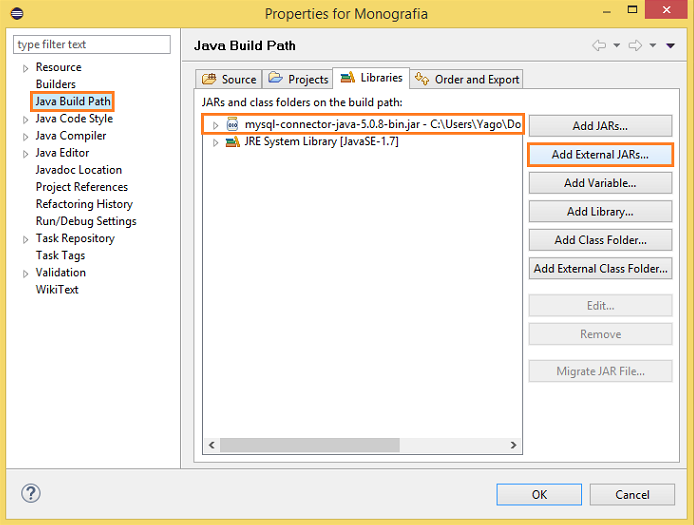
\includegraphics[width=12cm, height=7cm]{images/driverEclipse}}
			\caption {Adicionando o \textit{driver} JBDC ao Projeto no Eclipse.}
			\label{driverJBDC}
		\end{figure}
	
	Para realizar a integração entre o MySQL e a IDE Eclipse, foi necessário baixar o \textit{driver} JBDC~\footnote{O driver pode ser obtido em \url{http://dev.mysql.com/downloads/connector/j/5.1.html}.} do MySQL. Após a obtenção do \textit{driver}, o mesmo foi adicionado à biblioteca do projeto que contém o método utilizado, clicando com o botão direito sobre a pasta do projeto no Eclipse e em seguida selecionando a opção \textit{Properties}. Na nova janela aberta, foi selecionada a opção \textit{Java Build Path} e em seguida a opção \textit{Add External JARs}, conforme mostrado na Figura \ref{driverJBDC}. O \textit{driver} consiste em um arquivo em formato JAR \textit{(Java Archive)}. Com o \textit{driver} JBDC adicionado ao projeto, tornou-se possível realizar consultas SQL e atualizações de tabelas via código Java. 
	
	
	As estruturas de \textit{evasao\_cic, evasao\_mat} e \textit{evasao\_fis} são representadas pelas Tabelas \ref{evasao-cic}, \ref{evasao-mat} e \ref{evasao-fis}. Para cada aluno registrado, foram recuperados a quantidade de vezes que a disciplina foi cursada, a primeira e última nota obtida para a disciplina e a primeira e última turma na qual a disciplina foi cursada, além do \textit{status} da última menção obtida pelo aluno \textit{(aprovado/reprovado)}.

	
		\begin{longtable}{C{4cm}|C{12cm}}
			\caption{Estrutura da Tabela \textit{evasao\_cic}.} 	\label{evasao-cic}\\
				\hline
				Coluna & Descrição\\
				\hline
				Matricula & Matrícula do aluno no sistema\\
				QtdeCB & Quantidade de vezes que Computação Básica foi cursada\\
				PrimeiraNotaCB & Primeira nota obtida em Computação Básica\\
				PrimeiraTurmaCB & Primeira turma cursada de Computação Básica\\
				UltimaNotaCB & Última nota obtida em Computação Básica\\
				UltimaTurmaCB & Última turma cursada de Computação Básica\\
				StatusMencaoCB & Aprovação ou Reprovação do aluno ao cursar Computação Básica pela última vez\\
				QtdeED & Quantidade de vezes que Estruturas de Dados foi cursada\\
				PrimeiraNotaED & Primeira nota obtida em Estruturas de Dados\\
				PrimeiraTurmaED & Primeira turma cursada de Estruturas de Dados\\
				UltimaNotaED & Última nota obtida em Estruturas de Dados\\
				UltimaTurmaED & Última turma cursada de Estruturas de Dados\\
				StatusMencaoED & Aprovação ou Reprovação do aluno ao cursar Estruturas de Dados pela última vez\\
				QtdePS & Quantidade de vezes que Programação Sistemática foi cursada\\
				PrimeiraNotaPS & Primeira nota obtida em Programação Sistemática\\
				PrimeiraTurmaPS & Primeira turma cursada de Programação Sistemática\\
				UltimaNotaPS & Última nota obtida em Programação Sistemática\\
				UltimaTurmaPS & Última turma turma cursada de Programação 
				Sistemática\\
				StatusMencaoPS & Aprovação ou Reprovação do aluno ao cursar Programação Sistemática pela última vez\\
				\hline
		\end{longtable}
	
		\begin{longtable}{C{4cm}|C{12cm}}
			\caption{Estrutura da Tabela \textit{evasao\_mat}.} \label{evasao-mat}\\
			\hline
			Coluna & Descrição\\
			\hline
			Matricula & Matrícula do aluno no sistema\\
			QtdeC1 & Quantidade de vezes que Cálculo 1 foi cursada\\
			PrimeiraNotaC1 & Primeira nota obtida em Cálculo 1\\
			PrimeiraTurmaC1 & Primeira turma cursada de Cálculo 1\\
			UltimaNotaC1 & Última nota obtida em Cálculo 1\\
			UltimaTurmaC1 & Última turma cursada de Cálculo 1\\
			StatusMencaoC1 & Aprovação ou Reprovação do aluno ao cursar Cálculo 1 pela última vez\\
			QtdeC2 & Quantidade de vezes que Cálculo 2 foi cursada\\
			PrimeiraNotaC2 & Primeira nota obtida em Cálculo 2\\
			PrimeiraTurmaC2 & Primeira turma cursada de Cálculo 2\\
			UltimaNotaC2 & Última nota obtida em Cálculo 2\\
			UltimaTurmaC2 & Última turma cursada de Cálculo 2\\
			StatusMencaoC2 & Aprovação ou Reprovação do aluno ao cursar Cálculo 2 pela última vez\\
			QtdeC3 & Quantidade de vezes que Cálculo 3 foi cursada\\
			PrimeiraNotaC3 & Primeira nota obtida em Cálculo 3\\
			PrimeiraTurmaC3 & Primeira turma cursada de Cálculo 3\\
			UltimaNotaC3 & Última nota obtida em Cálculo 3\\
			UltimaTurmaC3 & Última turma turma cursada de Cálculo 3\\
			StatusMencaoC3 & Aprovação ou Reprovação do aluno ao cursar Cálculo 3 pela última vez\\
			\hline
		\end{longtable}
		
				\begin{longtable}{C{4cm}|C{12cm}}
					\caption{Estrutura da Tabela \textit{evasao\_fis}.} \label{evasao-fis}\\
						\hline
						Coluna & Descrição\\
						\hline
						Matricula & Matrícula do aluno no sistema\\
						QtdeF1 & Quantidade de vezes que Física 1 foi cursada\\
						PrimeiraNotaF1 & Primeira nota obtida em Física 1\\
						PrimeiraTurmaF1 & Primeira turma cursada de Física 1\\
						UltimaNotaF1 & Última nota obtida em Física 1\\
						UltimaTurmaF1 & Última turma cursada de Física 1\\
						StatusMencaoF1 & Aprovação ou Reprovação do aluno ao cursar Física 1 pela última vez\\
						QtdeF2 & Quantidade de vezes que Física cursada\\
						PrimeiraNotaF2 & Primeira nota obtida em Física 2\\
						PrimeiraTurmaF2 & Primeira turma cursada de Física 2\\
						UltimaNotaF2 & Última nota obtida em Física 2\\
						UltimaTurmaF2 & Última turma cursada de Física 2\\
						StatusMencaoF2 & Aprovação ou Reprovação do aluno ao cursar Física 2 pela última vez\\
						QtdeF3 & Quantidade de vezes que Física 3 foi cursada\\
						PrimeiraNotaF3 & Primeira nota obtida em Física 3\\
						PrimeiraTurmaF3 & Primeira turma cursada de Física 3\\
						UltimaNotaF3 & Última nota obtida em Física 3\\
						UltimaTurmaF3 & Última turma turma cursada de Física 3\\
						StatusMencaoF3 & Aprovação ou Reprovação do aluno ao cursar Física 3 pela última vez\\
						\hline
				\end{longtable}

\subsection{Geração dos Arquivos em Formato ARFF} \label{5subsubtitle2}

Após a criação das tabelas e organização dos dados, foi necessária a conversão dos registros armazenados no MySQL para o formato ARFF \textit{(Attribute-Relation File Format,} ou \textit{Arquivo em Formato Atributo-Relação}), que é o formato padrão utilizado pelo Weka para realização da mineração de dados \citep{witten2005}. Segundo \citet{witten2005}, o arquivo em formato ARFF apenas fornece o conjunto de dados, não especificando quais atributos devem ser utilizados para classificação. O mesmo arquivo ARFF pode ser utilizado para analisar a forma como cada atributo pode ser classificado a partir de outros atributos, encontrar regras de associação ou identificar agrupamentos \textit{(clusters)}.

 Uma das possibilidades de criar arquivos de dados em formato ARFF é através do próprio Weka, por meio de integração entre o \textit{software} e o MySQL. Da mesma forma que o Eclipse, o Weka requer o \textit{driver} JBDC do MySQL para possibilitar a conexão ao banco de dados.

\subsubsection{Integrando o Weka ao MySQL} \label{sub51}

Para configurar o Weka no sistema operacional \textit{Windows}, torna-se necessária a realização dos seguintes procedimentos:
\begin{itemize}
	\item Salve o \textit{driver} do MySQL na pasta do projeto Weka; 
	\item Na pasta do Weka, clique com o botão direito do mouse sobre o arquivo \textit{weka.jar (Executable Jar File)}, e em seguida, escolha a opção \textit{Abrir com o WinRAR}. Caso não utilize o \textit{WinRAR}, pode-se optar por outro descompactador de arquivos e pastas;
	
	 \begin{figure}[!h]
	 	\centering
	 	{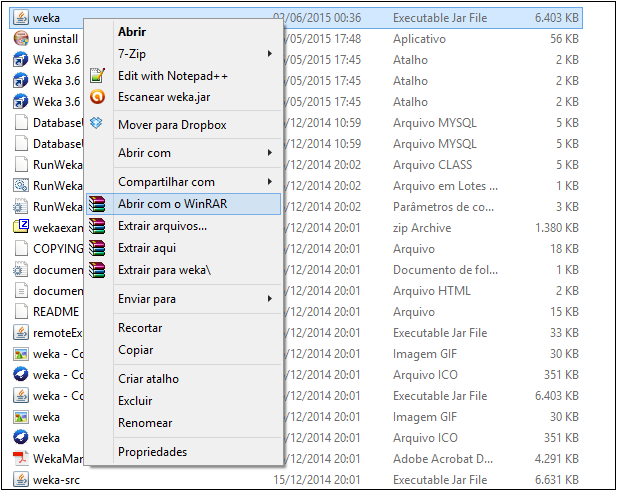
\includegraphics[width=11cm, height=8cm]{images/winrar}}
	 	\caption {Acesso ao arquivo \textit{weka.jar} para configurar a integração entre o Weka e o MySQL.}
	 	\label{winrar}
	 \end{figure}
	 
	 \item Ao abrir o arquivo \textit{weka.jar} com o \textit{WinRAR}, aparecerá um diretório contendo três pastas, sendo estas \textit{java\_cup, META-INF} e \textit{Weka}. Selecione a pasta \textit{Weka}, e em seguida a pasta \textit{experiment}. Na pasta \textit{experiment}, abra o arquivo \textit{DataBaseUtilsmysql.props} com o auxílio de algum editor de textos (Notepad++, Bloco de Notas, Wordpad...), conforme mostrado na Figura \ref{winrar2};
	 
	   \begin{figure}[!h]
	   	\centering
	   	{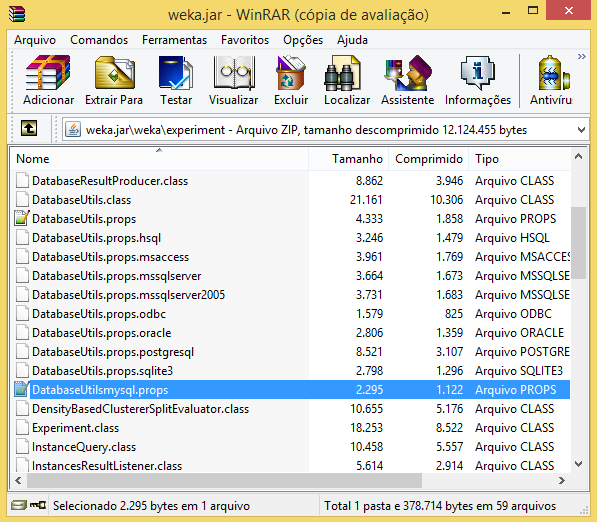
\includegraphics[width=11cm, height=8cm]{images/winrar2}}
	   	\caption {Diretório de acesso ao arquivo \textit{DataBaseUtilsmysql.props} }
	   	\label{winrar2}
	   \end{figure}
	   
	   \item Após abrir o arquivo com o editor de textos, informe o \textit{driver} utilizado do MySQL no campo \textit{jdbcDriver}, e a URL de acesso ao banco de dados no campo \textit{jdbcURL}, conforme mostrado na Figura \ref{winrar3}. Para este trabalho, o \textit{driver} do MySQL utilizado foi o \textit{com.mysql.jdbc.Driver};
	   
	    \begin{figure}[!h]
	    	\centering
	    	{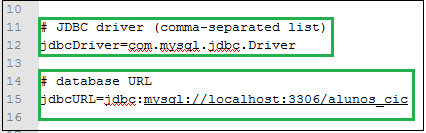
\includegraphics[width=9cm, height=3cm]{images/winrar3}}
	    	\caption {Declaração do \textit{driver} utilizado do MySQL e da URL de acesso ao banco de dados no arquivo \textit{DataBaseUtilsmysql.props.}}
	    	\label{winrar3}
	    \end{figure}
	    
	   \item Na seção \textit{specific data types} do arquivo \textit{DataBaseUtilsmysql.props}, são declarados os tipos de dados a serem utilizados. Para este trabalho, foram utilizados dados do tipo \textit{INT, INTEGER, FLOAT} e \textit{LONG} para dados do tipo númerico, \textit{VARCHAR} e \textit{TEXT} para dados do tipo texto, e \textit{BIT} para dados do tipo binário, conforme mostrado na Figura \ref{winrar4};
	   
	        \begin{figure}[!h]
	        	\centering
	        	{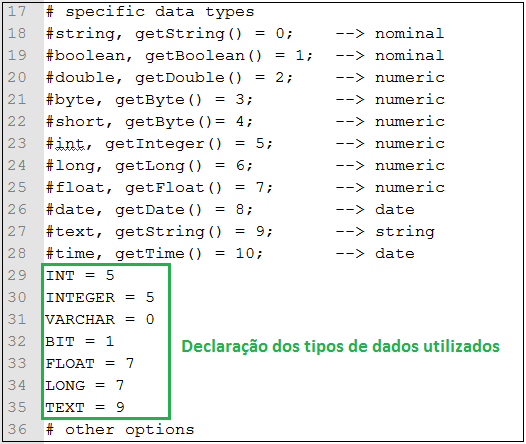
\includegraphics[width=10cm, height=7cm]{images/winrar4}}
	        	\caption {Declaração do \textit{driver} utilizado do MySQL e da URL de acesso ao banco de dados no arquivo \textit{DataBaseUtilsmysql.props.}}
	        	\label{winrar4}
	        \end{figure}
	   
	   \item Salve o arquivo após as modificações realizadas. Em seguida, renomeie-o para \textit{DataBaseUtils.props}, dentro da própria pasta;
	   
	   \item Realizada a alteração no arquivo, execute o Weka via \textit{Prompt de Comando}. Para executar o Weka junto ao MySQL, informe o seguinte comando:
	   \newline
	   \begin{center}
	   	\textit{java -cp <caminho do \textit{driver} MySQL na pasta Weka>; <caminho do diretório do arquivo \textit{weka.jar}> weka.gui.GUIChooser}
	   \end{center}
	   
	   O comando \textit{-cp} é utilizado pelo Java para indicar quais diretórios devem ser pesquisados para encontrar as bibliotecas necessárias para que o programa seja executado \citep{tutorial_weka}. Os diretórios devem ser separados por ponto e vírgula. Um exemplo é mostrado na Figura \ref{winrar5}. Ao executar o comando, o Weka iniciará automaticamente;
	   
	   \begin{figure}[!h]
	   	\centering
	   	{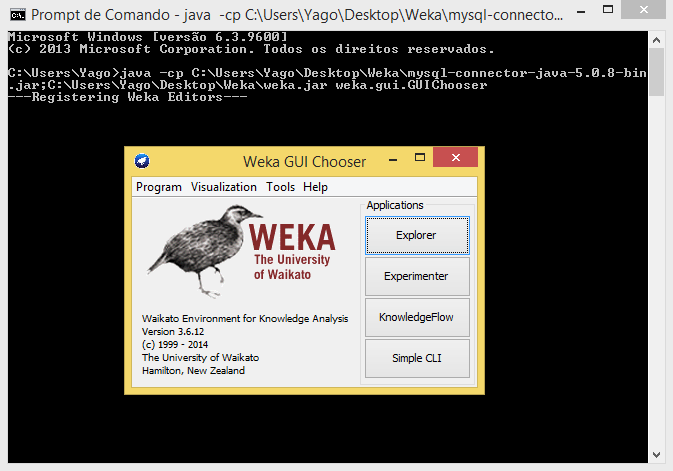
\includegraphics[width=13cm, height=10cm]{images/winrar5}}
	   	\caption {Iniciando o Weka e o MySQL via \textit{Prompt de Comando} do \textit{Windows}.}
	   	\label{winrar5}
	   \end{figure}
	   
	   \item Realizados os procedimentos de configuração, o Weka poderá ser iniciado normalmente pelo atalho \textit{Weka 3.6}.
\end{itemize}
 
\subsubsection{Recuperação dos Dados pelo Weka e Transformação para o Formato ARFF}

Após a configuração do Weka para integrar-se ao MySQL descrita na Seção \ref{sub51}, os arquivos em formato ARFF foram gerados a partir dos seguintes procedimentos:

\begin{itemize}
	\item Abrir o Weka em modo \textit{Explorer};
	\item Na guia de menus, escolher a opção \textit{Open DB...};
	\item No campo \textit{URL}, informar a URL de acesso a base de dados, e em seguida, escolher a opção \textit{User...};
	\item Ao abrir a janela \textit{Database Connection Parameters}, informar a URL de acesso ao banco de dados e as permissões de acesso, conforme mostrado na Figura \ref{weka5};
	
	 \begin{figure}[!h]
	 	\centering
	 	{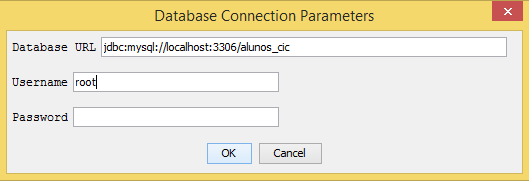
\includegraphics[width=8cm, height=2cm]{images/weka5}}
	 	\caption {Permissões de acesso ao banco de dados no Weka}
	 	\label{weka5}
	 \end{figure}
	
	\item  Em seguida, escolher a opção \textit{Connect}. Caso a conexão seja estabelecida, aparecerá a mensagem \textit{connecting to: <base de dados> =true};
	\item Informe a \textit{query} a ser utilizada e clique na opção \textit{Execute}. Após o retorno dos dados da consulta, clique em \textit{OK}. Os dados serão mostrados no Weka conforme apresentação da Figura \ref{weka6};
	
		 \begin{figure}[!h]
		 	\centering
		 	{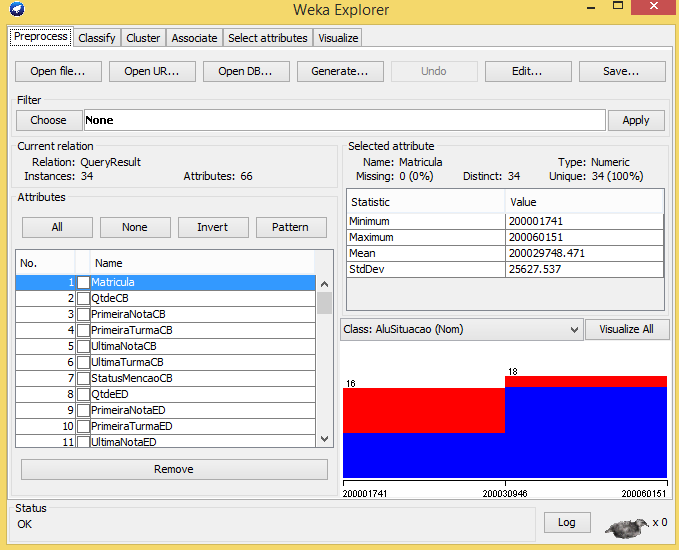
\includegraphics[width=10cm, height=9cm]{images/weka6}}
		 	\caption {Dados recuperados do SQL mostrados no Weka.}
		 	\label{weka6}
		 \end{figure}
	
	\item Agora, basta escolher a opção \textit{Save...} que o arquivo será salvo em formato ARFF.
\end{itemize}

Os procedimentos descritos nesta Seção foram realizados para os dados gerais dos alunos (todos os alunos que possuem histórico no departamento entre 2000 e 2013), e para os dados gerais dos alunos separados por semestre entre 2000 e 2013. Ao todo, foram criados 29 arquivos em formato ARFF. As \textit{querys} utilizadas para criação dos arquivos estão disponíveis no Apêndice \ref{apendiceC}.

Cada arquivo ARFF é composto dos seguintes atributos, conforme mostrado na Tabela \ref{arff}.

	\begin{longtable}{C{4cm}|C{12cm}}
		\caption{Atributos presentes no arquivo ARFF.} \label{arff}\\
		\hline
		Coluna & Descrição\\
		\hline
		Matricula & Matrícula do aluno no sistema\\
		QtdeCB & Quantidade de vezes que Computação Básica foi cursada\\
		PrimeiraNotaCB & Primeira nota obtida em Computação Básica\\
		PrimeiraTurmaCB & Primeira turma cursada de Computação Básica\\
		UltimaNotaCB & Última nota obtida em Computação Básica\\
		UltimaTurmaCB & Última turma cursada de Computação Básica\\
		StatusMencaoCB & Aprovação ou Reprovação do aluno ao cursar Computação Básica pela última vez\\
		QtdeED & Quantidade de vezes que Estruturas de Dados foi cursada\\
		PrimeiraNotaED & Primeira nota obtida em Estruturas de Dados\\
		PrimeiraTurmaED & Primeira turma cursada de Estruturas de Dados\\
		UltimaNotaED & Última nota obtida em Estruturas de Dados\\
		UltimaTurmaED & Última turma cursada de Estruturas de Dados\\
		StatusMencaoED & Aprovação ou Reprovação do aluno ao cursar Estruturas de Dados pela última vez\\
		QtdePS & Quantidade de vezes que Programação Sistemática foi cursada\\
		PrimeiraNotaPS & Primeira nota obtida em Programação Sistemática\\
		PrimeiraTurmaPS & Primeira turma cursada de Programação Sistemática\\
		UltimaNotaPS & Última nota obtida em Programação Sistemática\\
		UltimaTurmaPS & Última turma turma cursada de Programação 
		Sistemática\\
		StatusMencaoPS & Aprovação ou Reprovação do aluno ao cursar Programação Sistemática pela última vez\\
		QtdeC1 & Quantidade de vezes que Cálculo 1 foi cursada\\
		PrimeiraNotaC1 & Primeira nota obtida em Cálculo 1\\
		PrimeiraTurmaC1 & Primeira turma cursada de Cálculo 1\\
		UltimaNotaC1 & Última nota obtida em Cálculo 1\\
		UltimaTurmaC1 & Última turma cursada de Cálculo 1\\
		StatusMencaoC1 & Aprovação ou Reprovação do aluno ao cursar Cálculo 1 pela última vez\\
		QtdeC2 & Quantidade de vezes que Cálculo 2 foi cursada\\
		PrimeiraNotaC2 & Primeira nota obtida em Cálculo 2\\
		PrimeiraTurmaC2 & Primeira turma cursada de Cálculo 2\\
		UltimaNotaC2 & Última nota obtida em Cálculo 2\\
		UltimaTurmaC2 & Última turma cursada de Cálculo 2\\
		StatusMencaoC2 & Aprovação ou Reprovação do aluno ao cursar Cálculo 2 pela última vez\\
		QtdeC3 & Quantidade de vezes que Cálculo 3 foi cursada\\
		PrimeiraNotaC3 & Primeira nota obtida em Cálculo 3\\
		PrimeiraTurmaC3 & Primeira turma cursada de Cálculo 3\\
		UltimaNotaC3 & Última nota obtida em Cálculo 3\\
		UltimaTurmaC3 & Última turma turma cursada de Cálculo 3\\
		StatusMencaoC3 & Aprovação ou Reprovação do aluno ao cursar Cálculo 3 pela última vez\\
		QtdeF1 & Quantidade de vezes que Física 1 foi cursada\\
		PrimeiraNotaF1 & Primeira nota obtida em Física 1\\
		PrimeiraTurmaF1 & Primeira turma cursada de Física 1\\
		UltimaNotaF1 & Última nota obtida em Física 1\\
		UltimaTurmaF1 & Última turma cursada de Física 1\\
		StatusMencaoF1 & Aprovação ou Reprovação do aluno ao cursar Física 1 pela última vez\\
		QtdeF2 & Quantidade de vezes que Física cursada\\
		PrimeiraNotaF2 & Primeira nota obtida em Física 2\\
		PrimeiraTurmaF2 & Primeira turma cursada de Física 2\\
		UltimaNotaF2 & Última nota obtida em Física 2\\
		UltimaTurmaF2 & Última turma cursada de Física 2\\
		StatusMencaoF2 & Aprovação ou Reprovação do aluno ao cursar Física 2 pela última vez\\
		QtdeF3 & Quantidade de vezes que Física 3 foi cursada\\
		PrimeiraNotaF3 & Primeira nota obtida em Física 3\\
		PrimeiraTurmaF3 & Primeira turma cursada de Física 3\\
		UltimaNotaF3 & Última nota obtida em Física 3\\
		UltimaTurmaF3 & Última turma turma cursada de Física 3\\
		StatusMencaoF3 & Aprovação ou Reprovação do aluno ao cursar Física 3 pela última vez\\
		AluSexo & Sexo do aluno\\
		AluDtNasc & Data de nascimento do aluno\\
		AluEscola & Tipo de escola que o aluno cursou o Ensino Médio\\
		AluCotTipo & Sistema de ingresso do aluno\\
		AluAnoIngresso & Ano de ingresso na Universidade\\
		AluSemestreIngresso & Semestre de ingresso na Universidade\\
		AluAnoSaida & Ano de saída da Universidade\\
		AluSemestreSaida & Semestre de Saída da Universidade\\
		SemestreCursoSaida & Quantidade de semestres que o aluno cursou até o momento do desligamento\\
		AluSaidaMotivo & Motivo pelo qual o aluno foi desligado\\
		AluSituacao & Situação do aluno na base de dados (cursando, formado ou desligado)\\
		\hline
	\end{longtable}
				

	
\section{Mineração de Dados} \label{5subtitle4}

Após a etapa de transformação dos dados e geração dos arquivos em formato ARFF, os dados foram minerados no Weka utilizando os algoritmos de árvore de decisão \textit{(trees)}, algoritmos de regras \textit{(rules)} e os algoritmos meta-heurísticos \textit{(meta)}. Para este trabalho, optou-se por utilizar algoritmos destas tipologias pelo fato de gerarem padrões de classificação de fácil entendimento e interpretação, o que permite descobrir padrões e semelhanças entre as regras construídas pelos algoritmos.

Utilizando o \textit{software} Weka em modo \textit{Explorer}, os arquivos foram pré-processados, onde foram retirados os atributos considerados desnecessários para o processo de mineração. Para os arquivos gerados entre o ano de 2000 a 2008, foram removidos os atributos \textit{MatricAluno} e \textit{AluSaidaMotivo}, visto que a maioria dos algoritmos utilizavam apenas a segunda informação para classificar a condição do aluno. Para os arquivos gerados a partir de 2008, foram removidos os atributos \textit{MatricAluno, AluSaidaMotivo, AluAnoSaida, AluSemestreSaida} e \textit{SemestreCursoSaida}, visto que a partir de 2008 grande parte dos alunos constavam como cursando, sendo estes atributos inválidos para a mineração. Para o arquivo com todos os dados entre 2000 e 2013, foram considerados apenas as primeiras notas de cada disciplina, o sexo (masculino ou feminino) e a situação (cursando, formado ou desligado) do aluno.

Após a remoção dos atributos, foram aplicados os algoritmos de mineração sobre os dados. Pela opção \textit{Classify}, na barra de menu do Weka, é possível escolher os algoritmos a serem utilizados para a mineração, ao acessar a opção \textit{Chooser}, conforme mostrado nas Figuras \ref{classificador} e \ref{classificador2}.

   \begin{figure}[!h]
   	\centering
   	{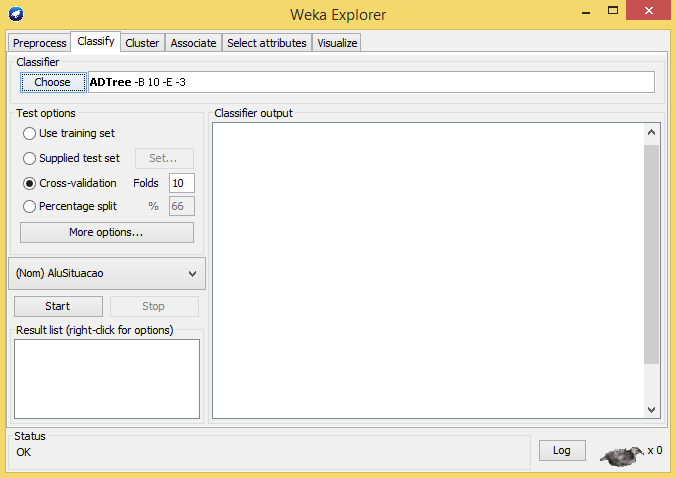
\includegraphics[width=11cm, height=8cm]{images/classificador}}
   	\caption {Tela de acesso aos algoritmos no Weka}
   	\label{classificador}
   \end{figure}
   
   \begin{figure}[!h]
   	\centering
   	{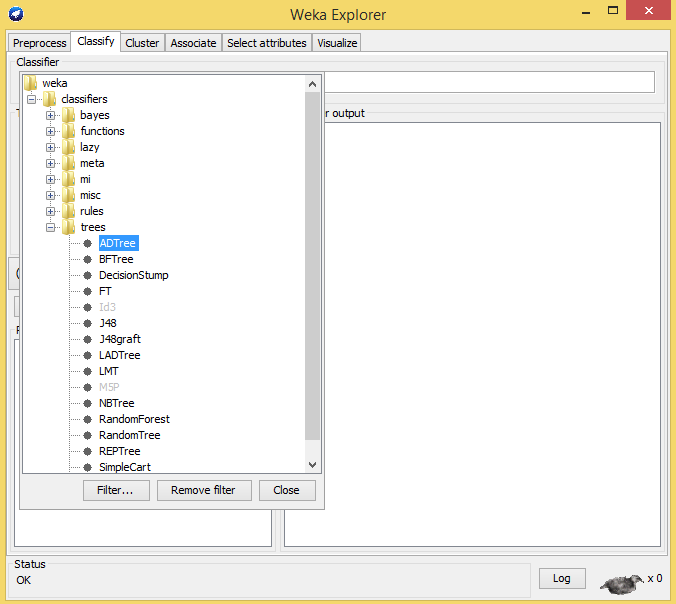
\includegraphics[width=10cm, height=8cm]{images/classificador2}}
   	\caption {Opções de algoritmos disponíveis no Weka}
   	\label{classificador2}
   \end{figure}

Entre as opções de teste, foi utilizada \textit{Cross-validation}, com o valor \textit{Folds} igual a 10. De acordo com \citet{witten2005}, o \textit{cross-validation} (ou \textit{validação cruzada}) realiza o processo de decisão sobre um número fixo de partições dos dados, onde dado um número de \textit{N} partições, são utilizadas \textit{N-1} partições para treinamento e o restante é utilizado para teste. A forma padrão de predizer uma técnica de aprendizagem dada uma amostra única e fixa de dados é utilizar a estratificação da validação cruzada 10 vezes, onde os dados são divididos aleatoriamente em 10 partes. Por padrão, o valor 10 é utilizado, onde 9 partições são utilizadas para treinamento e 1 para teste, porém o número de partições pode ser variável. As 10 estimativas de erros geradas pelas partições são calculadas para produzir uma estimativa de erro global.

O atributo escolhido para classificação foi o \textit{AluSituacao}, a partir do qual os algoritmos construíram regras para identificar a situação do aluno como \textit{cursando, formado} ou \textit{desligado}. Para cada arquivo ARFF analisado, foram identificados os algoritmos que geraram as melhores regras e conseguiram identificar o maior número de instâncias corretamente. A Figura \ref{weka5_mineracao} mostra os algoritmos previamente selecionados que apresentaram os melhores resultados para os dados de alunos ingressos no segundo semestre de 2005.

\begin{figure}[!h]
	\centering
	{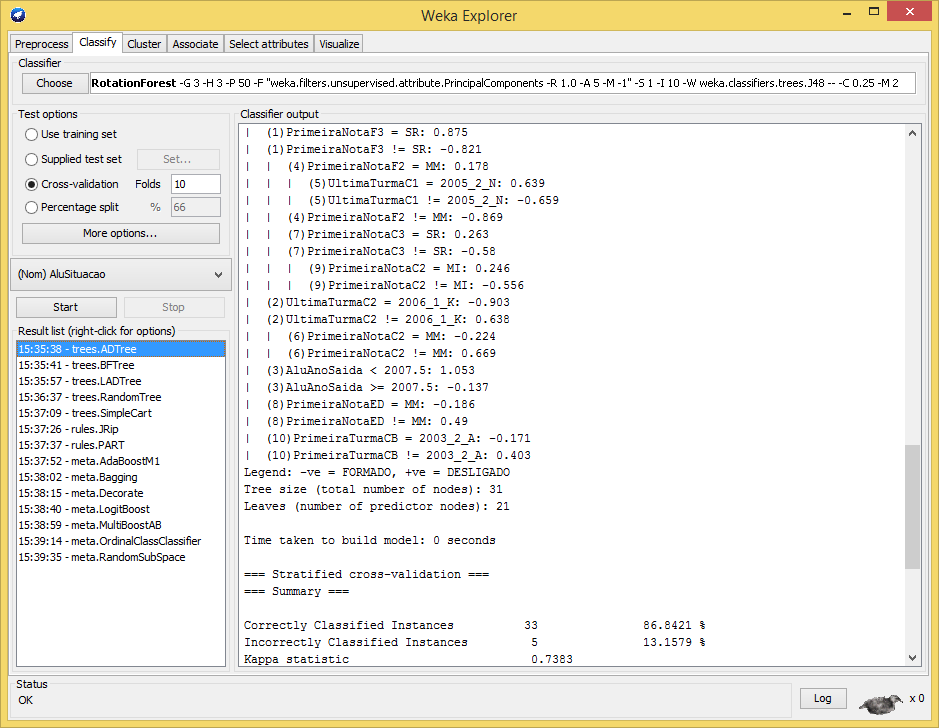
\includegraphics[width=11cm, height=10cm]{images/weka_mineracao}}
	\caption {Algoritmos selecionados para a análise dos dados de alunos ingressos no segundo semestre de 2005}
	\label{weka5_mineracao}
\end{figure}



 
  
\chapter{Resultados} \label{chapter6}

Este Capítulo apresenta os resultados obtidos por meio de consultas SQL e do processo de mineração de dados, seguindo a metodologia apresentada no Capítulo \ref{chapter5}. A Seção \ref{sec61} apresenta os resultados observados para os alunos por meio de consultas ao banco de dados, e a Seção \ref{sec62} apresenta os resultados obtidos para a evasão por meio do processo de mineração de dados realizado no Weka.

\section{Resultados Obtidos por Consultas SQL ao Banco de Dados} \label{sec61}

Os gráficos e resultados apresentados nesta Seção foram elaborados tomando por base consultas SQL realizadas no banco de dados. Foram selecionados os alunos para os quais foram verificados registros acadêmicos na tabela \textit{Histórico} a partir do primeiro semestre de curso, entre o ano de 2000 e 2013, o que indica que o aluno comprovadamente cursou uma ou mais das disciplinas analisadas durante os três primeiros semestres de curso. Ao todo, foram contabilizados 1.105 registros.

\subsection{Visão Geral} \label{visao_geral}
Dos 1.105 alunos identificados na base de dados que ingressaram no curso de Ciência da Computação da Universidade de Brasília entre 2000 e 2013, foram identificados 33,6\% dos alunos como formados, 36,9\% como desligados e 29,5\%  como cursando em 2014, conforme a Figura \ref{grafico9}. Ao verificar os percentuais obtidos por análise estatística dos dados, percebe-se que o índice de formatura entre o ano de 2000 e 2013 é menor se comparado ao índice de desligamento.

\begin{figure}[!h]
	\centering
	{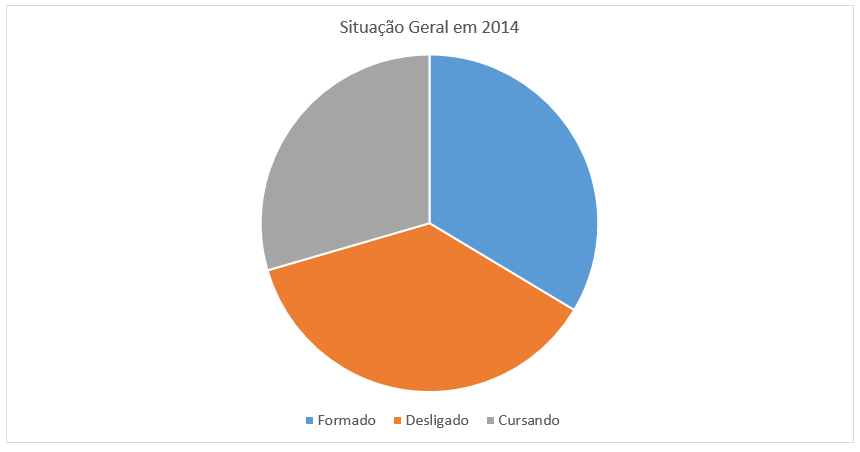
\includegraphics[width=14cm, height=7cm]{images/grafico9}}
	\caption {Situação dos alunos ingressantes entre 2000 e 2013 no ano de 2014.}
	\label{grafico9}
\end{figure}
  
Pela Figura \ref{grafico1}, a linha de tendência gerada pelo Excel aponta para o crescimento da quantidade de alunos ingressantes no curso de Ciência da Computação para os próximos semestres a partir de 2013. Entre o ano de 2000 e 2013, o número de alunos ingressantes variou entre 30 e 52 alunos por semestre.

\begin{figure}[!h]
	\centering
	{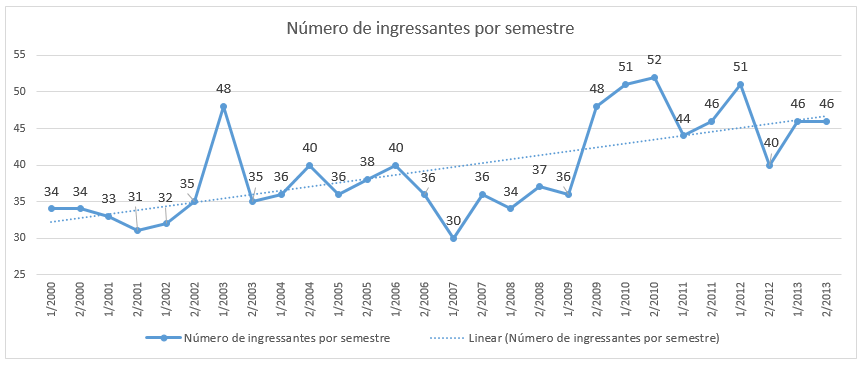
\includegraphics[width=16cm, height=6cm]{images/grafico1}}
	\caption {Gráfico de Ingressantes por Semestre no curso de Ciência da Computação da Universidade de Brasília entre o ano de 2000 e 2013.}
	\label{grafico1}
\end{figure}
  

A Figura \ref{grafico2} mostra o quantitativo de ingressantes, formados e desligados por semestre entre o ano de 2000 e 2013. O gráfico representa a situação dos alunos ingressantes por semestre no ano de 2014, período no qual os dados analisados foram obtidos. Tomando como exemplo os alunos que ingressaram no primeiro semestre de 2004, em 2014 não havia alunos na situação de cursando, 15 alunos foram constatados como desligados e 25 formados. Considerando que o aluno conclua o curso, em média, entre 10 e 12 semestres, justifica-se o crescimento da quantidade de alunos cursando e o decrescimento da quantidade de alunos formados a partir do ano de 2008. Anterior ao ano de 2008, o primeiro semestre de 2003 apresentou a maior quantidade de alunos que concluíram a graduação, somando 28 alunos formados. Se comparada a quantidade de formados pela quantidade de ingressantes por semestre, o segundo semestre de 2001 apresentou o melhor aproveitamento de alunos, com 80,6\% dos alunos de formados. Em contrapartida, o primeiro semestre de 2004 e o primeiro semestre de 2006 apresentaram a maior quantidade de alunos que não concluíram a graduação, somando 22 alunos desligados cada. Se comparada a quantidade de desligados pela quantidade de alunos ingressantes por semestre, o primeiro semestre de 2004 apresentou o pior aproveitamento de alunos, pois 61,1\% dos alunos ingressos saíram do curso antes do término. Cada coluna no gráfico representa a quantidade de alunos que foram identificados como cursando, formados ou desligados no ano de 2014.


\begin{figure}[!h]
	\centering
	{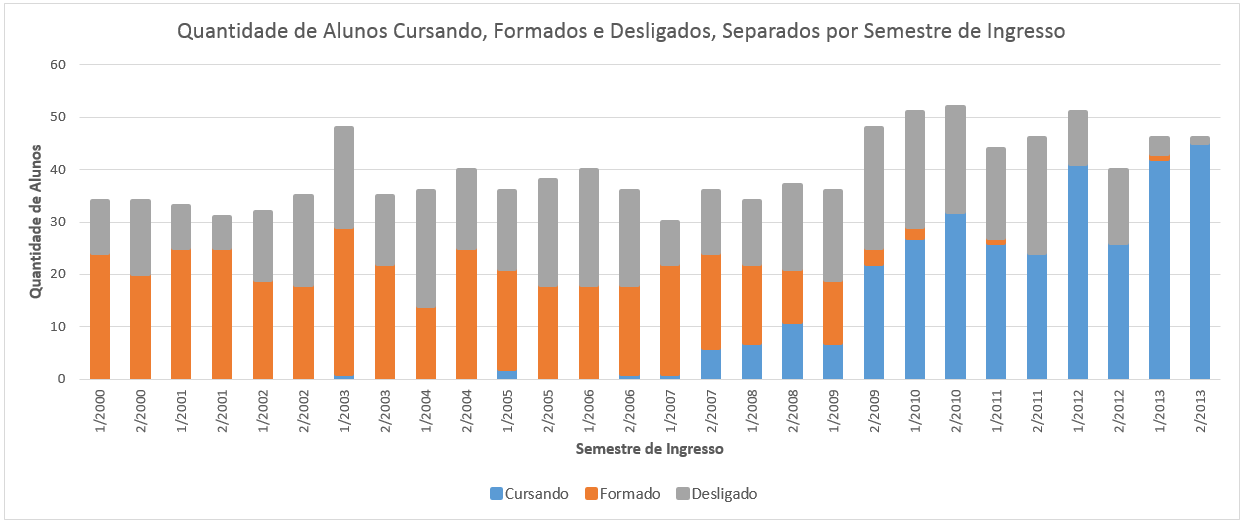
\includegraphics[width=16cm, height=5cm]{images/grafico2}}
	\caption {Situação dos alunos ingressantes por semestre no curso de Ciência da Computação da Universidade de Brasília no ano de 2014.}
	\label{grafico2}
\end{figure}


A Figura \ref{grafico10} apresenta as formas de ingresso para os alunos ingressantes entre 2000 e 2013, dada a situação do aluno em 2014. Dentre os alunos formados, 68,2\% ingressaram pelo vestibular, 26,1\% pelo Programa de Avaliação Seriada, 5,1\% por transferência obrigatória  e 0,6\% ingressaram por acordo cultural.

\begin{figure}[!htb]
	\centering
	{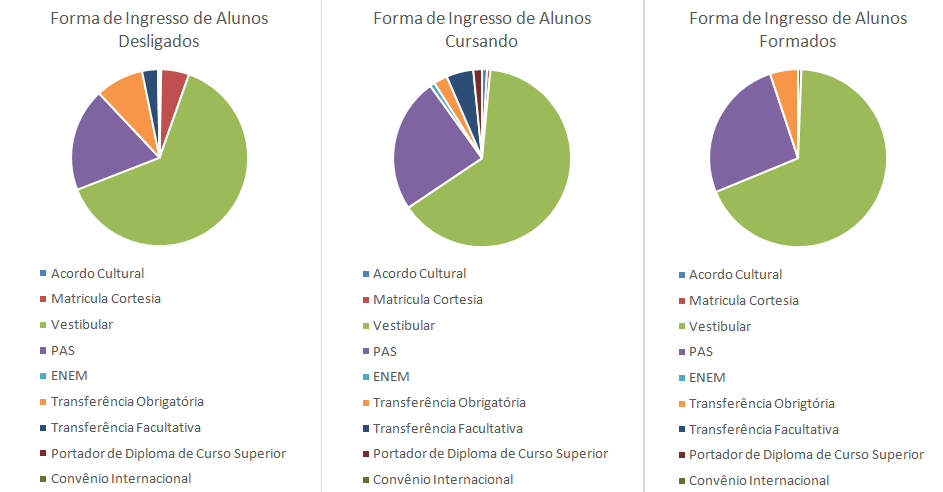
\includegraphics[width=14cm, height=7cm]{images/grafico10}}
	\caption {Formas de ingresso para os alunos identificados como formados, desligados e cursando em 2014.}
	\label{grafico10}
\end{figure}

Entre os alunos identificados como cursando, 64,1\% ingressaram pelo vestibular, 24,5\% pelo PAS, 4,9\% por transferência facultativa, 2,5\% por transferência obrigatória, 1,6\% por ser portador de diploma de curso superior e 0,9\% pelo Exame Nacional do Ensino Médio (ENEM).

Dentre os alunos identificados como desligados, 63,7\% ingressaram pelo vestibular, 18,9\% pelo PAS, 8,8\% por transferência obrigatória, 5,1\% por matricula cortesia, 2,9\% por transferência facultativa, 0,3\% por convênio internacional e 0,3\% por acordo cultural. Do gráfico, percebe-se que entre 2000 e 2013 não houve registros de formados por alunos ingressos por matrícula cortesia, ENEM, transferência facultativa, por ser portador de diploma de curso superior e convênio internacional.
 
 Analisando os motivos de evasão por semestre, percebe-se que os motivos mais recorrentes para justificar a evasão dos alunos em geral foram o desligamento por abandono, por não cumprimento de condição, desligamento voluntário, desligamento por reprovar três vezes a mesma disciplina obrigatória, por novo vestibular e por transferência. Do mesmo modo, pode-se constatar que o desligamento por falecimento e por decisão judicial são eventuais, ocorrendo em menor frequência ao longo dos anos. Dos alunos desligados entre 2000 e 2013, apenas 0,2\% foram desligados por falecimento e 0,7\% por decisão judicial. A Tabela \ref{desligamento_geral} detalha o percentual de alunos ingressantes por semestre, entre o ano de 2000 e 2013, que foram identificados como desligados em 2014, separados por motivo de desligamento. Foram considerados para a tabela apenas os motivos mais recorrentes de desligamento identificados na base de dados.
 
 \begin{longtable}{C{1,8cm}|C{1,9cm}C{2,0cm}C{1,9cm}C{2,1cm}C{2cm}C{2,0cm}}
 	\caption{Percentual de alunos desligados por motivo.} 	\label{desligamento_geral} \\
 	\hline
 	Semestre & \multicolumn{6}{|c}{Percentual (\%) de Desligamento por Motivo}\\ 
 	\hline
 	& Abandono & Não Cumpriu Condição & Voluntário & Reprovou 3 vezes Mesma Disciplina Obr. & Novo Vestibular & Transferência\\
 	\hline
 	1/2000 & 10 & 60 & 30 & 0 & 0 & 0\\
 	2/2000 & 28,6 & 50 & 14,3 & 0 & 0 & 7,1\\
 	1/2001 & 12,5 & 75 & 12,5 & 0 & 0 & 0\\
 	2/2001 & 33,3 & 16,7 & 50 & 0 & 0 & 0\\
 	1/2002 & 0 & 46,1 &  38,5 & 0 & 7,7 & 7,7\\
 	2/2002 & 0 & 46,1 & 38,5 & 0 & 7,7 & 7,7\\
 	1/2003 & 21,05 & 47,4 & 10,5 & 21,05 & 0 & 0\\
 	2/2003 & 23 & 38,5 & 15,4 & 7,7 & 7,7 & 7,7\\
 	1/2004 & 27,3 & 27,3 & 36,4 & 0 & 0 & 4,5\\
 	2/2004 & 6,7 & 46,7 & 26,7 & 0 & 0 & 0\\
 	1/2005 & 40 & 26,7 & 20 & 13,3 & 0 & 0\\
 	2/2005 & 20 & 60 & 5 & 0 & 10 & 5\\
 	1/2006 & 18,2 & 45,5 & 4,6 & 0 & 9 & 22,7\\
 	2/2006 & 11,1 & 38,9 & 27,8 & 11,1 & 11,1 & 0\\
 	1/2007 & 12,5 & 37,5 & 37,5 & 0 & 0 & 12,5\\
 	2/2007 & 33,3 & 58,3 & 0 & 8,4 & 0 & 0\\
 	1/2008 & 8,3 & 41,7 & 17,7 & 0 & 33,3 & 0\\
 	2/2008 & 6,25 & 37,5 & 25 & 25 & 0 & 6,25\\
 	1/2009 & 5,9 & 23,5 & 29,4 & 17,6 & 23,5 & 0\\
 	2/2009 & 4,35 & 26,1 & 8,7 & 17,4 & 39,1 & 4,35\\
 	1/2010 & 13,6 & 36,4 & 4,6 & 0 & 31,8 & 13,6\\
 	2/2010 & 15 & 55 & 0 & 10 & 20 & 0\\
 	1/2011 & 5,9 & 52,9 & 5,9 & 35,3 & 0 & 0\\
 	2/2011 & 0 & 77,3 & 0 & 9,1 & 9,1 & 4,5\\
 	1/2012 & 10 & 70 & 0 & 0 & 20 & 0\\
 	2/2012 & 0 & 78,6 & 0 & 7,1 & 14,3 & 0\\
 	1/2013 & 0 & 33,3 & 33,3 & 0 & 33,3 & 0\\
 	\hline
 \end{longtable} 

\subsection{Análise dos Alunos por Gênero} \label{analise_genero}

A Figura \ref{grafico3} mostra a quantidade de alunas ingressantes por semestre entre 2000 e 2013, e a quantidade das mesmas que foram identificadas como formadas no ano de 2014. Pelo gráfico, o primeiro semestre de 2005 e o primeiro semestre de 2010 registraram a maior quantidade de alunas ingressantes, totalizando 10 alunas cada. Se comparada a quantidade de alunas formadas sobre o total de alunas ingressantes por semestre, o primeiro semestre de 2001 apresentou o melhor aproveitamento das alunas, pois 100\% das alunas ingressantes formaram-se, seguido do primeiro semestre de 2003, com aproveitamento de 86\% de alunas formadas. 
  
\begin{figure}[!h]
	\centering
	{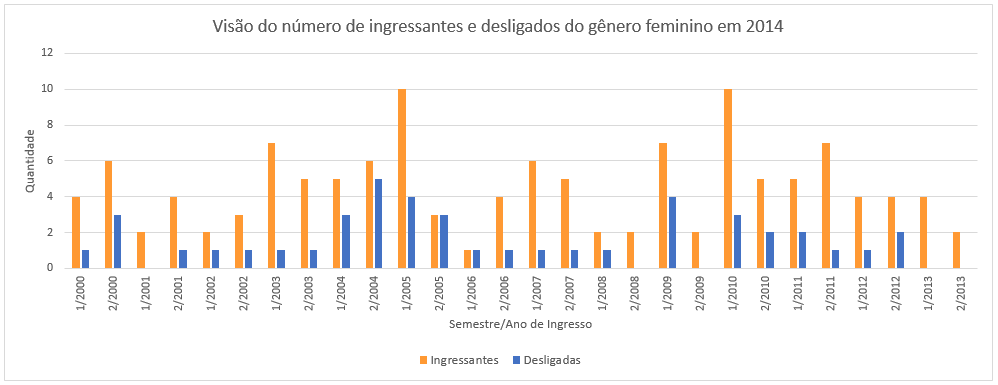
\includegraphics[width=16cm, height=6cm]{images/grafico3}}
	\caption {Quantidade de alunas ingressantes por semestre  entre o ano de 2000 e 2013 e quantidade de alunas que foram identificadas como formadas no curso de Ciência da Computação da Universidade de Brasília no ano de 2014.}
	\label{grafico3}
\end{figure}

A Figura \ref{grafico4} mostra a quantidade de alunos do sexo masculino ingressantes por semestre entre 2000 e 2013, e a quantidade dos mesmos que foram identificados como formados no ano de 2014. Ao comparar o número de alunos ingressantes e formados por gênero, percebe-se que há uma predominância dos alunos do sexo masculino no curso de Ciência da Computação da Universidade de Brasília. Se comparada a quantidade de alunos formados sobre o total de alunos ingressantes do sexo masculino, o segundo semestre de 2001 e o primeiro semestre de 2001 apresentaram o melhor aproveitamento de alunos, pois formaram 81\% e 74\% dos alunos ingressantes, respectivamente. 

\begin{figure}[!h]
	\centering
	{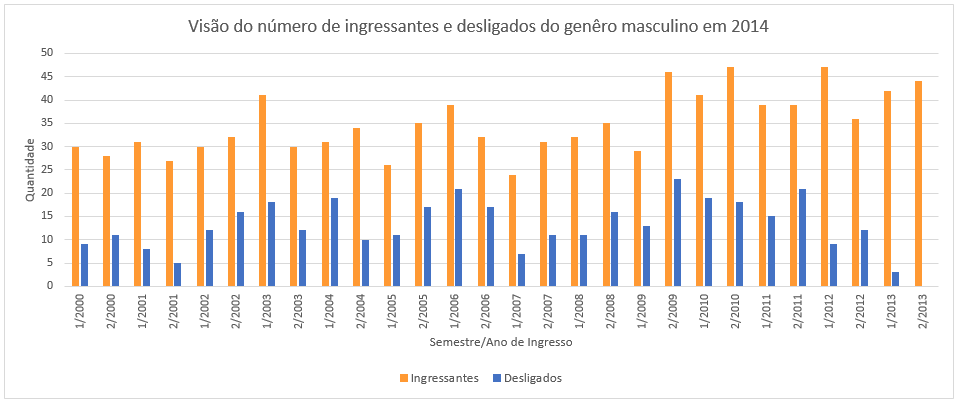
\includegraphics[width=16cm, height=6cm]{images/grafico4}}
	\caption {Quantidade de alunos do sexo masculino ingressantes por semestre  entre o ano de 2000 e 2013 e quantidade de alunos que foram identificados como formados no curso de Ciência da Computação da Universidade de Brasília no ano de 2014.}
	\label{grafico4}
\end{figure}

A Figura \ref{grafico7} apresenta a visão do percentual de desligamento geral em 2014, separado por semestre. Do total de alunos que ingressaram no primeiro semestre de 2004 e no primeiro semestre de 2006, 61,1\% e 55\%, respectivamente, foram identificados como desligados em 2014, sendo estes considerados os semestres com maior percentual de evasão entre 2000 e 2013.

\begin{figure}[!h]
	\centering
	{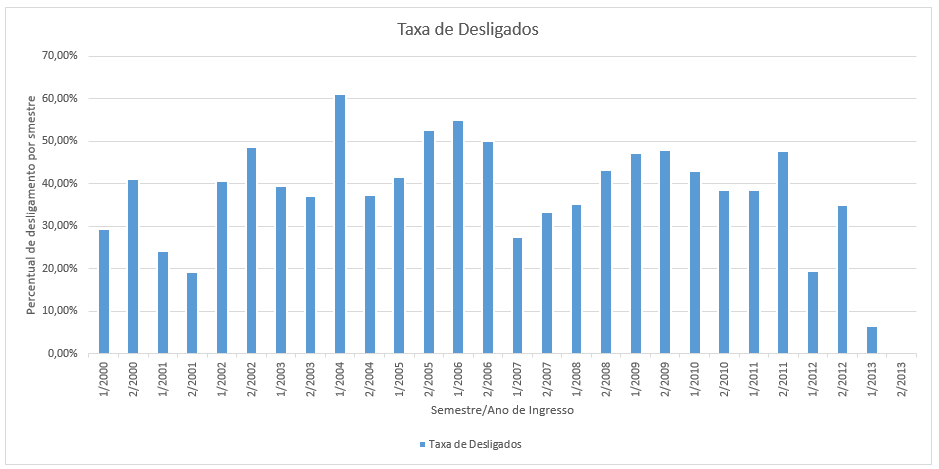
\includegraphics[width=16cm, height=6cm]{images/grafico7}}
	\caption {Visão da taxa de desligamento geral por semestre no ano de 2014.}
	\label{grafico7}
\end{figure}


As Figuras \ref{grafico5} e \ref{grafico6} mostram o comparativo de alunos que foram identificados como formados e desligados no ano de 2014, separados por gênero. Entre 2000 e 2008, percebe-se a maior variação da taxa de alunos formados e desligados para o gênero feminino, tendo sido constatados semestres com 100\% de aproveitamento (primeiro semestre de 2001) e com 0\% de aproveitamento (segundo semestre de 2005 e primeiro semestre de 2006) das alunas ingressantes. Para o gênero masculino, a taxa de formados por semestre variou entre 38,1\% (primeiro semestre de 2004) e 81,5\% (segundo semestre de 2001). 

\begin{figure}[!h]
	\centering
	{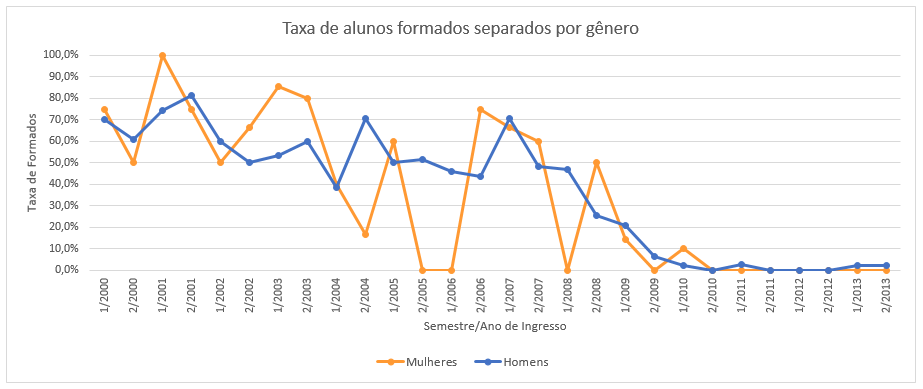
\includegraphics[width=16cm, height=6cm]{images/grafico5}}
	\caption {Taxa de alunos formados por semestre entre o ano de 2000 e 2013 separados por gênero.}
	\label{grafico5}
\end{figure}

\begin{figure}[!h]
	\centering
	{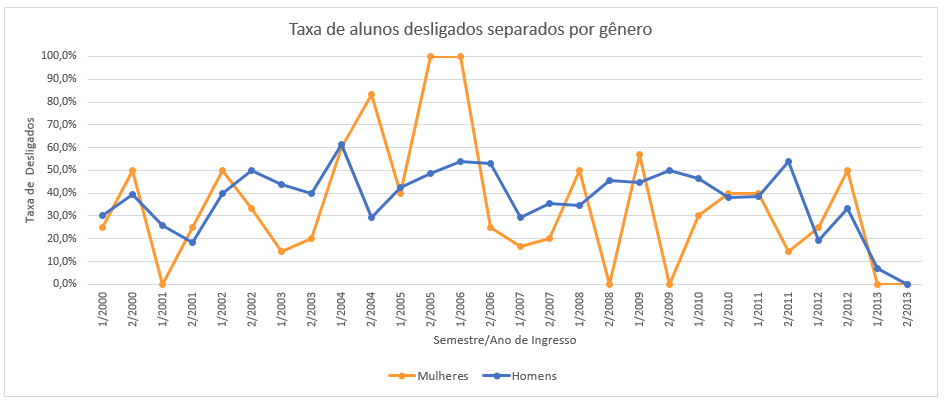
\includegraphics[width=16cm, height=6cm]{images/grafico6}}
	\caption {Taxa de alunos desligados por semestre entre o ano de 2000 e 2013 separados por gênero.}
	\label{grafico6}
\end{figure}


A Figura \ref{grafico8} apresenta as formas de saída observadas para os alunos que foram identificados como desligados em 2014. Dos alunos ingressantes entre 2000 e 2013, 46,6\% foram desligados por não cumprimento de condição, 14,2\% por abandono, 14,2\% por desligamento voluntário, 11,8\% por novo vestibular, 10,3\% por reprovar três vezes a mesma disciplina obrigatória, 2\% por transferência, 0,7\% por decisão judicial e 0,2\% por falecimento.

\begin{figure}[!h]
	\centering
	{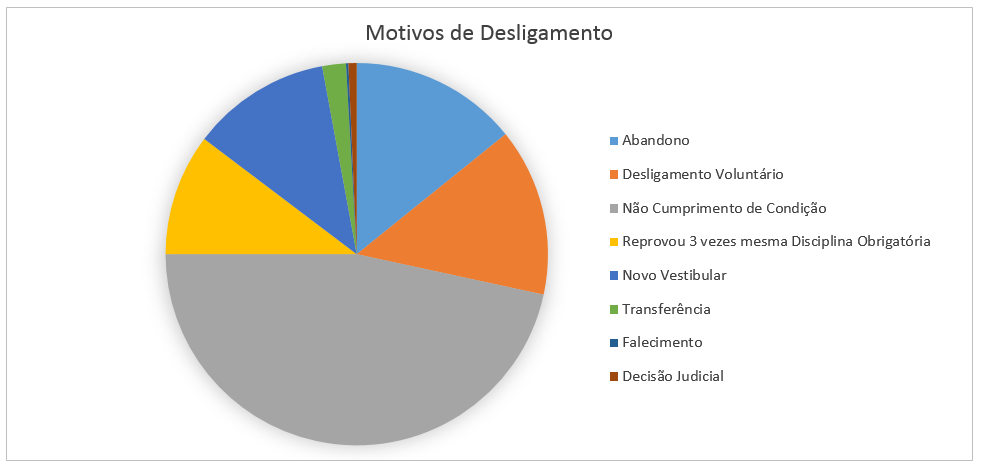
\includegraphics[width=13cm, height=6cm]{images/grafico8}}
	\caption {Formas de desligamento identificadas para os alunos em geral ingressos entre 2000 e 2013.}
	\label{grafico8}
\end{figure}
 

A partir dos dados gerais obtidos entre 2000 e 2013 e analisando-os por gênero dos alunos, pode-se constatar que:
\begin{itemize}
	\item Entre o ano de 2000 e 2013, foram contabilizadas 127 alunas que matricularam-se no curso de Ciência da Computação. Deste total, no ano de 2014 haviam 34,7\% alunas desligadas, 36,2\% formadas e  29,1\% cursando. No mesmo período, foram contabilizados 978 alunos do sexo masculino no curso de Ciência da Computação. Deste total, no ano de 2014, haviam 37,2\% alunos desligados, 33,3\% formados e 29,5\% cursando;
	
	\item Dentre as alunas formadas, 76\% não informaram a escola de origem onde cursaram o Ensino Médio. Em relação aos alunos formados, esse percentual aumenta para 78,5\%;
	
	\item 97,1\% das alunas formadas ingressaram na UnB pelo sistema universal e 2,9\% pelo sistema de cotas para negros.  Dos alunos formados, 95,1\% ingressaram pelo sistema universal e 4,9\% por sistemas de cotas para negros;
	
	\item Das alunas formadas que informaram a escola de origem onde concluíram o Ensino Médio, 90,9\% são oriundas de escola particular e 9,1\% de escola pública.  Dentre os alunos formados que informaram a escola de origem, 84,3\% cursaram o Ensino Médio em escola particular e 25,7\% em escola pública;
	
	\item Das alunas formadas que cursaram o Ensino Médio em escola particular, 80\% foram aprovadas pelo sistema universal e 20\% pelo sistema de cotas para negros. Entre as alunas formadas que cursaram o Ensino Médio em escola pública, 100\% foram aprovadas pelo sistema universal. Para os alunos formados que cursaram o Ensino Médio em escola particular, 93,2\% foram aprovados pelo sistema universal e 6,8\% pelo sistema de cotas para negros. Entre os alunos formados que cursaram o Ensino Médio em escola pública, 91\% foram aprovados pelo sistema universal e 9\% pelo sistema de cotas para negros;
	
	\item As alunas formadas ingressaram no curso na faixa etária dos 16 aos 32 anos, sendo que 76\% ingressou no curso com idade entre 17 e 19 anos.  Os alunos formados ingressaram no curso na faixa etária dos 16 a 35 anos, e destes, 73,5\% ingressaram com idade entre 17 e 19;
	
	\item Das alunas formadas, 60,9\% ingressaram pelo vestibular, 26\% pelo Programa de Avaliação Seriada (PAS), 10,9\% por transferência obrigatória e 2,2\% por acordo cultural;
	
	\item Dos alunos formados, 29,8\% formaram-se antes do 10º semestre, 55,1\% entre o 10º e 12º semestre, e 15,1\% após o 12º semestre; 
	
	\item As alunas formadas levaram em média 11 semestres para concluir o curso, e os alunos em média 10 semestres;
	
	\item As alunas desligadas cursaram, em média, 5 semestres. Para os alunos desligados, a média aumenta para 6 semestres;
	
	\item Das alunas desligadas, 68\% ingressaram na faixa etária entre 17 e 19 anos;
	
	\item 70\% das alunas desligadas não informaram em qual tipo de escola (pública ou particular) cursaram o Ensino Médio. Para os alunos, esse percentual é reduzido para 64,3\%;
	
	\item Das alunas desligadas que informaram a escola de origem na qual cursaram o Ensino Médio, 84\% são oriundas de escola particular, e entre os alunos, 70,8\% são oriundos de escola particular;
	
	\item Todas as alunas desligadas que cursaram o Ensino Médio em escola pública ou particular foram aprovadas pelo sistema universal. Dos alunos desligados que cursaram o Ensino Médio em escola particular, 87\% foram aprovados pelo sistema universal e  13\% pelo sistema de cotas para negros. Dos alunos desligados que cursaram o Ensino Médio em escola pública, 5,3\% foram aprovados pelo sistema de cotas para escola pública de alta renda PPI, 28,9\% pelo sistema de cotas para negros e 65,8\% pelo sistema universal; 
	
	\item 97,7\% das alunas desligadas foram aprovadas pelo sistema universal e 2,3\% pelo sistema de cotas para negros. Dos alunos desligados, 87,4\% foram aprovados pelo sistema universal, 12,1\% pelo sistema de cotas para negros e 0,5\% por cotas para escola pública de alta renda PPI;
	
	\item Entre as alunas desligadas, 47,7\% ingressaram pelo vestibular, 22,5\% pelo Programa de Avaliação Seriada (PAS), 15,9\% por transferência obrigatória e 13,6\% por matrícula cortesia. Entre os alunos desligados, 0,3\% ingressaram por acordo cultural, 0,3\% por convênio internacional, 4,1\% por matrícula cortesia, 18,4\% pelo Programa de Avaliação Seriada (PAS), 3,3\% por transferência facultativa, 8\% por transferência obrigatória e 65,6\% pelo vestibular;
	
	
	\item Dos alunos desligados que cursaram o Ensino Médio em escola particular, 87\% foram aprovados pelo sistema universal e  13\% pelo sistema de cotas para negros. Dos alunos desligados que cursaram o Ensino Médio em escola pública, 5,3\% foram aprovados pelo sistema de cotas para escola pública de alta renda PPI, 28,9\% pelo sistema de cotas para negros e 65,8\% pelo sistema universal; 
	
	\item Entre todas as alunas desligadas, 22,7\% foi por abandono, 6,8\% por decisão judicial, 22,7\% por não cumprimento de condição, 25\% por desligamento voluntário, 18,2\% por novo vestibular, 2,3\% por reprovar três vezes a mesma disciplina obrigatória e 2,3\% por transferência. 	Entre todos os alunos desligados, 13,2\% foi por abandono, 49,4\% por não cumprimento de condição, 12,9\% por desligamento voluntário, 0,3\% por falecimento, 11\% por novo vestibular, 11,3\% por reprovar três vezes a mesma disciplina obrigatória e 1,9\% por transferência;
	
	\item 56,8\% das alunas desligadas saíram do curso entre o 1º e o 3º semestre, 18,2\% saíram entre o 4º e o 7º semestre e 25\% saíram após o 7º semestre do curso. Analisando o mesmo cenário para os alunos desligados, 36\% saíram entre o 1º e o 3º semestre, 41,2\% entre o 4º e o 7º semestre e 22,8\% após o 7º semestre;
	
	\item Das alunas desligadas entre o 1º e o 3º semestre do curso, 12\% foi por abandono, 12\% por decisão judicial, 28\% por desligamento voluntário, 20\% por não cumprimento de condição, 24\% por novo vestibular e 4\% por transferência. Dos alunos desligados no mesmo período, 6,1\% saíram por motivo de abandono,  53,4\% por não cumprimento de condição, 16,8\% por desligamento voluntário, 9,2\% por novo vestibular, 11,4\% por reprovar três vezes a mesma disciplina obrigatória e 3\% por transferência;
	
	\item Das alunas desligadas entre o 4º e o 7º semestre do curso, 12,5\% foi por abandono, 37,5\% por não cumprimento de condição, 25\% por desligamento voluntário, 12,5\% por novo vestibular e 12,5\% por reprovar três vezes a mesma disciplina obrigatória.  Dos alunos desligados no mesmo período, 12,8\% saíram por motivo de abandono, 50\% por não cumprimento de condição, 11,3\% por desligamento voluntário, 15,3\% por novo vestibular, 9,3\% por reprovar três vezes a mesma disciplina obrigatória e 1,3\% por transferência; 
	
	\item Das alunas desligadas após o 7º semestre do curso, 54,5\% foi por motivo de abandono, 18,2\%  por não cumprimento de condição, 18,2\% por desligamento voluntário e 0,1\% por novo vestibular. Dos alunos desligados após o 7º semestre, 25,3\% saíram por motivo de abandono, 42,2\% por não cumprimento de condição, 9,6\% por desligamento voluntário, 1,2\% por falecimento, 6\% por novo vestibular, 14,5\% por reprovar três vezes a mesma disciplina obrigatória e 1,2\% por transferência.
\end{itemize}

\subsection{Análise das Disciplinas}

A partir da análise dos dados armazenados nas tabelas \textit{evasao\_cic, evasao\_mat} e \textit{evasao\_cic}, constatou-se que:
\begin{itemize} 
	\item Dos alunos em geral que cursaram a disciplina Computação Básica, 17,35\% não cursaram a disciplina Estruturas de Dados e 31,85\% não cursaram a disciplina Programação Sistemática. Considerando apenas os alunos desligados que cursaram a disciplina Computação Básica, 31,12\% não cursaram a disciplina Estruturas de Dados e 55,63\% não cursaram a disciplina Programação Sistemática;
	\item Dos alunos em geral que cursaram a disciplina Cálculo 1, 25,21\% não cursaram a disciplina Cálculo 2 e 38,65\% não cursaram a disciplina Cálculo 3. Considerando apenas os alunos desligados que cursaram a disciplina Cálculo 1, 36,31\% não cursaram a disciplina Cálculo 2 e 60,83\% não cursaram a disciplina Cálculo 3;
	\item Dos alunos em geral que cursaram a disciplina Física 1, 28,90\% não cursaram a disciplina Física 2 e 42,18\% não cursaram a disciplina Física 3. Considerando apenas os alunos desligados que cursaram a disciplina Física 1, 48,71\% não cursaram a disciplina Física 2 e 68,46\% não cursaram a disciplina Física 3.
\end{itemize}

A Figura \ref{taxa_reprovados} mostra a taxa de reprovação geral entre 2000 e 2013 para as disciplinas ofertadas nos três primeiros semestres do curso . Analisando as taxas de reprovação por departamento, as disciplinas observadas com maiores índices de reprovação foram Computação Básica (26,06\%), Cálculo 3 (45,2\%) e Física 1 (37,13\%). Analisando todas as disciplinas apresentadas no gráfico, a disciplina Cálculo 3 apresenta a maior taxa de reprovação, seguida de Cálculo 1 (38,09\%) e Física 1 (37,13\%).

\begin{figure}[!h]
	\centering
	{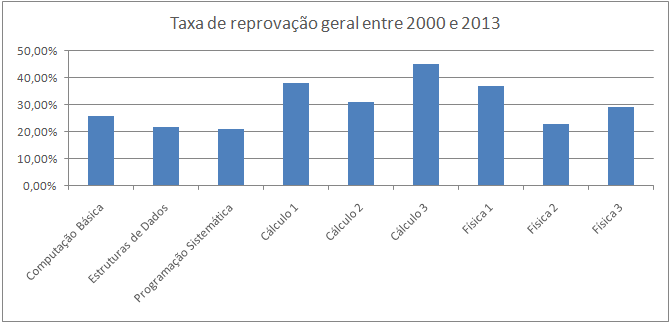
\includegraphics[width=13cm, height=6cm]{images/taxa_reprovados}}
	\caption {Taxa de reprovação geral entre 2000 e 2013 para as disciplinas obrigatórias ofertadas nos três primeiros semestres.}
	\label{taxa_reprovados}
\end{figure}

Ao analisar a taxa de desligamento por disciplina considerando apenas os dados dos alunos identificados como desligados, constatou-se que o índice de reprovação é superior se comparado aos índices de reprovação geral, conforme mostrado na Figura \ref{reprovados_desligados}. Para todas as disciplinas analisadas, com exceção da disciplina Estruturas de Dados, foram verificadas taxas de reprovação acima de 50\%. Analisando por departamento, as disciplinas observadas com maiores índices de reprovação para os alunos desligados foram Programação Sistemática (53,59\%), Cálculo 3 (80,69\%) e Física 3 (73,17\%). Analisando todas as disciplinas apresentadas no gráfico, a disciplina Cálculo 3 apresentou a maior taxa de reprovação, seguida de Física 3 e Cálculo 1 (70,84\%).

\begin{figure}[!h]
	\centering
	{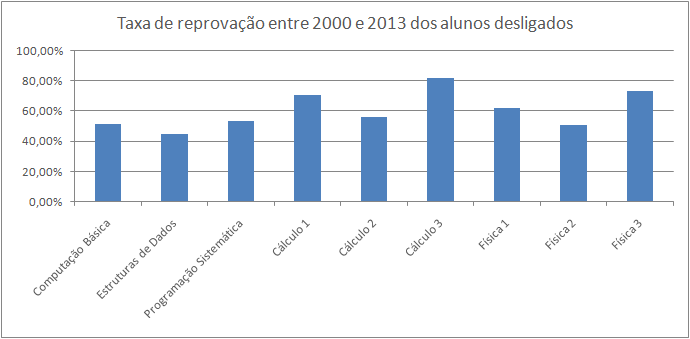
\includegraphics[width=13cm, height=6cm]{images/reprovados_desligados}}
	\caption {Taxa de reprovação entre 2000 e 2013 dos alunos desligados para as disciplinas obrigatórias ofertadas nos três primeiros semestres.}
	\label{reprovados_desligados}
\end{figure}

A Figura \ref{reprova3} apresenta o percentual geral de alunos que reprovaram três vezes a mesma disciplina para os três primeiros semestres. Para a disciplina Programação Sistemática, não foram identificados alunos que reprovaram ao cursar pela terceira vez. Para as demais disciplinas, foi identificada uma variação entre 0,76\% (Cálculo 3) e 3,64\% (Física 1). Analisando por departamento, as disciplinas observadas com maiores índices de reprovação ao serem cursadas pela terceira vez foram Computação Básica (2,44\%), Cálculo 1 (2,05\%) e Física 1 (3,64\%).

\begin{figure}[!h]
	\centering
	{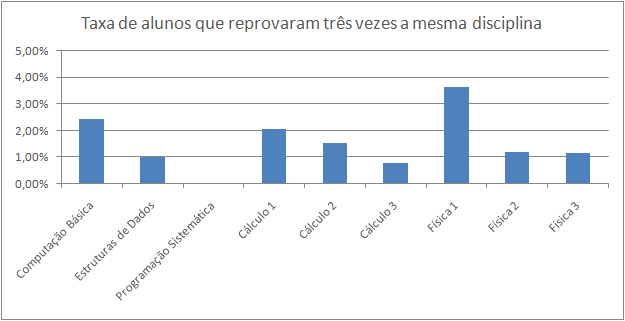
\includegraphics[width=13cm, height=6cm]{images/reprova3}}
	\caption {Percentual de alunos que reprovaram três vezes a mesma disciplina obrigatória.}
	\label{reprova3}
\end{figure}

As Tabelas \ref{mencao_geral} e \ref{mencao_desligados} apresentam, respectivamente, o percentual de menções obtidas pelos alunos em geral e pelos alunos desligados nas disciplinas obrigatórias dos três primeiros semestres. Foram consideradas para o cálculo dos percentuais apenas as primeiras menções obtidas pelos alunos ao cursaram as disciplinas. 

Das menções obtidas pelos alunos em geral, foi identificado que nas disciplinas ofertadas pelo Departamento de Matemática (MAT-UnB), o percentual de menções SR, II e MI é maior se comparadas as demais disciplinas apresentadas. Para as disciplinas ofertadas pelo Instituto de Física (IF-UnB), foi verificado um maior percentual de menções MM, e para o Departamento de Ciência da Computação foi verificado um maior percentual de menções MS e SS nas disciplinas introdutórias. 

Para todas as disciplinas apresentadas na Tabela \ref{mencao_geral}, as menções TR e TJ varia entre 0\% e 6,1\%. Analisando os maiores percentuais por menção, verifica-se que:
\begin{itemize}
	\item O maior percentual de menção TR foi verificado em Cálculo 3, com 6,1\%;
	\item O maior percentual de menção TJ foi verificado em Física 1, com 1\%;
	\item O maior percentual de menção SR foi verificado em Cálculo 3, com 11\%;
	\item O maior percentual de menção II foi verificado em Física 1, com 16\%;
	\item O maior percentual de menção MI foi verificado em Cálculo 3, com 13,7\%;
	\item O maior percentual de menção MM foi verificado em Física 3, com 44,7\%;
	\item O maior percentual de menção MS foi verificado em Programação Sistemática, com 32,1\%;
	\item O maior percentual de menção SS foi verificado em Computação Básica, com 19,8\%.
	\end{itemize}

 \begin{longtable}{C{3,8cm}|C{0,9cm}C{0,9cm}C{0,9cm}C{0,9cm}C{0,9cm}C{0,9cm}C{0,9cm}C{0,9cm}C{0,9cm}}
 	\caption{Percentual de menções por disciplina dos alunos em geral.} 	\label{mencao_geral}\\
 	\hline
 	\multicolumn{1}{c}{Disciplina} & \multicolumn{9}{|c}{Percentual (\%) de Menções}\\ 
 	\hline
 	 & TR & TJ & SR & II & MI & MM & MS & SS & CC\\ \hline
 	Computação Básica & 0,8 & 0,3 & 5,3 & 9,5 & 9,5 & 19,5 & 29,7 & 19,8 & 5,6\\ 
 	Estruturas de Dados & 1,5 & 0,1 & 5,5 & 7,4 & 6,7 & 26,3 & 29,4 & 19 & 4\\
 	Progr. Sistemática & 3,6 & 0,3 & 5,8 & 3,9 & 7,3 & 33,7 & 32,1 & 12,1 & 1,2\\ \hline
 	Cálculo 1 & 0,8 & 0,6 & 7,6 & 14,1 & 12,6 & 31 & 19,4 & 7,5 & 6,4\\
 	Cálculo 2 & 1,3 & 0,7 & 5,9 & 11,2 & 10,5 & 37,9 & 21,8 & 8,8 & 1,9\\
 	Cálculo 3 & 6,1 & 0,3 & 11 & 13,1 & 13,7 & 36,4 & 15,5 & 2,7 & 1,2\\ \hline
 	Física 1 & 1,5 & 1 & 6,1 & 16 & 10,8 & 32,5 & 19,9 & 9,8 & 2,4\\
 	Física 2 & 2 & 0,1 & 5,5 & 4,9 & 9,9 & 43 & 26,7 & 6,7 & 1,2\\
 	Física 3 & 1,8 & 1 & 7,8 & 7 & 11,2 & 44,7 & 17,6 & 7,4 & 1,6\\
 	\hline
  \end{longtable} 
 
 Das menções obtidas pelos alunos desligados, verificou-se que há uma diminuição no desempenho dos alunos desligados em todas as disciplinas, se comparadas com a média geral. Foi identificada uma diminuição nos percentuais de menções MM, MS e SS (menções de aprovação), e em contrapartida, um aumento no percentual de menções SR, II e MI (menções de reprovação). Tomando como exemplo a disciplina Física 3, percebe-se para os alunos desligados um aumento de 33\% na taxa de menções SR e uma diminuição de 11\% na taxa de menções SS, se comparados ao desempenho dos alunos em geral.
 
 Analisando os maiores percentuais por menção dos alunos desligados, verifica-se que:
 \begin{itemize}
 	\item O maior percentual de menção TR foi verificado em Cálculo 3, com 7,8\%;
 	\item O maior percentual de menção TJ foi verificado em Física 1 e Física, ambos com 0,8\%;
 	\item O maior percentual de menção SR foi verificado em Cálculo 3, com 28,8\%;
 	\item O maior percentual de menção II foi verificado em Cálculo 1, com 22,3\%;
 	\item O maior percentual de menção MI foi verificado em Computação Básica, com 16,2\%;
 	\item O maior percentual de menção MM foi verificado em Física 2, com 38,5\%;
 	\item O maior percentual de menção MS foi verificado em Computação Básica, com 21,1\%;
 	\item O maior percentual de menção SS foi verificado em Computação Básica, com 11,8\%.
 \end{itemize}
 
 \begin{longtable}{C{3,8cm}|C{0,9cm}C{0,9cm}C{0,9cm}C{0,9cm}C{0,9cm}C{0,9cm}C{0,9cm}C{0,9cm}C{0,9cm}}
 	\caption{Percentual de menções por disciplina dos alunos desligados.} 	\label{mencao_desligados}\\
 	\hline
 	\multicolumn{1}{c}{Disciplina} & \multicolumn{9}{|c}{Percentual (\%) de Menções}\\ 
 	\hline
 	& TR & TJ & SR & II & MI & MM & MS & SS & CC\\ \hline
 	Computação Básica & 1,7 & 0,2 & 9,8 & 14,5 & 16,2 & 17,6 & 21,1 & 11,8 & 7,1\\ 
 	Estruturas de Dados & 2,8 & 0 & 12,5 & 13,9 & 9,3 & 26 & 21 & 10 & 4,6\\
 	Progr. Sistemática & 3,9 & 0,6 & 16,6 & 8,8 & 11 & 37 & 14,9 & 3,9 & 3,3\\ \hline
 	Cálculo 1 & 2 & 0,3 & 14,8 & 22,3 & 13,3 & 25,3 & 11 & 3,1 & 7,9\\
 	Cálculo 2 & 0,4 & 0,8 & 13,3 & 16,1 & 15,7 & 32,9 & 12,9 & 4,8 & 3,2\\
 	Cálculo 3 & 7,8 & 0 & 28,8 & 18,3 & 11,1 & 20,9 & 10,5 & 0,7 & 2\\ \hline
 	Física 1 & 3,3 & 0,8 & 13,6 & 19,7 & 12,1 & 28,2 & 13,8 & 6,4 & 2,1\\
 	Física 2 & 0,5 & 0 & 13,5 & 9 & 16 & 38,5 & 18,5 & 3 & 1\\
 	Física 3 & 5,7 & 0,8 & 23,6 & 10,6 & 14,6 & 35 & 7,3 & 0,8 & 1,6\\
 	\hline
 \end{longtable}
 
\section{Resultados Obtidos por Mineração de Dados} \label{sec62}

Nas Seções \ref{resultado1} e \ref{resultado2} são apresentadas as regras e padrões descobertos pelo processo de mineração de dados. Primeiramente, foi realizado o processo de mineração sobre os 1.105 registros dos alunos que ingressaram no curso entre 2000 e 2013, apresentado na Seção \ref{resultado1}. Depois, foram selecionados sete semestres entre 2000 e 2013 que apresentaram os maiores índices de evasão, conforme o gráfico apresentado na Figura \ref{grafico2}. Do gráfico, pode-se constatar que os sete semestres que apresentaram os maiores índices de evasão foram o  segundo de 2002, o primeiro de 2004, o segundo de 2005, o primeiro de 2006, o segundo de 2006, o segundo de 2009 e o segundo de 2011. Os resultados obtidos para tais semestres serão apresentados na Seção \ref{resultado2}.


\subsection{Evasão Geral dos Alunos Entre 2000 e 2013} \label{resultado1}

Para a análise dos dados gerais, foram utilizados  os algoritmos de árvore de decisão \textit{J48} e \textit{J48graft}, os algoritmos de regras \textit{DecisionTable} e \textit{PART} e os algoritmos de meta-aprendizagem \textit{AttributeSelectedClassifier} e \textit{END}, conforme apresentado na Tabela \ref{algoritmos_geral}. No geral, os algoritmos obtiveram uma taxa de acerto aproximada entre 50\% e 60\%.

\begin{table} [!h]
	\centering
	\caption{Algoritmos utilizados para os dados gerais dos alunos ingressos entre o ano de 2000 e 2013.} 
	\begin{tabular}{C{5cm}|C{4cm}C{4cm}}
		\hline
		\multicolumn{1}{c}{Algoritmo} & \multicolumn{2}{|c}{Critérios de Avaliação}\\ \hline
		& Instâncias Classificadas Corretamente (\%) & Instâncias Classificadas Incorretamente (\%)\\
		\hline
		J48 &  52.4887 & 47.5113\\
		J48graft & 52.4887 & 47.5113\\
		DecisionTable & 59.276 & 40.724\\
		PART & 53.2127 & 46.7873\\
		AttributteSelectedClassifier & 55.2941 & 44.7059\\
		END & 50.0452 & 49.9548\\	
		\hline
	\end{tabular}
	\label{algoritmos_geral}
\end{table}

Entre as regras geradas pelos algoritmos \textit{J48} e \textit{J48graft} para as primeiras menções obtidas, pode-se verificar que foram classificados como desligados os alunos que:
\begin{itemize}
	\item Obtiveram menção SR ou TR em Física 1;
	\item Foram aprovados em Física 1, Física 2 e Cálculo 1 com menção MM, reprovados em Física 3 com menção MI e obtiveram menção diferente de MI ou TJ em Cálculo 3;
	\item Foram aprovados em Física 1, Física 2 e Cálculo 1 com menção MM e reprovados com menção SR em Física 3;
	\item Foram aprovados em Física 1, Física 2 e Cálculo 1 com menção MM, reprovados em Física 3 com menção II e obtiveram menção diferente de MM ou MS em Cálculo 2;
	\item Foram aprovados em Física 1 e Física 2 com menção MM, reprovados em Cálculo 1 com menção MI e obtiveram menção diferentes de MS em Cálculo 2;
	\item Foram aprovados com menção MS em Cálculo 1 e reprovados com menção II ou MI em Programação Sistemática;
	\item Foram reprovados com TR ou TJ em Cálculo 1, obtiveram menção diferente de SS em Programação Sistemática e reprovados com menção SR em Estruturas de Dados;
	\item Foram aprovados em Física 1 e Física 2 com menção MM, aprovados em Cálculo 1 com menção MS e reprovados com menção II ou MI em Programação Sistemática;
	\item Foram aprovados em Física 1 e Física 2 com menção MM e obtiveram menção SR ou crédito concedido em Cálculo 1;
	\item Foram aprovados em Física 1 com menção MM e reprovado em Física 2 com menção MI ou SR;
	\item Foram aprovados em Física 1 com crédito concedido e reprovados em Física 2 com menção SR;
	\item Foram reprovados em Física 1 com menção II, e reprovados com menção II ou TR ou obtiveram crédito concedido em Cálculo 1;
	\item Foram reprovados em Física 2 com menção MI ou SR;
	\item Obtiveram crédito concedido em Física 1 e foram reprovados em Física 2 com menção SR. 
\end{itemize}

Através das regras geradas pelo algoritmo \textit{PART} aplicadas ao conjunto de dados de teste, foram classificados corretamente como desligados:
\begin{itemize} 
	\item 54,04\% dos alunos que reprovaram Física 1 e Cálculo 1 com menção II;
	\item 66,01\% dos alunos que reprovaram Física 2 com menção SR;
	\item 81,31\% dos alunos que reprovaram Programação Sistemática com menção SR;
	\item 77,02\% dos alunos que reprovaram Cálculo 1 com menção SR;
	\item 57,51\% dos alunos que reprovaram Programação Sistemática com menção II;
	\item 53,16\% dos alunos que reprovaram Cálculo 2 com menção SR;
	\item 94,06\% dos alunos que foram aprovados em Cálculo 2 com menção SS e Física 2 com menção MS;
	\item 63,09\% dos alunos que reprovaram Computação Básica com menção MI;
	\item 77,76\% dos alunos que obtiveram crédito concedido em Programação Sistemática;
	\item 60,18\% dos alunos que reprovaram Física 2 com menção MI e foram aprovados em Programação Sistemática com menção MM e Física 1 com menção MM;
	\item 53,85\% dos alunos que reprovaram Programação Sistemática com menção MI.
\end{itemize}

O algoritmo \textit{DecisionTable} utilizou a combinação das primeiras menções obtidas nas disciplinas Cálculo 3 e Física 3 para classificar a situação do aluno. Conforme mostrado na Tabela \ref{decisao_geral}, foi verificado que dado o baixo desempenho em pelo menos uma das disciplinas, o aluno foi classificado como desligado, salvo exceção do aluno ser aprovado em Cálculo 3 com menção SS e Física 3 com menção MM.

 \begin{longtable}{C{3cm}|C{3cm}}
 	\caption{Regras geradas pelo algoritmo de regra \textit{DecisionTable} para classificação dos alunos desligados. A tabela de decisão foi construída a partir das  combinações de menções obtidas nas disciplinas Cálculo 3 e Física 3.} 	\label{decisao_geral}\\
 	\hline
 	\multicolumn{2}{c}{Disciplinas}\\ 
 	\hline
	 Cálculo 3 & Física 3\\ \hline
	 - & TJ\\
	 II & TJ\\
	 II & SS\\
	 SR & SS\\
	 TR & CC\\
	 SR & CC\\
	 - & CC\\
	 SR & TR\\
	 MS & TR\\
	 MM & TR\\
	 - & TR\\
	 TR & TR\\
	 SR & MS\\
	 SR & II\\
	 MI & II\\
	 II & SR\\
	 MM & SR\\
	 MS & SR\\
	 SR & SR\\
	 - & SR\\
	 CC & -\\
	 MI & -\\
	 II & -\\
	 - & -\\
	 TJ & MI\\
	 CC & MI\\
	 TJ & MM\\
	 SS & MM\\
 	\hline
 \end{longtable}
 
Pelo algoritmo de meta-aprendizagem \textit{AttributeSelectedClassifier}, foram classificados corretamente como desligados:
\begin{itemize}
	\item 80,02\% dos alunos reprovados com menção SR e 80,32\% com menção TR em Física 1;
	\item 53,32\% dos alunos reprovados com menção MI e 75,18\% com menção SR em Cálculo 2, dada a aprovação em Física 1, Física 2 e Cálculo 1 com menção MM;
	\item 75,54\% dos alunos reprovados com MI, 98,32\% com menção SR e 46,14\% aprovados com menção MM em Cálculo 2, dada a aprovação em Física 1 e Física 2 com menção MM e a reprovação em Cálculo 1 com menção MI;
	\item 77,5\% dos alunos reprovados com menção SR e 53,36\% que obtiveram crédito concedido em Cálculo 1, dada a aprovação em Física 1 e Física 2 com menção MM;
	\item 56,06\% dos alunos reprovados com menção MI e 62,49\% com menção SR em Física 2, dada a aprovação em Física 1 com menção MM;
	\item 67,91\% dos alunos reprovados com menção II e 44,02\% com menção MI em Cálculo 1, dada a reprovação em Física 1 com menção MI;
	\item 98,08\% dos alunos reprovados com menção II, 100\% com menção SR e 98,08\% aprovados com menção SS em Cálculo 2, dada a reprovação em Física 1 com menção MI e a aprovação em Cálculo 1 com menção MS;
	\item 70,54\% dos alunos reprovados com menção SR em Cálculo 1, dada a reprovação em Física 1 com menção MI;
	\item 83,92\% dos alunos reprovados com menção II, 97,62\% com menção TR e 66,04\% que obtiveram crédito concedido em Cálculo 1, dada a reprovação em Física 1 com menção II.
\end{itemize}

O algoritmo de meta-aprendizagem \textit{END} foi utilizado alterando-se a opção \textit{classifier} para \textit{meta.nestedDichotomies.ClassBalancedND}, conforme mostrado na Figura \ref{end}. 

\begin{figure}[!h]
	\centering
	{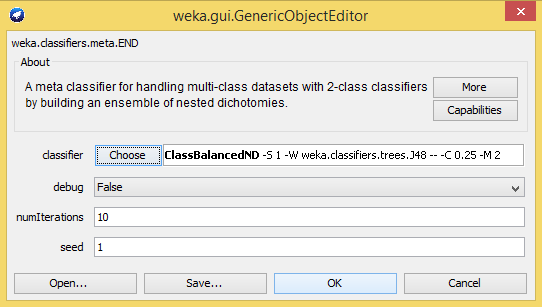
\includegraphics[width=9cm, height=5cm]{images/altera_end}}
	\caption {Alteração de classificador no algoritmo de meta-aprendizagem \textit{END}.}
	\label{end}
\end{figure}

Através das regras utilizadas pelo algoritmo, pode-se constatar que foram classificados corretamente como desligado:

\begin{itemize}
	\item 100\% dos alunos reprovados com menção TR ou TJ, 90,91\% com menção SR, 96,72\% com menção II e 74,36\% que obtiveram crédito concedido em Computação Básica;
	\item 61,75\% dos alunos reprovados com menção MI, 95,17\% com menção SR, 68,36\% com menção II e 95,16\% com menção TR em Física 3, dada a aprovação em Computação Básica com menção SS;
	\item 73,24\% dos alunos aprovados com menção MM em Computação Básica e Física 2 e reprovados com menção SR em Cálculo 3;
	\item  68,31\% dos alunos reprovados com menção MI, 95,15\% com menção II, 95,15\% com menção SR e 95,16\% com menção SR em Física 2, dada a aprovação em Computação Básica com menção MM;
	\item 66,26\% dos alunos reprovados com menção MI, 96,67\% com menção II e 96,54\% com menção SR em Física 2, dada a aprovação em Computação Básica com menção MS;
	\item 57,10\% dos alunos reprovados com menção MI, 100\% com menção SR e 73,82\% com menção II em Estruturas de Dados, dada a aprovação em Computação Básica e Física 2 com menção MS.
\end{itemize}

Analisando as taxas de classificação geradas pelos algoritmos conforme mostrado na Tabela \ref{cursando_geral}, foi possível identificar que entre os alunos que estavam cursando em 2014, 30\% a 54\% foram classificados como desligados, enquanto que 24\% a 31\% foram considerados formados, indicando que os alunos têm maior propensão a serem desligados do curso antes da conclusão. Considerando a taxa de desligamento, 30,06\% dos alunos irão desligar-se no melhor caso e 53,99\% no pior caso. Considerando a taxa de formatura, 30,67\% dos alunos irão formar-se no melhor caso e 24,54\% no pior caso. Para ambos os casos, o algoritmo \textit{DecisionTable} apresentou a maior taxa de predição para prováveis formados e desligados.

\begin{table} [!h]
	\centering
	\caption{Análise das matrizes de confusão dos algoritmos para os alunos identificados como cursando em 2014.} 
	\begin{tabular}{C{5cm}|C{3cm}C{3cm}C{3cm}}
		\hline
		\multicolumn{1}{c}{Algoritmo} & \multicolumn{3}{|c}{Percentual (\%) de classificação dos cursandos em 2014}\\ \hline
		& Formado & Desligado & Cursando\\
		\hline
		J48 &  24,54 & 30,06 & 45,40\\
		J48graft & 24,54 & 30,37 & 45,09 \\
		DecisionTable & 30,67 & 53,99 & 15,34 \\
		PART & 27,91 & 32,31 & 39,78 \\
		AttributteSelectedClassifier & 26,07 & 32,82 & 41,11\\
		END & 27,91 & 49,39 & 22,70\\	
		\hline
	\end{tabular}
	\label{cursando_geral}
\end{table}

A partir dos algoritmos de clusterização \textit{SimpleKMeans} e \textit{FatherstFirst}, foi realizada a análise dos \textit{clusters} gerados a partir dos atributos \textit{AluSexo} e \textit{AluSituacao}. Pelo algoritmo \textit{SimpleKMeans}, foram gerados dois \textit{clusters}, onde  63\% das instâncias pertencem ao \textit{cluster} 0 e o ponto centroide é representado pelos alunos do sexo masculino formados. Em 37\% das instâncias pertencem ao \textit{cluster} 1 e  o ponto centroide é representado pelos alunos do sexo masculino desligados, conforme mostrado na Figura \ref{cluster-kmeans}.

\begin{figure}[!h]
	\centering
	{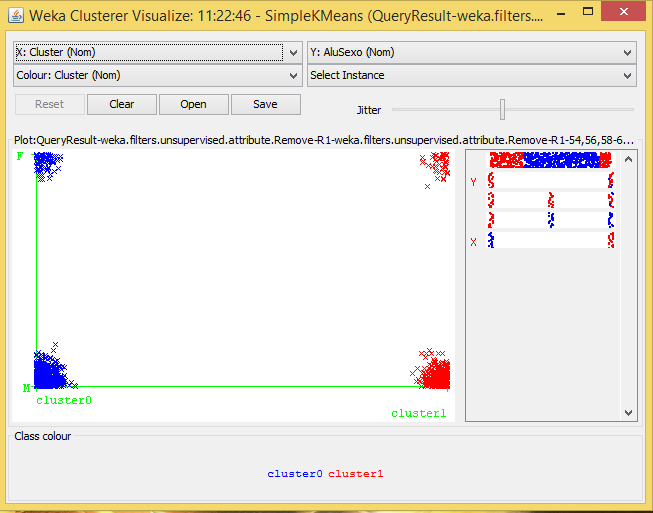
\includegraphics[width=10cm, height=8cm]{images/cluster-kmeans}}
	\caption {\textit{Cluster} gerado pelo algoritmo \textit{SimpleKmeans}, a partir dos atributos \textit{AluSexo} e \textit{AluSituacao}.}
	\label{cluster-kmeans}
\end{figure}
 
 O algoritmo \textit{FatherstFirst} também gerou dois \textit{clusters}, onde 41\% das instâncias pertencem ao \textit{cluster} 0, e o ponto centroide é representado pelos alunos do sexo feminino formado, e  59\% das instâncias pertencem ao \textit{cluster} 1 e o ponto centroide é representado pelos alunos do sexo masculino desligados, conforme mostrado na Figura \ref{cluster-first}.
 
 \begin{figure}[!h]
 	\centering
 	{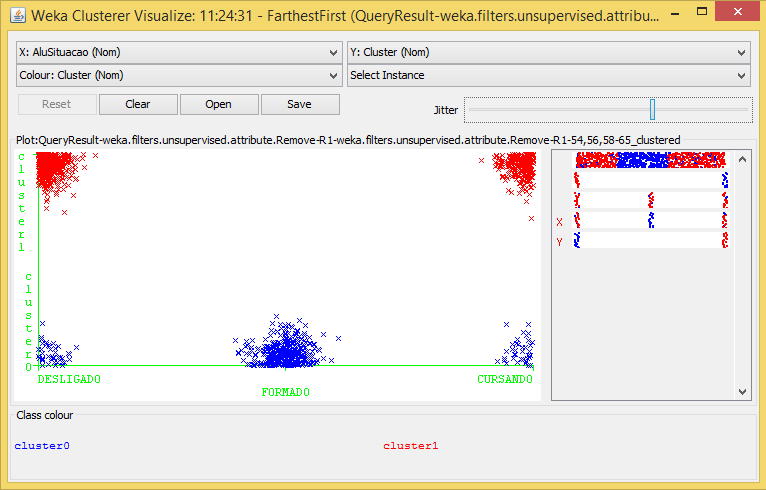
\includegraphics[width=10cm, height=8cm]{images/cluster-first}}
 	\caption {\textit{Cluster} gerado pelo algoritmo \textit{FatherstFisrt}, a partir dos atributos \textit{AluSexo} e \textit{AluSituacao}.}
 	\label{cluster-first}
 \end{figure}
 
\subsection{Evasão dos Alunos nos Semestres com Maiores Taxas de Desligamento} \label{resultado2}

Para a análise dos dados por semestre de ingresso, foram selecionados os algoritmos que apresentaram os melhores conjuntos de regras (que utilizaram maior número de atributos no conjunto de regras ou que apresentaram padrões precisos) e que apresentaram maiores taxas de acerto, considerando o número de instâncias que foram classificadas corretamente e a estatística \textit{Kappa} dos algoritmos, que mede a precisão de predição de uma classe verdadeira. A Estatística \textit{Kappa} varia entre 0 e 1, considerando que quanto mais próximo do valor 1 melhor o desempenho do algoritmo na classificação das instâncias. Pelo fato de cada algoritmo gerar uma regra específica para classificação, buscou-se comparar as regras e identificar similaridades nos padrões de regras utilizadas pelos algoritmos selecionados. 

\subsubsection{Ingressantes no Segundo Semestre de 2002}
Para o conjunto de dados do segundo semestre de 2002, os algoritmos que apresentaram as melhores regras e melhor desempenho foram os algoritmos de árvore \textit{ADTree, BFTree e LADTree}, o algoritmo de regras \textit{JRip} e os algoritmos de meta-aprendizagem \textit{Bagging, MultiBoostAB} e \textit{RandomCommitee}, conforme mostrado na Tabela \ref{algoritmos2_2002}.

\begin{table} [!h]
	\centering
	\caption{Algoritmos utilizados para os dados do segundo semestre de 2002.} 
	\begin{tabular}{C{3,5cm}|C{3,5cm}C{3,5cm}C{3,5cm}}
		\hline
		\multicolumn{1}{c}{Algoritmo} & \multicolumn{3}{|c}{Critérios de Avaliação}\\ \hline
		 & Instâncias Classificadas Corretamente (\%) & Instâncias Classificadas Incorretamente (\%) & Estatística \textit{Kappa}\\
		\hline
		ADTree &  85.7143 & 14.2857 & 0.7126\\
		BFTree & 88.5714 & 11.4286 & 0.7705\\
		LADTree & 94.2857 & 5.7143 & 0.8852\\
		JRip & 88.5714 & 11.4286 & 0.7697\\
		Bagging & 88.5714 & 11.4286 & 0.7697\\
		MultiBoostAB & 91.4286 & 8.5714 & 0.8276\\
		RandomCommitee & 88.5714 & 11.4286 &  0.7697\\
		
		\hline
	\end{tabular}
	\label{algoritmos2_2002}
\end{table}

Para o segundo semestre de 2002, uma das causas percebidas para justificar a evasão dos alunos foi a reprovação na disciplina de Computação Básica, dado que os algoritmos \textit{LADTree}, \textit{JRIP} e \textit{MultiBoostAB} classificaram os alunos que cursaram a disciplina Computação Básica mais de uma vez como desligados. Pelo algoritmo \textit{MultiBoostAB}, alunos que cursaram Computação Básica mais de uma vez foram identificados como desligados numa proporção de 100\%.

Uma exceção encontrada pelos algoritmos \textit{ADTree, BFTree}, \textit{LADTree}, e \textit{Bagging} e \textit{RandomCommitee} foi que os alunos que foram aprovados em Cálculo 2 pela primeira vez, com menção SS, foram identificados com desligados. Pelo algoritmo \textit{BFTree}, foram identificados três casos nesta condição no conjunto de teste gerado pelo algoritmo. Uma das possibilidades para justificar tal regra é o fato do conjunto de dados constituir uma amostra pequena.

Para o algoritmo \textit{ADTree}, as alunas foram classificados como desligadas. Para o algoritmo \textit{RandomCommitee}, os alunos que obtiveram SR como primeira menção em Física 3, MM como última menção em Programação Sistemática ou a última menção em Física 2 diferente de MM apresentaram maior probabilidade de serem classificados como desligados. O mesmo ocorre para a disciplina de Computação Básica, na qual alunos que obtiveram menção MI ao cursar a disciplina pela primeira vez foram classificados como desligados, conforme as regras geradas pelos algoritmos \textit{LADTree, Bagging, MultiBoostAB} e \textit{RandomComitee}, o que indica que o desempenho do  aluno na disciplina de Computação Básica foi um dos determinantes para o desligamento do aluno. 

Conforme a Tabela \ref{algoritmos2_2002}, o algoritmo de árvore de decisão \textit{LADTree} apresentou o melhor desempenho. A Figura \ref{ladtree2_2002} apresenta a regra de classificação utilizada pelo algoritmo, onde aproximadamente 94,3\% das instâncias foram classificadas corretamente.
 
 \begin{figure}[!h]
 	\centering
 	{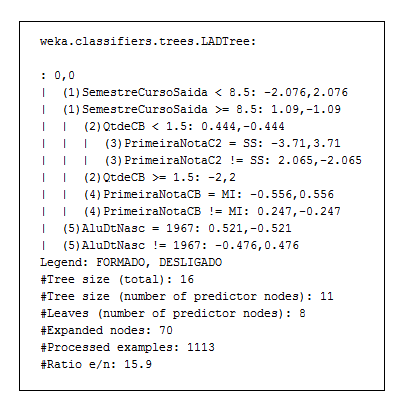
\includegraphics[width=8cm, height=8cm]{images/regra2_2002}}
 	\caption {Regra gerada pelo algoritmo de árvore \textit{LADTree}. Os valores positivos indicam se o aluno está formado ou desligado, conforme condição.}
 	\label{ladtree2_2002}
 \end{figure}
 
 
\subsubsection{Ingressantes no Primeiro Semestre de 2004}

Para o primeiro semestre de 2004, os algoritmos que apresentaram melhores desempenhos foram os algoritmos de árvore \textit{ADTree, J48graft} e \textit{LADTree}, o algoritmo de regras {OneR} e os algoritmos de meta-aprendizagem \textit{Bagging, MultiBoostAB} e \textit{RandomCommitee}, conforme apresentado na Tabela \ref{algoritmos1_2004}.

\begin{table} [!h]
	\centering
	\caption{ Algoritmos Utilizados para os dados do primeiro semestre de 2004.} 
	\begin{tabular}{C{3,5cm}|C{3,5cm}C{3,5cm}C{3,5cm}}
		\hline
		\multicolumn{1}{c}{Algoritmo} & \multicolumn{3}{|c}{Critérios de Avaliação}\\ \hline
		& Instâncias Classificadas Corretamente (\%) & Instâncias Classificadas Incorretamente (\%) & Estatística \textit{Kappa}\\
		\hline
		ADTree & 69.4444 & 30.5556 & 0.3125\\
		J48graft & 72.2222 & 27.7778 & 0.4156\\
		LADTree & 72.2222 & 27.7778 & 0.4156\\
		OneR & 66.6667 & 33.3333 & 0.3165\\
		Bagging &  77.7778 & 22.2222 & 0.5325\\
		MultiBoostAB & 75 & 25 & 0.4671\\
		RandomCommitee & 75 & 25 & 0.4527\\
		\hline
	\end{tabular}
	\label{algoritmos1_2004}
\end{table}

Todos os algoritmos apresentados na Tabela \ref{algoritmos1_2004} utilizaram atributos da disciplina Cálculo 3 em suas regras, em que alunos que foram aprovados em Cálculo 3 foram classificados como formados. Pela regra utilizada pelo algoritmo \textit{OneR}, os alunos que obtiveram menções MM e MS estão formados, e para as demais menções (II, TR, SR e SS) os alunos foram classificados como desligados. Em 88,89\% das instâncias foram classificadas corretamente neste caso.

Pelos algoritmos \textit{LADTree, Bagging } e \textit{MultiBoostAB}, os alunos que obtiveram MI como primeira menção na disciplina Estruturas de Dados foram classificados como desligados. Ainda para a disciplina Estruturas de Dados, o algoritmo \textit{J48graft} determinou que dada a aprovação do aluno em Cálculo 3, se o aluno cursou a disciplina mais de uma vez, este foi considerado desligados.

Para a disciplina Cálculo 2, foi verificado que os alunos que obtiveram MM como última nota foram classificados como desligados pelos algoritmos \textit{ADTree, LADTree} e \textit{MultiBoostAB}. Pelo algoritmo \textit{MultiBoostAB}, alunos que obtiveram MM como última menção em Cálculo 2 foram classificados em 89,95\% como desligados. 

Para a disciplina Programação Sistemática, os algoritmos \textit{ADTree, LADTree} e \textit{MultiBoostAB}, os alunos que obtiveram menção MS foram classificados como formados. Para as demais menções, o algoritmo \textit{MultiBoostAB} determinou em 77,88\% como desligados.

Para o primeiro semestre de 2004, a nota obtida em Cálculo 2 aparenta ser um dos fatores determinantes para a continuidade dos alunos ingressantes no semestre, o que pode indicar uma relação entre o desempenho do aluno em Cálculo 2 para Cálculo 3, visto que todos os algoritmos utilizaram a aprovação em Cálculo 3 como regra de classificação dos alunos. Outra justificativa é o fato de muitos alunos terem cursado Cálculo 3 nos semestres finais do curso, o que implica para os algoritmos que se o aluno não cursou Cálculo 3 ou obteve baixo desempenho, foram considerados desligados. Do mesmo modo, a aprovação na disciplina Estruturas de dados pode ser considerada um fator de decisão, já que os algoritmos também indicaram que alunos que cursaram Estruturas de Dados mais de uma vez foram classificados como desligados.  

Conforme a Tabela \ref{algoritmos1_2004}, o algoritmo que apresentou o melhor desempenho foi o algoritmo de regra \textit{Bagging}, onde aproximadamente 77,8\% das instâncias foram classificadas corretamente. Ao todo, foram geradas 10 árvores de decisão distintas pelo algoritmo. A Figura \ref{regra1_2004} apresenta uma delas como exemplo.

 \begin{figure}[!h]
 	\centering
 	{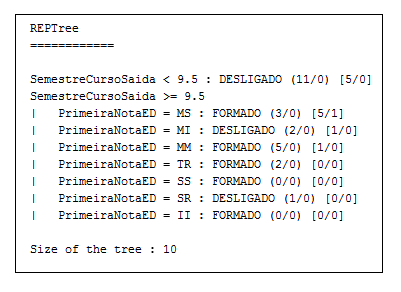
\includegraphics[width=9cm, height=6.5cm]{images/regra1_2004}}
 	\caption {Uma das regras geradas pelo algoritmo de regras \textit{Bagging} para os dados do primeiro semestre de 2004.}
 	\label{regra1_2004}
 \end{figure}

\subsubsection{Ingressantes no Segundo Semestre de 2005}

Para os dados do segundo semestre de 2005, foram utilizados os algoritmos de árvore \textit{ADTree, BFTree, LADTree} e \textit{SimpleCart}, e os algoritmos de meta-aprendizagem \textit{AdaBoostM1, MultiBoostAB} e \textit{RandomSubSpace}, conforme apresentado na Tabela \ref{algoritmos2_2005}. Os algoritmos de regras não foram considerados, por não apresentarem novas regras e padrões desconhecidos para o conjunto de dados.

\begin{table} [!h]
	\centering
	\caption{ Algoritmos Utilizados para os dados do segundo semestre de 2005.} 
	\begin{tabular}{C{3,5cm}|C{3,5cm}C{3,5cm}C{3,5cm}}
		\hline
		\multicolumn{1}{c}{Algoritmo} & \multicolumn{3}{|c}{Critérios de Avaliação}\\ \hline
		& Instâncias Classificadas Corretamente (\%) & Instâncias Classificadas Incorretamente (\%) & Estatística \textit{Kappa}\\
		\hline
		ADTree &  86.8421 & 13.1579 & 0.7383\\
		BFTree & 69.4444 & 30.5556 &  0.4\\
		LADTree & 72.2222 & 27.7778 &  0.4714\\
		SimpleCart & 69.4444 & 30.5556 & 0.489\\
		AdaBoostM1 & 72.2222 & 27.7778 & 0.4578\\
		MultiBoostAB & 75 & 25 & 0.5207\\
		RandomSubSpace & 72.2222 & 27.7778 & 0.4643\\
		\hline
	\end{tabular}
	\label{algoritmos2_2005}
\end{table}

Um padrão identificado, em todos os algoritmos, foi a utilização do atributo referente à ultima turma de Cálculo 2 nas regras de classificação. Em todas as regras geradas, foram classificados como formados os alunos que cursaram Cálculo 2 na turma K no primeiro semestre de 2006. Outro padrão identificado pelos algoritmos \textit{ADTree, LADTree, AdaBoostM1} e \textit{MultiBoostAB} é que alunos que obtiveram SR como primeira menção na disciplina Física 3 foram identificados como desligados. Todos os algoritmos de árvore de decisão classificaram como desligados os alunos que saíram antes do ano de 2007.

Pelo algoritmo \textit{LADTree} e \textit{AdaBoostM1}, foram classificados como formados os alunos que cursaram Física 2 na turma K no primeiro semestre de 2006. Pelos algoritmos \textit{ADTree, LADTree} e \textit{AdaBoostM1}, alunos que obtiveram a primeira menção em Estruturas de Dados diferente de MM foram considerados desligados. 

Para os dados deste semestre, as turmas nas quais foram cursadas as disciplinas de Cálculo 2 e o desempenho na disciplina Estruturas de Dados foram os fatores que mais influenciaram na continuidade dos alunos. Outra tendência percebida é que os alunos que obtêm SR ao cursar Física 3 pela primeira vez têm maior propensão a evadir do curso, o que pode indicar uma dificuldade por parte dos alunos para a disciplina. Ao analisar as turmas de Cálculo 2, percebe-se que vários fatores podem estar relacionados ao desempenho da turma, que podem estar relacionados ao conteúdo, ao docente (didática empregada, formas de avaliação, entre outros), ou ao aluno (motivação, tempo dedicado aos estudos, facilidade ou dificuldade de assimilação dos conteúdos), o que exige uma estudo mais detalhado e aprofundado.

Dos algoritmos utilizados, o que apresentou o melhor desempenho foi o \textit{ADTree}, pois aproximadamente 86,8\% das instâncias foram classificadas corretamente. A regra gerada é apresentada na Figura \ref{regra2_2005}. 

 \begin{figure}[!h]
 	\centering
 	{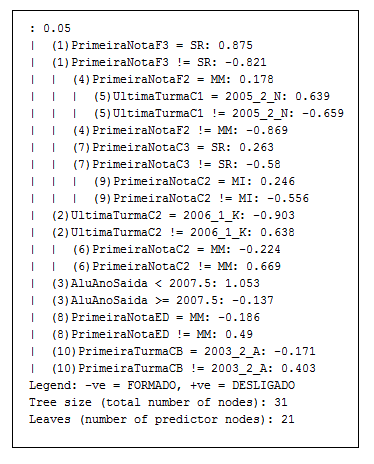
\includegraphics[width=11cm, height=11cm]{images/regra2_2005}}
 	\caption {Regra gerada pelo algoritmo de árvore de decisão \textit{ADTree} para os dados do segundo semestre de 2005.}
 	\label{regra2_2005}
 \end{figure}


\subsubsection{Ingressantes no Primeiro Semestre de 2006}

Para os dados do primeiro semestre de 2006, foram utilizados os algoritmos de árvore \textit{ADTree, BFTree, LADTree} e \textit{SimpleCart}, e os algoritmos de meta-aprendizagem \textit{Bagging, LogitBoost} e \textit{MultiBoostAB}, conforme apresentado na Tabela \ref{algoritmos1_2006}. Os algoritmos de regras não foram utilizados para a análise deste conjunto.

\begin{table} [!h]
	\centering
	\caption{ Algoritmos Utilizados para os dados do primeiro semestre de 2006.} 
	\begin{tabular}{C{3,5cm}|C{3,5cm}C{3,5cm}C{3,5cm}}
		\hline
		\multicolumn{1}{c}{Algoritmo} & \multicolumn{3}{|c}{Critérios de Avaliação}\\ \hline
		& Instâncias Classificadas Corretamente (\%) & Instâncias Classificadas Incorretamente (\%) & Estatística \textit{Kappa}\\
		\hline
		ADTree &  80 & 20 & 0.604\\
		BFTree & 82.5 & 17.5 &  0.6552\\
		LADTree & 85 & 15 & 0.703\\
		SimpleCart & 82.5 & 17.5 & 0.6552\\
		Bagging & 82.5 & 17.5 & 0.6517\\
		LogitBoost & 80 & 20 &  0.6\\
		MultiBoostAB & 82.5 & 17.5 & 0.6552\\
		\hline
	\end{tabular}
	\label{algoritmos1_2006}
\end{table}

Todos os algoritmos, com exceção dos algoritmos \textit{Bagging} e \textit{MultiBoostAB}, utilizaram atributos relacionados à disciplina Física 3 em suas regras de classificação. Pelos algoritmos de árvore de decisão, os alunos que cursaram Física 3 na turma D no segundo semestre de 2007 foram classificados como formados. Junto à disciplina de Física 3, a aprovação em Programação Sistemática foi utilizada pelos algoritmos \textit{ADTree, LogitBoost} e \textit{MultiBoostAB}, no qual alunos que obtiveram menção MS foram classificados como formados, e os alunos que obtiveram menções diferente de MS foram classificados como desligados. Pelo algoritmo \textit{MultiBoostAB}, alunos que obtiveram menção MS na disciplina Programação Sistemática foram classificados em 79,93\% dos casos como formados. Alunos que foram aprovados em Física 3 e Cálculo 3 foram classificados como aprovados.

Pela análise dos algoritmos e das regras geradas, percebe-se que a maior dificuldade dos alunos encontra-se nas disciplinas do terceiro semestre do curso, tais como Física 3 e Programação Sistemática, o que pode indicar que nesse grupo os alunos obtiveram um bom desempenho nos dois primeiros semestres.

O algoritmo \textit{LADTree} apresentou o melhor desempenho para os dados do primeiro semestre de 2006, pois 85\% das instâncias foram classificadas corretamente. A regra gerada pelo algoritmo é mostrada na Figura \ref{regra1_2006}. 


 \begin{figure}[!h]
 	\centering
 	{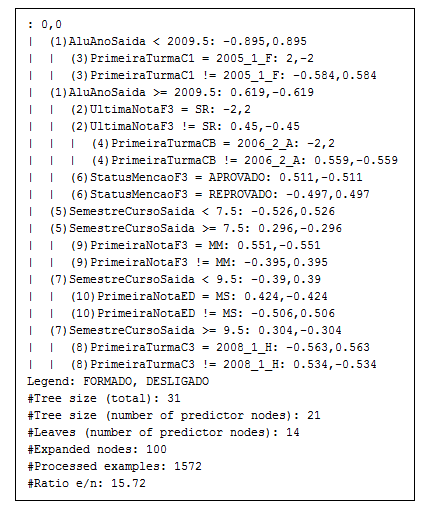
\includegraphics[width=10cm, height=12cm]{images/regra1_2006}}
 	\caption {Regra gerada pelo algoritmo de árvore \textit{LADTree} para os dados do primeiro semestre de 2006.}
 	\label{regra1_2006}
 \end{figure}

\subsubsection{Ingressantes no Segundo Semestre de 2006}

Para os dados do segundo semestre de 2006, foram utilizados os algoritmos de árvore \textit{BFTree, J48, J48graft} e \textit{LADTree}, o algoritmo de regra \textit{Ridor} e os algoritmos de meta-aprendizagem \textit{FilteredClassifier} e \textit{RandomCommittee}, conforme apresentado na Tabela \ref{algoritmos2_2006}.

\begin{table} [!h]
	\centering
	\caption{ Algoritmos Utilizados para os dados do segundo semestre de 2006.} 
	\begin{tabular}{C{3,5cm}|C{3,5cm}C{3,5cm}C{3,5cm}}
		\hline
		\multicolumn{1}{c}{Algoritmo} & \multicolumn{3}{|c}{Critérios de Avaliação}\\ \hline
		& Instâncias Classificadas Corretamente (\%) & Instâncias Classificadas Incorretamente (\%) & Estatística \textit{Kappa}\\
		\hline
		BFTree &  86.1111 & 13.8889 & 0.7309\\
		J48 & 83.3333 & 16.6667 &  0.6776\\
		J48graft & 83.3333 & 16.6667 &  0.6776\\
		LADTree & 86.1111 & 13.8889 & 0.7293\\
		Ridor & 86.1111 & 13.8889 & 0.7309\\
		FilteredClassifier & 86.1111 & 13.8889 &   0.7309\\
		RandomCommittee & 83.3333 & 16.6667 & 0.6766\\
		\hline
	\end{tabular}
	\label{algoritmos2_2006}
\end{table}

Os algoritmos \textit{BFTree, J48, FilterClassifier} e \textit{RandomCommitee} utilizaram a primeira turma da disciplina Estruturas de Dados para classificar os alunos como formados ou desligados, porém os algoritmos \textit{BFTree} e \textit{FilteredClassifier} apresentaram melhores desempenhos, ambos classificando aproximadamente 86,1\% das instâncias corretamente. Comparando as duas regras geradas, os alunos que cursaram Estruturas de Dados pela primeira vez na turma E no primeiro semestre de 2010, na turma A no primeiro semestre de 2008 ou na turma C no segundo semestre de 2004 foram classificados como desligados, dado que o aluno saiu do curso depois do ano de 2009. Pelo algoritmo \textit{J48graft}, o aluno que cursou Estruturas de Dados na turma C no segundo semestre de 2004 foi classificado como desligado dado que o aluno não tenha cursado Física 1 na turma A no segundo semestre de 2006.

Pelos algoritmos \textit{J48graft} e \textit{LADTree}, os alunos que cursaram Física 1 na turma A no segundo semestre de 2006 foram classificados como formados, da mesma forma que os alunos que cursaram Cálculo 2 na turma K no primeiro semestre de 2007 e os alunos que cursaram Física 1 na turma A no segundo semestre de 2006. Pelos algoritmos \textit{LADTree} e \textit{RandomCommittee}, alunos que foram aprovados em Cálculo 1 ao cursar a disciplina pela primeira vez foram classificados como aprovados.

Analisando as regras apresentadas, percebe-se que os atributos relacionados à disciplina Estruturas de Dados foram utilizados pela maioria dos algoritmos, o que indica que a turma na qual o aluno cursou a disciplina pela primeira vez pode estar influenciando no desempenho posterior do aluno, seja de forma direta ou indireta.

Entre os algoritmos utilizados, o \textit{BFTree, Ridor} e \textit{FilteredClassifier} apresentaram melhores desempenhos, ambos identificado aproximadamente 86,1\% das instâncias classificadas corretamente. A Figura \ref{regra2_2006} apresenta a regra de classificação gerada pelo algoritmo \textit{FilteredClassifier}. Os números entre parênteses representam, respectivamente, o número de instâncias abrangidas pela regra e o número de instâncias classificadas incorretamente, ambos separados por uma barra.

 \begin{figure}[!h]
 	\centering
 	{\includegraphics[width=11cm, height=10cm]{images/regra2_2006}}
 	\caption {Regra gerada pelo algoritmo de meta-aprendizagem \textit{FilteredClassifier} para os dados do segundo semestre de 2006.}
 	\label{regra2_2006}
 \end{figure}


\subsubsection{Ingressantes no Segundo Semestre de 2009}

Para os dados do segundo semestre de 2009, foram utilizados o algoritmo de árvore \textit{J48graft}, o algoritmo de regras \textit{JRip} e os algoritmos de meta-aprendizagem \textit{AdaBoostM1, Bagging, Decorate} e \textit{LogitBoost}, conforme apresentado na Tabela \ref{algoritmos2_2009}.

\begin{table} [!h]
	\centering
	\caption{ Algoritmos Utilizados para os dados do segundo semestre de 2006.} 
	\begin{tabular}{C{3,5cm}|C{3,5cm}C{3,5cm}C{3,5cm}}
		\hline
		\multicolumn{1}{c}{Algoritmo} & \multicolumn{3}{|c}{Critérios de Avaliação}\\ \hline
		& Instâncias Classificadas Corretamente (\%) & Instâncias Classificadas Incorretamente (\%) & Estatística \textit{Kappa}\\
		\hline
		J48graft &  93.75 & 6.25 & 0.8822\\
		JRip &  97.9167 & 2.0833 &  0.962\\
		AdaBoostM1 & 89.5833 & 10.4167 & 0.8098\\
		Bagging & 93.75 & 6.25 & 0.8822\\
		Decorate & 93.75 & 6.25 & 0.8822\\
		LogitBoost & 91.6667 & 8.3333 & 0.8502\\
		\hline
	\end{tabular}
	\label{algoritmos2_2009}
\end{table}

Os algoritmos \textit{J48graft, Bagging} e \textit{LogitBoost} identificaram os alunos que foram aprovados com menção MM em Física 1 como desligados. Pelo algoritmo \textit{AdaBoost}, alunos aprovados com menção MM em Física 1 foram classificados em 57,61\% como desligados. Outro padrão identificado pelos algoritmos é que alunos que cursaram a disciplina Programação Sistemática na turma A no segundo semestre de 2010 foram classificados como formados.

Por meio das regras apresentadas, o desempenho na disciplina de Física 1 pode ser considerada um fator determinante no processo de evasão, visto que por ser uma disciplina inicial, a não aprovação nesta disciplina ou um baixo rendimento, mesmo o aluno sendo aprovado, poderá impactar nas disciplinas subsequentes.

O algoritmo que apresentou o melhor desempenho para os dados do segundo semestre de 2009 foi o \textit{JRip}, onde aproximadamente 97,9\% das instâncias foram classificadas corretamente. A Figura \ref{regra2_2009} apresenta a regra de classificação utilizada pelo algoritmo.

 \begin{figure}[!h]
 	\centering
 	{\includegraphics[width=11cm, height=4cm]{images/regra2_2009}}
 	\caption {Regra gerada pelo algoritmo de regras \textit{JRip} para os dados do segundo semestre de 2009.}
 	\label{regra2_2009}
 \end{figure}

\subsubsection{Ingressantes no Segundo Semestre de 2011}

Para os dados do segundo semestre de 2011, foram utilizados o algoritmo de árvore \textit{LADTree}, o algoritmo de regra \textit{JRip} e os algoritmos de meta-aprendizagem \textit{Bagging, FilteredClassifier, MultiBoostAB, OrdinalClassClassifier} e \textit{RandomSubSpace}, conforme apresentado na Tabela \ref{algoritmos2_2011}.


\begin{table} [!h]
	\centering
	\caption{ Algoritmos Utilizados para os dados do segundo semestre de 2011.} 
	\begin{tabular}{C{3,5cm}|C{3,5cm}C{3,5cm}C{3,5cm}}
		\hline
		\multicolumn{1}{c}{Algoritmo} & \multicolumn{3}{|c}{Critérios de Avaliação}\\ \hline
		& Instâncias Classificadas Corretamente (\%) & Instâncias Classificadas Incorretamente (\%) & Estatística \textit{Kappa}\\
		\hline
		LADTree & 80.4348 & 19.5652 & 0.6057\\
		JRip & 86.9565 & 13.0435 & 0.7386\\
		Bagging & 82.6087 & 17.3913 & 0.6515\\
		FilteredClassifier & 86.9565 & 13.0435 & 0.7386\\
		MultiBoostAB & 82.6087 & 17.3913 & 0.6515\\
		OrdinalClassClassifier & 86.9565 & 13.0435 & 0.7386\\
		RandomSubSpace & 82.6087 & 17.3913 & 0.6515\\
		\hline
	\end{tabular}
	\label{algoritmos2_2011}
\end{table}

Todos os algoritmos utilizaram a disciplina Física 1 como ponto de análise inicial. Através dos algoritmos \textit{Bagging} e \textit{RandomSubSpace}, os alunos com menções MI, II e SR em Física 1 foram classificados como desligados. Dado que o aluno foi aprovado em Física 1, a aprovação em Programação Sistemática foi determinante para classificar se o aluno está cursando ou desligado. Pelos algoritmos \textit{LADTree} e \textit{MultiBoostAB}, alunos que obtiveram SR em Programação Sistemática foram classificados como desligados.

Analisando os padrões detectados pelos algoritmos, as disciplinas de Física 1 e Programação Sistemática foram determinantes para os algoritmos classificarem o aluno como cursando ou desligado. Dado que todos os algoritmos identificaram Física 1 como origem das regras, percebe-se que os alunos ingressantes nesse semestre encontraram dificuldades na disciplina.

Os algoritmos que apresentaram os melhores desempenhos foram  \textit{JRip, FilteredClassifier} e o \textit{OrdinalClassClassifier}, pois ambos classificaram aproximadamente 87\% das instâncias corretamente. Analisando as matrizes de confusão dos algoritmos, 3 alunos cursando foram identificados como desligados e 3 alunos desligados foram identificados como cursando. A Figura \ref{regra2_2011} apresenta a regra de classificação utilizada pelo algoritmo \textit{JRip}. 

 \begin{figure}[!h]
 	\centering
 	{\includegraphics[width=11cm, height=4cm]{images/regra2_2011}}
 	\caption {Regra gerada pelo algoritmo de regras \textit{JRip} para os dados do segundo semestre de 2011.}
 	\label{regra2_2011}
 \end{figure}
  

\chapter{Conclusão} \label{chapter7}

Neste trabalho, foram identificadas variáveis, regras e padrões capazes de auxiliar na detecção das causas de evasão dos alunos do Bacharelado em Ciência da Computação. Foram realizadas análises estatísticas e mineração de dados a partir dos dados disponibilizados sobre os alunos ingressantes no curso entre 2000 e 2013.

Foi verificado que, embora a taxa de ingresso tenha crescido ao longo dos anos, a quantidade de alunos que evadiram do curso é bastante superior à quantidade de alunos formados. O percentual de alunas formadas é superior ao de alunos formados, embora o ingresso de alunos seja muito predominante. A partir de 2008, é verificado um decréscimo na taxa de formados por semestre de ingresso, visto que a maioria dos alunos levam mais de 10 semestres para concluir o curso. Para os alunos (do sexo masculino), não foi identificado um período com maior índice de evasão, enquanto que para as alunas a evasão é maior entre o primeiro e o terceiro semestres do curso.

Foi verificado que o vestibular e o PAS constituem as principais formas de ingresso no curso. Os percentuais de ingresso e desligamento do vestibular são maiores se comparados aos do PAS. Não constatou-se, entre 2000 e 2013, alunos formados que ingressaram por matrícula cortesia, convênio internacional e transferência facultativa. Como a Universidade de Brasília adotou o ENEM como forma de ingresso a partir de 2012, ainda não foram constatados alunos formados. 

Entre as formas de desligamento, as principais apontadas foram desligamento por não cumprimento de condição, desligamento por abandono e desligamento voluntário. Foi verificado que os alunos  desligados em geral cursaram, em média, de cinco a seis semestres. Ainda, foi possível verificar para as alunas, uma maior taxa de desligamento entre o primeiro e o terceiro semestres, o que indica que as alunas tendem a ter evasão do curso principalmente nos dois primeiros anos de graduação.

Comparando a média de desempenho dos alunos em geral e dos alunos desligados, verificou-se que os últimos apresentaram maiores taxas de reprovação, se comparados à media geral. Constatou-se que os alunos apresentam maior dificuldade nas disciplinas ofertadas pelo Departamento de Matemática e o Instituto de Física, especialmente em Cálculo 1, Física 1, Cálculo 3 e Física 3, considerando que essas disciplinas apresentaram altas taxas de reprovação. Das disciplinas analisadas ofertadas pelo Departamento de Ciência da Computação, Computação Básica e Programação Sistemática são as disciplinas com maiores taxas de reprovação, porém os percentuais de reprovação são relativamente menores se comparados às disciplinas de Cálculo e Física.
 
Ao realizar a mineração de dados no Weka, os algoritmos de classificação apresentaram variação no desempenho para cada arquivo de dados analisado, sendo necessária a utilização de diferentes algoritmos para identificar padrões e similaridades entre as regras geradas. Durante a mineração de dados, houve algoritmos que, embora apresentassem uma alta taxa de acerto, não forneciam regras ou informações relevantes para justificar as causas de evasão.

Analisando os dados gerais, os algoritmos apontaram na maioria dos casos que a reprovação ou um baixo desempenho nas disciplinas de Cálculo 1, Física 1, Cálculo 3 e Física 3 estavam relacionados ao desligamento. Porém foram identificadas algumas exceções, como a condição do aluno ser aprovado em Cálculo 2 com menção SS e Física 2 com menção MS ser considerado desligado pelo algoritmo de regra \textit{PART}. Para a regra, foram verificadas seis instâncias na base de dados geral e três instâncias abrangidas pela regra no conjunto de teste no Weka. Ao verificar a base de dados, os alunos desligados que obtiveram menção SS em Cálculo 2 e MS em Física 2 evadiram principalmente por não cumprimento de condição e desligamento voluntário.

 Outra exceção gerada pelo algoritmo \textit{DecisionTable} é dada a aprovação em Cálculo 3 com menção SS e Física 3 com menção MM o aluno ser classificado como desligado, porém ao verificar a base de dados não foi constatada nenhuma instância abrangida pela regra. Também foi verificado que todos os algoritmos aplicados sobre o conjunto de dados gerais apontaram uma tendência dos alunos a saírem do curso antes da conclusão, visto que todos os algoritmos aplicados sobre o conjunto de dados gerais classificaram mais alunos que estavam cursando em 2014 como prováveis desligados do que formados.

Analisando os dados por semestre de ingresso, foi verificado que os atributos relacionados às turmas e menções foram fortemente utilizados para a geração de regras de classificação pelos algoritmos. Pelos algoritmos de classificação, verificou-se que as turmas nas quais as disciplinas foram cursadas também foram determinantes para classificar determinado aluno como cursando, formado ou desligado, principalmente em Cálculo 2, o que sugere a necessidade de um estudo aprofundado a respeito da relação entre as turmas e a continuidade do curso.  Das regras geradas, observou-se que as causas de evasão são variadas para cada semestre analisado, porém o baixo rendimento nas disciplinas de Cálculo 1, Cálculo 3, Física 1, Física 3, Estruturas de Dados e Programação Sistemática apresentaram-se como as causas de evasão mais recorrentes. 

\section{Contribuições} 

Os processos de mineração de dados e de análise estatística realizados neste trabalho permitiram validar a hipótese apresentada na Seção \ref{1title3}, que era identificar informações relevantes para relacionar padrões descobertos nos dados com o processo de desligamento dos alunos no Bacharelado em Ciência da Computação da Universidade de Brasília.

Em resumo, dos resultados obtidos nesse trabalho, sugerimos que o baixo rendimento nas disciplinas de Cálculo 1, Cálculo 3, Física 1, Física 3 e Programação Sistemática podem ser utilizadas como parâmetros para identificar um aluno com risco de evasão.

\section{Trabalhos Futuros}

Como sugestões para trabalhos futuros, são propostos:

\begin{itemize}

	\item Comparar o desempenho dos alunos matriculados no Bacharelado, Licenciatura e Engenharia da Computação nas disciplinas iniciais ofertadas aos três cursos, tais como Cálculo 1 e 2, Computação Básica e Estruturas de Dados;
	\item Comparar o desempenho dos alunos matriculados no Bacharelado em Ciência da Computação nas disciplinas finais de curso, tais como Organização e Arquitetura de Computadores, \textit{Software} Básico e Sistemas Operacionais;
	\item Analisar novos atributos (por exemplo, dados informados na inscrição do vestibular ou PAS) para identificar novos padrões nos perfis de alunos com risco de evasão;
	\item Repetir o experimento futuramente para avaliar se houve diminuição das taxas de evasão com a implantação do novo Projeto Político Pedagógico no Bacharelado em Ciência da Computação.
\end{itemize}

  

  \postextual
  \bibliographystyle{apalike}
  \bibliography{bibliografia}
	\anexos
	
\chapter{Programa e Pré-Requisitos nas Disciplinas Analisadas} \label{anexo1}

As ementas e pré-requisitos das disciplinas analisadas estão disponibilizadas na Tabela \ref{anexo1-tabela}, conforme disponibilizado no Portal MatriculaWeb da Universidade de Brasília.

\begin{longtable}{C{1,3cm}C{2,5cm}C{6,2cm}C{3,5cm}}
	\caption{Programas e pré-requisitos das disciplinas analisadas.}
	\label{anexo1-tabela} \\
	\hline
	Código &Disciplina & Ementa & Pré-requisito(s)\\
	\hline
	116304 & Computação Básica & \begin{itemize}
		\item Histórico do computador; 
		\item Computadores e a Resolução de Problemas; 
		\item Estruturas de Decisão; 
		\item Vetores e Matrizes; 
		\item Cadeias de Caracteres;
		\item Sub-Algoritmos: Funções e Procedimentos; 
		\item O Estilo de Programação; 
		\item Particularidades da Linguagem Pascal.
	\end{itemize} & Disciplina sem pré-requisitos\\ \hline
	116319 & Estruturas de Dados & \begin{itemize}
		\item Representação e Manipulação de Cadeias;
		\item Estruturas de Dados Lineares;
		\item Listas Lineares Encadeadas;
		\item Estruturas de Dados Não Lineares;
		\item Classificação e Pesquisa em Memória.
	\end{itemize} & 116301 - Computação Básica \newline OU \newline 117234 - Programação Avançada\\ \hline
	113956 & Programação Sistemática & \begin{itemize}
		\item Especificação e Definição de Programas;
		\item Métodos de Programação;
		\item Testes Sistemáticos;
		\item Manutenção de Programas;
		\item Estudo de Caso. 
	\end{itemize}  & 116301 - Computação Básica  \newline OU \newline
	113913 - Introdução a Ciência da Computação\\ \hline
	113034 & Cálculo 1 & \begin{itemize}
		\item Funções de uma Variável Real;
		\item Limite e Continuidade;
		\item Derivada;
		\item Integral;
		\item Aplicações da Integral.
	\end{itemize} & Disciplina sem pré-requisitos\\ \hline
	113042 & Cálculo 2 & \begin{itemize}
		\item Sequências, Séries Numéricas;
		\item Séries de Potências;
		\item Fórmula de Taylor, Estimativa de Resto e Aproximações (Funções de uma Variável);
		\item Equações Diferenciais Ordinárias de Primeira Ordem;
		\item Equações Diferenciais Ordinárias Lineares;
		\item O Método das Séries de Potências;
		\item Transformada de Laplace;
		\item Sistemas Lineares de Equações Diferenciais Ordinárias de Primeiras Ordem.
	\end{itemize} & 113034 - Cálculo 1\\ \hline
	113051 & Cálculo 3 & \begin{itemize}
		\item Vetores no Plano e no Espaço;
		\item Funções de Várias Variáveis;
		\item Fórmula de Taylor, Pontos de Extremos Locais e Absolutos;
		\item Transformações Diferenciáveis;
		\item Integrais Múltiplas;
		\item Integrais de Linha;
		\item Integrais de Superfície, Teorema de Divergência e Teorema de Stokes. 
	\end{itemize} & 113042 - Cálculo 2\\ \hline
	118001 & Física 1 & \begin{itemize}
		\item Medição;
		\item Vetores;
		\item Cinemática da Partícula;
		\item Dinâmica da Partícula;
		\item Trabalho e Energia;
		\item Conservação do Momento Linear;
		\item Colisões;
		\item Cinemática da Rotação;
		\item Equilíbrio de Corpos Rígidos.
	\end{itemize} & Disciplina sem pré-requisitos\\ \hline
	118028 & Física 2 & \begin{itemize}
		\item Dinâmica da Rotação;
		\item Conservação do Momentum Angular;
		\item Oscilações;
		\item Gravitação;
		\item Estática dos Fluídos;
		\item Dinâmica dos Fluídos;
		\item Ondas em Meios Elásticos;
		\item Ondas Sonoras;
		\item Temperatura;
		\item Calor e a Primeira Lei da Termodinâmica;
		\item Teoria Cinética dos Gases;
		\item Entropia e a Segunda Lei da Termodinâmica.
	\end{itemize} & 118001 - Física 1 \newline E \newline 113034 - Cálculo 1\\ \hline
	118044 & Física 3 & \begin{itemize}
		\item Lei de Coulomb;
		\item O Campo Elétrico - Lei de Gauss;
		\item Potencial, Capacitância, Propriedade dos Dielétricos;
		\item Corrente, Resistência e Fem;
		\item Circuitos e Instrumentos de Corrente Contínua;
		\item Forças Magnéticas sobre Condutores de Correntes;
		\item Campo Magnético Produzido por Correntes;
		\item Força Eletromotriz Induzida;
		\item Correntes Alternadas;
		\item Equação de Maxwell.
	\end{itemize} & 118028 - Física 2  E 113042 - Cálculo 2 \newline OU \newline 118206 - Física Geral 2  E 113042 - Cálculo 2\\ \hline
\end{longtable}


	\appendix
	
\chapter{Código Java para cálculo da quantidade de semestres cursados pelos alunos} \label{apendiceA}


\noindent package Dados; \newline
import java.sql.Connection; \newline
import java.sql.DriverManager; \newline
import java.sql.SQLException; 
\newline
\newline
public class Corrige\_Semestre \{ 
\begin{quote}
	private static java.sql.Statement stm; \newline
	private static java.sql.Statement stm2; \newline
	private static java.sql.PreparedStatement pst; \newline
	private static Connection conexao; \newline
	\newline		
	// Função: Estabelece conexao com o banco de dados \newline
	public static Connection ObtemConexao() throws SQLException, ClassNotFoundException \{
	\begin{quote}
		Connection conn = null; \newline
		Class.forName ("com.mysql.jdbc.Driver"); \newline
		conn = DriverManager.getConnection(''jdbc:mysql://localhost:3306/alunos\_cic'', ''root'', '' '' ); \newline
		return conn;
	\end{quote}
	\} \newline
	\newline
	//	Função: Determina quantos semestres o aluno cursou até a saída do curso \newline
	public static void AtualizaSemestreCurso() throws ClassNotFoundException, SQLException \{
	\begin{quote}
		String sql1 = null; \newline
		int valor = 0; \newline
		String sql = "select MatricAluno, anoIngresso, SemestreIngresso, AnoSaida, SemestreSaida from alunos"; \newline
		conexao = ObtemConexao(); \newline
		stm = conexao.createStatement(); \newline
		java.sql.ResultSet Rs = stm.executeQuery(sql); \newline
		while (Rs.next()) \{
			\begin{quote}
				int matricula = Rs.getInt(1); \newline
				int anoIngresso = Rs.getInt(2); \newline
				int semestreIngresso =  Rs.getInt(3); \newline
				int anoSaida = Rs.getInt(4); \newline
				int semestreSaida = Rs.getInt(5); \newline
				if (anoSaida == 9999)\{
				\begin{quote}
					sql1 = "update alunos set semestreSaidaCurso = 100 where matricAluno = " + matricula;
				\end{quote}
				\} else \{
				\begin{quote}
					if (semestreSaida == 9) \{
					\begin{quote}
						sql1 = "update alunos set semestreSaidaCurso = 99 where matricAluno = " + matricula;
					\end{quote}
					\} else \{
					\begin{quote}
						if (semestreIngresso == 1) \{
						\begin{quote}
							valor = ((anoSaida - anoIngresso)*2);
						\end{quote}
						\} 
					\end{quote}
					\begin{quote}
						if (semestreIngresso == 2) \{
						\begin{quote}
							valor = ((anoSaida - anoIngresso)*2) - 1;
						\end{quote}
						\}
					\end{quote}
					\begin{quote}
						if ((semestreSaida == 1 )||(semestreSaida == 0))\{
						\begin{quote}
						valor = valor +1;
						\end{quote}
						\} 
					\end{quote}
					\begin{quote}
						if (semestreSaida == 2) \{
						\begin{quote}
							valor = valor +2;
						\end{quote}
						\} \newline
						sql1 = "update alunos set semestreSaidaCurso =" + valor + "where matricAluno = " + matricula;
					\end{quote}
					\}
				\end{quote}
				\} \newline
				System.out.println(sql1); \newline
				pst = conexao.prepareStatement(sql1); \newline
				pst.execute(); 
			\end{quote}
			\}
			
	\end{quote}
	\}	\newline
	\newline 
	// Método Principal \newline
	public static void main (String[] args) throws ClassNotFoundException, SQLException \{
	\begin{quote}
		AtualizaSemestreCurso();
	\end{quote}	
	\}		
\end{quote}
		\}
	

	
\chapter{Código Java para geração das tabelas \textit{evasao\_cic, evasao\_mat} e \textit{evasao\_fis}} \label{apendiceB}


A mesma estrutura de código foi utilizada para a geração das tabelas \textit{evasao\_cic, evasao\_mat} e \textit{evasao\_fis}, onde apenas o nome da tabela e os códigos das disciplinas foram alterados, seguindo a ordem apresentada na Tabela \ref{tabela-apendice}. 

\begin{table}[!h]
	\centering
	\label{tabela-apendice}
	\caption{Tabelas SQL e Códigos das Disciplinas por Departamento.}
	\begin{tabular}{C{3cm}|C{2cm}C{6cm}}
		\hline
		Tabela SQL & Código & Disciplina\\ \hline
		\multirow{3}{*}{\textit{evasao\_cic}} & 116301 & Computação Básica\\
		& 116319 & Estruturas de Dados\\
		& 113956 & Programação Sistemática\\ \hline
		\multirow{3}{*}{\textit{evasao\_mat}} & 113034 & Cálculo 1\\
		& 113042 & Cálculo 2\\
		& 113051 & Cálculo 3\\ \hline
		\multirow{3}{*}{\textit{evasao\_fis}} & 118001 & Física 1\\
		& 118028 & Física 2\\
		& 118044 & Física 3\\ \hline
	\end{tabular}
\end{table}

A seguir, é apresentado o exemplo utilizado para a geração da tabela \textit{evasao\_cic}. \newline
\newline
\newline
package Dados; \newline
import java.sql.Connection; \newline
import java.sql.DriverManager; \newline
import java.sql.SQLException; \newline
\newline

public class Constroi\_Dados\_CIC \{ 
\begin{quote}
	private static java.sql.Statement stm; \newline
	private static java.sql.Statement stm2; \newline
	private static java.sql.PreparedStatement ps; \newline
	private static Connection conexao; \newline
	\newline
	//	Função: Estabelece conexão com o banco de dados. \newline
	public static Connection ObtemConexao() throws SQLException, ClassNotFoundException\{
		\begin{quote}
		Connection conn = null; \newline
		Class.forName("com.mysql.jdbc.Driver"); \newline
		conn = DriverManager.getConnection(''jdbc:mysql://localhost:3306/alunos\_cic'', ''root'', '' ''); \newline
		return conn;
		\end{quote}
	\}  
	
	\textit{// Função: Insere matricula e quantidade de vezes que um aluno cursou a disciplina de Computação Básica.} \newline
	public static void AtualizaCB() throws ClassNotFoundException, SQLException \{	
	\begin{quote}
		String sql = "select distinct MatricAluno, count(CodDisc) from historico where codDisc = 116301 " \newline
		+ "group by MatricAluno order by MatricAluno asc"; \newline
		conexao = ObtemConexao(); \newline
		stm = conexao.createStatement(); \newline
		java.sql.ResultSet Rs = stm.executeQuery(sql); \newline
		while (Rs.next())\{
		\begin{quote}
			int matricula = Rs.getInt(1); \newline
			int quantidade =  Rs.getInt(2); \newline
			String sqlAtualiza = "insert into evasao\_cic (matricula, QtdeCB) values ("+matricula+","+quantidade+") "; \newline
			ps = conexao.prepareStatement(sqlAtualiza); \newline
			ps.execute(); 
			\end{quote}
		\} \newline
		Rs.close(); \newline
		AtualizaED(); \textit{//Atualiza a quantidade de vezes que a disciplina Estruturas de Dados foi cursada.}\newline
		AtualizaPS(); \textit{//Atualiza a quantidade de vezes que a disciplina Programação Sistemática foi cursada.}\newline
		AtualizaMencoesCIC(); \textit{//Atualiza as menções e turmas de Computação Básica, Estruturas de Dados e Programação Sistemática.}
		\end{quote}
	\} \newline
	
	\textit{// Função: Atualiza a quantidade de vezes que a disciplina Estruturas de Dados foi cursada por um aluno.} \newline
	public static void AtualizaED() throws SQLException, ClassNotFoundException \{
	\begin{quote}
		String sql = "select distinct MatricAluno, count(CodDisc) from historico where codDisc = 116319" \newline
		+ "group by MatricAluno"; \newline
		java.sql.ResultSet Rs = stm.executeQuery(sql); \newline
		while (Rs.next()) \{
		\begin{quote}
			int matricula = Rs.getInt(1); \newline
			int quantidade =  Rs.getInt(2); \newline
			String sqlAtualiza = "update evasao\_cic set QtdeED =" + quantidade + " where matricula =" + matricula; \newline
			ps = conexao.prepareStatement(sqlAtualiza); \newline
			ps.execute();
		\end{quote}
		\} \newline
		Rs.close();
	\end{quote}
	\}\newline
	\newline
	\textit{// Função: Atualiza a quantidade de vezes que a disciplina Programação Sistemática foi cursada por um aluno.} \newline
	public static void AtualizaPS() throws SQLException, ClassNotFoundException \{
	\begin{quote}
		String sql = "select distinct MatricAluno, count(CodDisc) from historico where codDisc = 113956" \newline
		+ "group by MatricAluno"; \newline
		java.sql.ResultSet Rs = stm.executeQuery(sql); \newline
		while (Rs.next()) \{
		\begin{quote}
			int matricula = Rs.getInt(1); \newline
			int quantidade =  Rs.getInt(2); \newline
			String sqlAtualiza = "update evasao\_cic set QtdePS =" + quantidade + " where matricula =" + matricula; \newline
			ps = conexao.prepareStatement(sqlAtualiza); \newline
			ps.execute();
		\end{quote}
		\} \newline
		Rs.close();
	\end{quote}
	\}\newline
	\newline
	\textit{//	Atualiza as primeiras e últimas notas e turmas das disciplinas Computação Básica, Estruturas de Dados e Programação Sistemática para cada aluno}. \newline
	public static void AtualizaMencoesCIC() throws SQLException, ClassNotFoundException\{
	\begin{quote}
		conexao = ObtemConexao(); \newline
		stm2 = conexao.createStatement(); \newline
		String mencaoCB1; \newline
		String turmaCB1; \newline
		String mencaoED1; \newline
		String turmaED1; \newline
		String mencaoCB2; \newline
		String turmaCB2; \newline
		String mencaoED2; \newline
		String turmaED2; \newline
		String mencaoPS1; \newline
		String turmaPS1; \newline
		String mencaoPS2; \newline
		String turmaPS2; \newline
		String sql = "select Matricula from evasao\_cic"; \newline
		java.sql.ResultSet Rs5 = stm2.executeQuery(sql); \newline
		while (Rs5.next() == true)\{
		\begin{quote}
			int matricula = Rs5.getInt(1); \newline
			String sqlAtualizaCB1 = "select mencao, concat(ano,'\_',semestre,'\_',turma) from historico where codDisc=116301 and matricAluno =" + matricula + 
			" order by ano asc, semestre asc limit 1"; \newline
			java.sql.ResultSet Rs1 = stm.executeQuery(sqlAtualizaCB1); \newline
			if (Rs1.next())\{
			\begin{quote}
				mencaoCB1 = Rs1.getString(1); \newline
				turmaCB1 = Rs1.getString(2); 
			\end{quote}
			\} \newline
			else\{
			\begin{quote}
				mencaoCB1 = null; \newline
				turmaCB1 = null; \newline
				\} 
			\end{quote}
			String sqlAtualizaCB2 = "select mencao, concat(ano,'\_',semestre,'\_',turma) from historico where codDisc = 116301 and matricAluno ="
			 + matricula + " order by ano desc, semestre desc limit 1"; \newline
			
			java.sql.ResultSet Rs3 = stm.executeQuery(sqlAtualizaCB2); \newline
				if (Rs3.next())\{
				\begin{quote}
					mencaoCB2 = Rs3.getString(1); \newline
					turmaCB2 = Rs3.getString(2); 
				\end{quote}
				\} else \{
				\begin{quote}
				mencaoCB2 = null; \newline
				turmaCB2 = null; \newline
					\} 
				\end{quote}
			String sqlAtualizaED1 = "select mencao, concat(ano,'\_',semestre,'\_',turma) from historico where codDisc=116319 and matricAluno =" + matricula +
			" order by ano asc, semestre asc limit 1"; \newline
			java.sql.ResultSet Rs2= stm.executeQuery(sqlAtualizaED1); \newline
			if (Rs2.next())\{
			\begin{quote}
				mencaoED1 = Rs2.getString(1); \newline
				turmaED1 = Rs2.getString(2); 
			\end{quote}
			\}
			else\{ 
			\begin{quote}
				mencaoED1 = null; \newline
				turmaED1 = null; \newline
				\} 
			\end{quote}
			String sqlAtualizaED2 = "select mencao, concat(ano,'\_',semestre,'\_',turma) from historico where codDisc = 116319 and matricAluno ="
			 + matricula + " order by ano desc, semestre desc limit 1"; \newline
			java.sql.ResultSet Rs4 = stm.executeQuery(sqlAtualizaED2); \newline
			if (Rs4.next())\{ 
			\begin{quote}
				mencaoED2 = Rs4.getString(1); \newline
				turmaED2 = Rs4.getString(2); 
			\end{quote}
			\} else \{
			\begin{quote}
			mencaoED2 = null; \newline
			turmaED2 =null; \newline
			\} 
			\end{quote}
		String sqlAtualizaPS1 = "select mencao, concat(ano,'\_',semestre,'\_',turma) from historico where codDisc = 116319 and matricAluno =" + matricula + 
		" order by ano asc, semestre asc limit 1"; \newline
		java.sql.ResultSet Rs7= stm.executeQuery(sqlAtualizaPS1); \newline
		if (Rs7.next())\{
		\begin{quote}
			mencaoPS1 = Rs7.getString(1);\newline
			turmaPS1 = Rs7.getString(2);
		\end{quote}
		\} else\{
		\begin{quote}
			mencaoPS1 = null; \newline
			turmaPS1 = null; \newline
			\}
			\end{quote}
		
		String sqlAtualizaPS2 = "select mencao, concat(ano,'\_',semestre,'\_',turma) from historico where codDisc = 116319 and matricAluno ="
		 + matricula + " order by ano desc, semestre desc limit 1"; \newline
		java.sql.ResultSet Rs6 = stm.executeQuery(sqlAtualizaED2); \newline
		if (Rs6.next())\{
		\begin{quote}
			mencaoPS2 = Rs6.getString(1); \newline
			turmaPS2 = Rs6.getString(2);
		\end{quote}
		\} else \{
		\begin{quote}
		mencaoPS2 = null; \newline
		turmaPS2 =null; \newline
		\}
		\end{quote}
	String sqlAtualiza = "update evasao\_cic set PrimeiraNotaCB = '" + mencaoCB1 + "' , PrimeiraNotaED = '" + mencaoED1 + 
	"', PrimeiraNotaPS='" + mencaoPS1 +"', UltimaNotaCB ='" + mencaoCB2 + "', UltimaNotaED = '" + mencaoED2 + "', UltimaNotaPS = '" + mencaoPS2 + "',PrimeiraTurmaCB='" + turmaCB1 + 
	"', UltimaTurmaCB ='" + turmaCB2 + "', PrimeiraTurmaED='" + turmaED1 + "', UltimaTurmaED ='" + turmaED2 + "', PrimeiraTurmaPS ='" + 
	turmaPS1 + "', UltimaTurmaPS ='" + turmaPS2 +
	"' where matricula = "+matricula; \newline
	ps = conexao.prepareStatement(sqlAtualiza); \newline
	ps.execute(); 
	\end{quote}
	\} \newline
	Rs5.close();
\end{quote}
	\} \newline
	\newline
\textit{// Função Principal} \newline
 public static void main (String[] args) throws ClassNotFoundException, SQLException\{ 
 \begin{quote}
 	AtualizaCB(); 
 	\end{quote}
 \}
\end{quote}
\}
	
\chapter{\textit{Query} utilizada para geração dos arquivos em formato ARFF} \label{apendiceC}

Para a obtenção dos arquivos ARFF  por semestre, a \textit{query} foi executada a partir da combinação dos valores do ano e semestre de ingresso entre 2000 e 2013. \textit{(Exemplo: 2000/1, 2000/2, 2001/1, 2001/2 ...)}. 

'Ano\_Ingresso' = 2000, 2001, 2002, 2003, 2004, 2005, 2006, 2007, 2008, 2009, 2010, 2011, 2012, 2013;
'Semestre\_Ingresso' = 1, 2; 
\newline
\newline

\textbf{\textit{Query} utilizada:} 
\newline
\newline

\noindent \textbf{SELECT} distinct e.*, \newline
m.QtdeC1, m.PrimeiraNotaC1, m.PrimeiraTurmaC1, 
m.UltimaNotaC1, m.UltimaTurmaC1, m.StatusMencaoC1, \newline
m.QtdeC2, m.PrimeiraNotaC2, m.PrimeiraTurmaC2,
m.UltimaNotaC2, m.UltimaTurmaC2, m.StatusMencaoC2, \newline
m.QtdeC3, m.PrimeiraNotaC3, m.PrimeiraTurmaC3, 
m.UltimaNotaC3, m.UltimaTurmaC3, m.StatusMencaoC3, \newline
f.QtdeF1, f.PrimeiraNotaF1, f.PrimeiraTurmaF1,
f.UltimaNotaF1, f.UltimaTurmaF1, \newline 
f.StatusMencaoF1, \newline
f.QtdeF2, f.PrimeiraNotaF2, f.PrimeiraTurmaF2,
f.UltimaNotaF2, f.UltimaTurmaF2, \newline
f.StatusMencaoF2, \newline
f.QtdeF3, f.PrimeiraNotaF3, f.PrimeiraTurmaF3,
f.UltimaNotaF3, f.UltimaTurmaF3,\newline 
f.StatusMencaoF3, \newline
o.AluSexo, o.AluDtNasc, o.AluEscola, o.AluCotTipo, o.AluAnoIngresso,  \newline
o.AluSemestreIngresso, o.AluFormaIngresso, 
o.AluAnoSaida, o.AluSemestreSaida, \newline o.SemestreCursoSaida,
o.AluSaidaMotivo, o.AluSituacao \newline
\textbf{FROM} evasao\_cic e 
\textbf{INNER JOIN} evasao\_obrigatorias o \textbf{ON} e.Matricula = o.MatricAluno \newline
\textbf{LEFT OUTER JOIN} evasao\_mat m \textbf{ON} e.Matricula = m.Matricula \newline
\textbf{LEFT OUTER JOIN} evasao\_fis f \textbf{ON} e.Matricula = f.Matricula \newline
\textbf{WHERE} o.AluAnoIngresso = 'Ano\_Ingresso'  \newline \textbf{AND} o.AluSemestreIngresso = 'Semestre\_Ingresso'



	\chapter{\textit{Queries} Gerais Utilizadas nas Consultas SQL}  \label{apendiceD}


\noindent \textbf{\textit{Query para geração da tabela \textit{evasao\_todos}, com dados dos alunos e do histórico:}}
\newline
\newline
\textbf{INSERT INTO} evasao\_todos (MatricAluno, AluSexo, AluDtNasc, AluEscola, \newline 
AluCotID, AluCotTipo, AluAnoIngresso, AluSemestreIngresso,
AluFormaIngresso,  \newline 
AluAnoSaida, AluSemestreSaida, AluFormaSaida, AluSaidaMotivo, \newline 
AluSituacao, DiscAno, DiscSemestre,
DiscCodDisc, DiscCreditos, \newline
DiscTurma, DiscMencao, MateriaCursada, NomeMateria) \newline 
\textbf{SELECT} a.MatricAluno, a.AluSexo, a.AluDtNasc, a.AluEscola, a.AluCotId, a.AluCotTipo, \newline a.AluAnoIngresso, a.AluSemestreIngresso,
a.AluFormaIngresso, a.AluAnoSaida, \newline
a.AluSemestreSaida, a.AluFormaSaida, a.AluSaidaMotivo, a.AluSituacao, a.DiscAno, \newline
a.DiscSemestre, a.DiscCodDisc, a.DiscCreditos, a.DiscTurma, a.DiscMencao, \newline
a.MateriaCursada, o.nomeDisciplina \newline
\textbf{FROM} alunos\_historico a \newline
\textbf{LEFT OUTER JOIN} obrigatorias o \textbf{ON} a.DiscCodDisc = o.CodDisciplina
\newline
\newline
\newline
\textbf{\textit{Query utilizada para consultar dados dos alunos do sexo masculino:}}
\newline
\newline
\noindent \textbf{SELECT} distinct e.*, \newline
m.QtdeC1, m.PrimeiraNotaC1, m.PrimeiraTurmaC1, 
m.UltimaNotaC1, m.UltimaTurmaC1, m.StatusMencaoC1, \newline
m.QtdeC2, m.PrimeiraNotaC2, m.PrimeiraTurmaC2,
m.UltimaNotaC2, m.UltimaTurmaC2, m.StatusMencaoC2, \newline
m.QtdeC3, m.PrimeiraNotaC3, m.PrimeiraTurmaC3, 
m.UltimaNotaC3, m.UltimaTurmaC3, m.StatusMencaoC3, \newline
f.QtdeF1, f.PrimeiraNotaF1, f.PrimeiraTurmaF1,
f.UltimaNotaF1, f.UltimaTurmaF1, \newline 
f.StatusMencaoF1, \newline
f.QtdeF2, f.PrimeiraNotaF2, f.PrimeiraTurmaF2,
f.UltimaNotaF2, f.UltimaTurmaF2, \newline
f.StatusMencaoF2, \newline
f.QtdeF3, f.PrimeiraNotaF3, f.PrimeiraTurmaF3,
f.UltimaNotaF3, f.UltimaTurmaF3,\newline 
f.StatusMencaoF3, \newline
o.AluSexo, o.AluDtNasc, o.AluEscola, o.AluCotTipo, o.AluAnoIngresso,  \newline
o.AluSemestreIngresso, o.AluFormaIngresso, 
o.AluAnoSaida, o.AluSemestreSaida, \newline o.SemestreCursoSaida,
o.AluSaidaMotivo, o.AluSituacao \newline
\textbf{FROM} evasao\_cic e 
\textbf{INNER JOIN} evasao\_obrigatorias o \textbf{ON} e.Matricula = o.MatricAluno \newline
\textbf{LEFT OUTER JOIN} evasao\_mat m \textbf{ON} e.Matricula = m.Matricula \newline
\textbf{LEFT OUTER JOIN} evasao\_fis f \textbf{ON} e.Matricula = f.Matricula \newline
\textbf{WHERE} o.AluSexo = 'M' \textbf{AND} o.AluAnoIngresso \textbf{BETWEEN} 2000 \textbf{AND} 2013
\newline
\newline
\newline
\textbf{\textit{Query utilizada para consultar dados dos alunos do sexo feminino:}} 
\newline
\newline
\noindent \textbf{SELECT} distinct e.*, \newline
m.QtdeC1, m.PrimeiraNotaC1, m.PrimeiraTurmaC1, 
m.UltimaNotaC1, m.UltimaTurmaC1, m.StatusMencaoC1, \newline
m.QtdeC2, m.PrimeiraNotaC2, m.PrimeiraTurmaC2,
m.UltimaNotaC2, m.UltimaTurmaC2, m.StatusMencaoC2, \newline
m.QtdeC3, m.PrimeiraNotaC3, m.PrimeiraTurmaC3, 
m.UltimaNotaC3, m.UltimaTurmaC3, m.StatusMencaoC3, \newline
f.QtdeF1, f.PrimeiraNotaF1, f.PrimeiraTurmaF1,
f.UltimaNotaF1, f.UltimaTurmaF1, \newline 
f.StatusMencaoF1, \newline
f.QtdeF2, f.PrimeiraNotaF2, f.PrimeiraTurmaF2,
f.UltimaNotaF2, f.UltimaTurmaF2, \newline
f.StatusMencaoF2, \newline
f.QtdeF3, f.PrimeiraNotaF3, f.PrimeiraTurmaF3,
f.UltimaNotaF3, f.UltimaTurmaF3,\newline 
f.StatusMencaoF3, \newline
o.AluSexo, o.AluDtNasc, o.AluEscola, o.AluCotTipo, o.AluAnoIngresso,  \newline
o.AluSemestreIngresso, o.AluFormaIngresso, 
o.AluAnoSaida, o.AluSemestreSaida, \newline o.SemestreCursoSaida,
o.AluSaidaMotivo, o.AluSituacao \newline
\textbf{FROM} evasao\_cic e 
\textbf{INNER JOIN} evasao\_obrigatorias o \textbf{ON} e.Matricula = o.MatricAluno \newline
\textbf{LEFT OUTER JOIN} evasao\_mat m \textbf{ON} e.Matricula = m.Matricula \newline
\textbf{LEFT OUTER JOIN} evasao\_fis f \textbf{ON} e.Matricula = f.Matricula \newline
\textbf{WHERE} o.AluSexo = 'F' \textbf{AND} o.AluAnoIngresso \textbf{BETWEEN} 2000 \textbf{AND} 2013
\newline
\newline
\newline
\textbf{\textit{Query utilizada para consultar a taxa de alunos reprovados pela terceira vez por disciplina:}} 

\begin{longtable}{C{3cm}C{3cm}C{3cm}}
\label{query-reprova3} \\
\caption{Combinação de valores na \textit{query} por linha.} \\
\hline
\textit{tabela} & \textit{nota} & \textit{quantidade}\\
\hline
\multirow{3}{*}{\textit{evasao\_cic}} & UltimaNotaCB & QtdeCB\\
 & UltimaNotaED & QtdeED\\
 & UltimaNotaPS & QtdePS\\ \hline
 \multirow{3}{*}{\textit{evasao\_mat}} & UltimaNotaC1 & QtdeC1\\
 & UltimaNotaC2 & QtdeC2\\
 & UltimaNotaC3 & QtdeC3\\ \hline
 \multirow{3}{*}{\textit{evasao\_fis}} & UltimaNotaF1 & QtdeF1\\
 & UltimaNotaF2 & QtdeF2\\
 & UltimaNotaF3 & QtdeF3\\ \hline
\end{longtable}  

\noindent \textbf{SELECT} t.* \newline
\textbf{FROM} \textit{tabela} t \textbf{INNER JOIN} alunos a
on t.Matricula = a.MatricAluno \newline
\textbf{WHERE} a.AnoIngresso \textbf{BETWEEN} 2000 \textbf{AND} 2013 \newline
\textbf{AND} \textit{quantidade} = 3 \newline
\textbf{AND} (\textit{nota} = 'TR' \textbf{OR} \textit{nota} = 'TJ' 
\textbf{OR} \textit{nota} = 'MI' \textbf{OR} \textit{nota} = 'II' \textbf{OR} \textit{nota} = 'SR') \newline
\textbf{ORDER BY} \textit{nota} \textbf{ASC}
\newline
\newline
\newline
\textbf{\textit{Query utilizada para consultar a primeira menção obtida pelo aluno por disciplina:}} 
\begin{longtable}{C{3cm}C{5cm}}
	\label{query-primeiranota} \\
	\caption{Combinação de valores na \textit{query} por linha.} \\
	\hline
	\textit{tabela} & \textit{nota}\\
	\hline
	\multirow{2}{*}{\textit{evasao\_cic}} & PrimeiraNotaCB\\
	& PrimeiraNotaED\\
	&PrimeiraNotaPS\\ \hline
	\multirow{2}{*}{\textit{evasao\_mat}} & PrimeiraNotaC1\\
	& PrimeiraNotaC2\\
	& PrimeiraNotaC3\\ \hline
	\multirow{2}{*}{\textit{evasao\_fis}} & PrimeiraNotaF1\\
	& PrimeiraNotaF2\\
	& PrimeiraNotaF3\\ \hline
\end{longtable}  

\noindent \textbf{SELECT DISTINCT} t.\textit{nota}, \textbf{COUNT}(t.\textit{nota}) \newline 
\textbf{FROM} \textit{tabela} t \textbf{INNER JOIN} alunos a
\textbf{ON} t.Matricula = a.MatricAluno \newline
\textbf{WHERE} a.AnoIngresso \textbf{BETWEEN} 2000 \textbf{AND} 2013 \textbf{AND} \textit{nota} \textbf{IS NOT NULL} \newline
\textbf{GROUP BY} \textit{nota} \newline
\textbf{ORDER BY} \textit{nota} \textbf{ASC} 
\newline
\newline
\newline
\textbf{\textit{Query utilizada para consultar a primeira menção obtida pelo aluno desligado por disciplina:}}
\begin{longtable}{C{3cm}C{5cm}}
	\label{query-segundanota} \\
	\caption{Combinação de valores na \textit{query} por linha.} \\
	\hline
	\textit{tabela} & \textit{nota}\\
	\hline
	\multirow{2}{*}{\textit{evasao\_cic}} & PrimeiraNotaCB\\
	& PrimeiraNotaED\\
	&PrimeiraNotaPS\\ \hline
	\multirow{2}{*}{\textit{evasao\_mat}} & PrimeiraNotaC1\\
	& PrimeiraNotaC2\\
	& PrimeiraNotaC3\\ \hline
	\multirow{2}{*}{\textit{evasao\_fis}} & PrimeiraNotaF1\\
	& PrimeiraNotaF2\\
	& PrimeiraNotaF3\\ \hline
\end{longtable}  

\noindent \textbf{SELECT DISTINCT} t.\textit{nota}, \textbf{COUNT}(t.\textit{nota}) \newline 
\textbf{FROM} \textit{tabela} t \textbf{INNER JOIN} alunos a
\textbf{ON} t.Matricula = a.MatricAluno \newline
\textbf{WHERE} a.AnoIngresso \textbf{BETWEEN} 2000 \textbf{AND} 2013 \textbf{AND} \textit{nota} \textbf{IS NOT NULL} \newline
\textbf{AND} a.AluSituacao = 'DESLIGADO' \newline
\textbf{GROUP BY} \textit{nota} \newline
\textbf{ORDER BY} \textit{nota} \textbf{ASC}
\newline
\newline
\newline
\textit{\textbf{Query utilizada para selecionar as matrículas e quantidade de  vezes que determinada disciplina foi cursada pelo aluno:}}
\begin{longtable}{C{3cm}C{5cm}}
	\label{query-vezescursada} \\
	\caption{Combinação de valores na \textit{query} por linha.} \\
	\hline
	\textit{tabela} & \textit{quantidade}\\
	\hline
	\multirow{2}{*}{\textit{evasao\_cic}} & QtdeCB\\
	& QtdeED\\
	& QtdePS\\ \hline
	\multirow{2}{*}{\textit{evasao\_mat}} & QtdeC1\\
	& QtdeC2\\
	& QtdeC3\\ \hline
	\multirow{2}{*}{\textit{evasao\_fis}} & QtdeF1\\
	& QtdeF2\\
	& QtdeF3\\ \hline
\end{longtable}  

\noindent \textbf{SELECT DISTINCT} t.Matricula, t.\textit{quantidade} \newline
\textbf{FROM} \textit{tabela} t \textbf{INNER JOIN} alunos a
\textbf{ON} e.Matricula = a.MatricAluno \newline
\textbf{WHERE} a.AnoIngresso \textbf{BETWEEN} 2000 \textbf{AND} 2013
\textbf{AND} \textit{quantidade} \textbf{IS NOT NULL}
\newline
\newline
\newline
\textit{\textbf{Query utilizada verificar a quantidade de reprovações e a quantidade de alunos reprovados em determinada disciplina:}}
\begin{longtable}{C{3cm}C{3cm}C{5cm}}
	\label{query-reprovacoes} \\
	\caption{Combinação de valores na \textit{query} por linha.} \\
	\hline
	\textit{tabela} & \textit{quantidade} & \textit{nota}\\
	\hline
	\multirow{2}{*}{\textit{evasao\_cic}} & QtdeCB & PrimeiraNotaCB\\
	& QtdeED & PrimeiraNotaED\\
	& QtdePS & PrimeiraNotaPS\\ \hline
	\multirow{2}{*}{\textit{evasao\_mat}} & QtdeC1 & PrimeiraNotaC1\\
	& QtdeC2 & PrimeiraNotaC2\\
	& QtdeC3 & PrimeiraNotaC3\\ \hline
	\multirow{2}{*}{\textit{evasao\_fis}} & QtdeF1 & PrimeiraNotaF1\\
	& QtdeF2 & PrimeiraNotaF2\\
	& QtdeF3 & PrimeiraNotaF3\\ \hline
\end{longtable}  

\noindent \textbf{SELECT} t.\textit{quantidade} as 'Numero de Reprovações', \textbf{COUNT}(t.\textit{quantidade}) \textbf{AS} 'Quantidade de Alunos' \newline
\textbf{FROM} \textit{tabela} t \textbf{INNER JOIN} alunos a
\textbf{ON} e.Matricula = a.MatricAluno \newline
\textbf{WHERE} a.AnoIngresso \textbf{BETWEEN} 2000 \textbf{AND} 2013 \newline
\textbf{AND} \textit{quantidade} > 1 \textbf{OR} (\textit{quantidade} = 1 \textbf{OR} \textit{nota} = 'TR' \textbf{OR} \textit{nota} = 'TJ' \newline \textbf{OR} 
\textit{nota} = 'SR' \textbf{OR} \textit{nota} = 'II' \textbf{OR} \textit{nota} = 'MI') \newline
\textbf{GROUP BY} \textit{quantidade} \newline
\textbf{ORDER BY} \textit{quantidade} \textbf{ASC} \newline
\newline
\newline
\newline
\textit{\textbf{Query utilizada para contar a quantidade de alunos que não cursaram determinada disciplina:}}

\begin{longtable}{C{3cm}C{5cm}}
	\label{query-reprovacoes2} \\
	\caption{Combinação de valores na \textit{query} por linha.} \\
	\hline
	\textit{tabela}  & \textit{nota}\\
	\hline
	\multirow{2}{*}{\textit{evasao\_cic}} &  PrimeiraNotaCB\\
	& PrimeiraNotaED\\
	& PrimeiraNotaPS\\ \hline
	\multirow{2}{*}{\textit{evasao\_mat}} & PrimeiraNotaC1\\
	& PrimeiraNotaC2\\
	& PrimeiraNotaC3\\ \hline
	\multirow{2}{*}{\textit{evasao\_fis}} & PrimeiraNotaF1\\
	& PrimeiraNotaF2\\
	& PrimeiraNotaF3\\ \hline
\end{longtable}  

\textbf{SELECT COUNT} (*) \newline
\textbf{FROM} \textit{tabela} t \textbf{INNER JOIN} alunos a
\textbf{ON} e.Matricula = a.MatricAluno \newline
\textbf{WHERE} a.AnoIngresso \textbf{BETWEEN} 2000 \textbf{AND} 2013
\textbf{AND} \textit{nota} \textbf{IS NULL} \newline
\newline
\newline
\newline
\textit{\textbf{Query utilizada para contar a quantidade de alunos desligados que não cursaram determinada disciplina:}}

\begin{longtable}{C{3cm}C{5cm}}
	\label{query-reprovacoes3} \\
	\caption{Combinação de valores na \textit{query} por linha.} \\
	\hline
	\textit{tabela}  & \textit{nota}\\
	\hline
	\multirow{2}{*}{\textit{evasao\_cic}} &  PrimeiraNotaCB\\
	& PrimeiraNotaED\\
	& PrimeiraNotaPS\\ \hline
	\multirow{2}{*}{\textit{evasao\_mat}} & PrimeiraNotaC1\\
	& PrimeiraNotaC2\\
	& PrimeiraNotaC3\\ \hline
	\multirow{2}{*}{\textit{evasao\_fis}} & PrimeiraNotaF1\\
	& PrimeiraNotaF2\\
	& PrimeiraNotaF3\\ \hline
\end{longtable}  

\noindent \textbf{SELECT COUNT} (*) \newline
\textbf{FROM} \textit{tabela} t \textbf{INNER JOIN} alunos a
\textbf{ON} e.Matricula = a.MatricAluno \newline
\textbf{WHERE} a.AnoIngresso \textbf{BETWEEN} 2000 \textbf{AND} 2013
\textbf{AND} \textit{nota} \textbf{IS NULL  \newline AND} o.AluSituacao = 'DESLIGADO' \newline
\newline
\newline
\newline
\textit{\textbf{Query utilizada para verificar a situação geral dos alunos do Departamento:}}
\newline
\newline
\noindent \textbf{SELECT DISTINCT} a.alusituacao \textbf{AS} 'Situação', \textbf{COUNT}(*) as 'Quantidade' \newline
\textbf{FROM} alunos a \textbf{INNER JOIN} \textit{evasao\_cic} c
\textbf{ON} a.MatricAluno = c.Matricula \newline
\textbf{WHERE} a.AnoIngresso  \textbf{BETWEEN} 2000 \textbf{AND} 2013 \newline
\textbf{GROUP BY} a.alusituacao \newline
\textbf{ORDER BY} a.aluSituacao \textbf{ASC} \newline
	\chapter{\textit{Queries} Utilizadas na Transformação dos Dados}  \label{apendiceE}


\noindent \textbf{\textit{Query para atualização da coluna \textit{FormaIngresso}:}} \newline
\textbf{UPDATE} alunos \textbf{SET} FormaIngresso = 'Nao Informado' \textbf{WHERE} FormaIngresso = 0 \newline
\textbf{UPDATE} alunos \textbf{SET} FormaIngresso = 'Vestibular' \textbf{WHERE} FormaIngresso = 1 \newline
\textbf{UPDATE} alunos \textbf{SET} FormaIngresso = 'Trans Obrigatoria' \textbf{WHERE} FormaIngresso = 2 \newline
\textbf{UPDATE} alunos \textbf{SET} FormaIngresso = 'Trans Facultativa' \textbf{WHERE} FormaIngresso = 3 \newline
\textbf{UPDATE} alunos \textbf{SET} FormaIngresso = 'Port Dipl Curso Superior' \textbf{WHERE} FormaIngresso = 4 \newline
\textbf{UPDATE} alunos \textbf{SET} FormaIngresso = 'Acordo Cultural' \textbf{WHERE} FormaIngresso = 5 \newline
\textbf{UPDATE} alunos \textbf{SET} FormaIngresso = 'Convenio Intern' \textbf{WHERE} FormaIngresso = 6 \newline
\textbf{UPDATE} alunos \textbf{SET} FormaIngresso = 'Matricula Cortesia' \textbf{WHERE} FormaIngresso = 7 \newline
\textbf{UPDATE} alunos \textbf{SET} FormaIngresso = 'Pas' \textbf{WHERE} FormaIngresso = 17 \newline
\textbf{UPDATE} alunos \textbf{SET} FormaIngresso = 'Convenio Andifes' \textbf{WHERE} FormaIngresso = 20 \newline
\textbf{UPDATE} alunos \textbf{SET} FormaIngresso = 'Pec-G Pepppfol' \textbf{WHERE} FormaIngresso = 24 \newline
\textbf{UPDATE} alunos \textbf{SET} FormaIngresso = 'Enem' \textbf{WHERE} FormaIngresso = 27 \newline


\noindent \textbf{\textit{Query para atualização da coluna \textit{FormaSaida} :}} \newline
\textbf{UPDATE} alunos \textbf{SET} FormaSaida = 'Cursando' \textbf{WHERE} FormaSaida = 0 \newline
\textbf{UPDATE} alunos \textbf{SET} FormaSaida = 'Formatura' \textbf{WHERE} FormaSaida = 1 \newline
\textbf{UPDATE} alunos \textbf{SET} FormaSaida = 'Desl Jubilamento' \textbf{WHERE} FormaSaida = 3 \newline
\textbf{UPDATE} alunos \textbf{SET} FormaSaida = 'Desl Forca de Convenio' \textbf{WHERE} FormaSaida = 5 \newline
\textbf{UPDATE} alunos \textbf{SET} FormaSaida = 'Transferencia' \textbf{WHERE} FormaSaida = 6 \newline
\textbf{UPDATE} alunos \textbf{SET} FormaSaida = 'Desl Voluntario' \textbf{WHERE} FormaSaida = 7 \newline
\textbf{UPDATE} alunos \textbf{SET} FormaSaida = 'Falecimento' \textbf{WHERE} FormaSaida = 9 \newline
\textbf{UPDATE} alunos \textbf{SET} FormaSaida = 'Desl Decisao Judicial' \textbf{WHERE} FormaSaida = 12 \newline
\textbf{UPDATE} alunos \textbf{SET} FormaSaida = 'Desl Abandono' \textbf{WHERE} FormaSaida = 16 \newline
\textbf{UPDATE} alunos \textbf{SET} FormaSaida = 'Desl Nao Cumpriu Condicao' \textbf{WHERE} FormaSaida = 17 \newline
\textbf{UPDATE} alunos \textbf{SET} FormaSaida = 'Reprovou 3 Vezes Msm Disc Obr' \textbf{WHERE} FormaSaida = 20 \newline
\textbf{UPDATE} alunos \textbf{SET} FormaSaida = 'Novo Vestibular' \textbf{WHERE} FormaSaida = 21 \newline

\noindent \textbf{\textit{Query para atualização da coluna \textit{AluEscola} :}} \newline
\textbf{UPDATE} alunos \textbf{SET} AluEscola = 'Nao Informado' \textbf{WHERE} FormaSaida = '\#NULO!' \newline
\textbf{UPDATE} alunos \textbf{SET} AluEscola = 'Nao Informado' \textbf{WHERE} FormaSaida = 0 \newline
\textbf{UPDATE} alunos \textbf{SET} AluEscola = 'Publica' \textbf{WHERE} FormaSaida = 1 \newline
\textbf{UPDATE} alunos \textbf{SET} AluEscola = 'Particular' \textbf{WHERE} FormaSaida = 2 \newline

\noindent \textbf{\textit{Query para atualização da coluna \textit{AluCotId} :}} \newline
\textbf{UPDATE} alunos \textbf{SET} AluCotId = 'Universal' \textbf{WHERE} FormaSaida = 0 \newline
\textbf{UPDATE} alunos \textbf{SET} AluCotId = 'Negro' \textbf{WHERE} FormaSaida = 1 \newline
\textbf{UPDATE} alunos \textbf{SET} AluCotId = 'Escola Publ Baixa Renda PPI' \textbf{WHERE} FormaSaida = 3 \newline
\textbf{UPDATE} alunos \textbf{SET} AluCotId = 'Esc Publ Baixa Renda Nao PPI' \textbf{WHERE} FormaSaida = 4 \newline
\textbf{UPDATE} alunos \textbf{SET} AluCotId = 'Escola Publ Alta Renda PPI' \textbf{WHERE} FormaSaida = 5 \newline
\textbf{UPDATE} alunos \textbf{SET} AluCotId = 'Esc Publ Alta Renda Nao PPI' \textbf{WHERE} FormaSaida = 6 \newline

\end{document}
